\documentclass[letterpaper, 10pt, journal, twoside]{IEEEtran}
%\documentclass[a4paper, 10pt, conference]{ieeeconf}% Use this line for a4 paper

                                                          % you want to use the \thanks command


%In case you encounter the following error:
%Error 1010 The PDF file may be corrupt (unable to open PDF file) OR
%Error 1000 An error occurred while parsing a contents stream. Unable to analyze the PDF file.
%This is a known problem with pdfLaTeX conversion filter. The file cannot be opened with acrobat reader
%Please use one of the alternatives below to circumvent this error by uncommenting one or the other
%\pdfobjcompresslevel=0
%\pdfminorversion=4

% See the \addtolength command later in the file to balance the column lengths
% on the last page of the document

% numbers option provides compact numerical references in the text.
% \usepackage{natbib}
\let\proof\relax
\let\endproof\relax
\usepackage{amsthm}
\usepackage{times}
\usepackage{multicol}
\usepackage{xcolor}
\usepackage[bookmarks=true,hidelinks]{hyperref}
\usepackage{cite}
\usepackage{amsmath, amssymb}
\usepackage{amsfonts}
\usepackage{graphicx}
\usepackage{siunitx}
\usepackage{standalone}
\usepackage{booktabs}
\usepackage[ruled,vlined,linesnumbered,noend]{algorithm2e}
\usepackage{mdframed}
\usepackage{fancyvrb,multirow}
\usepackage{soul}
\usepackage{dsfont,mathabx}
\usepackage{array, booktabs}
\usepackage{subfigure}
\usepackage{booktabs}
\usepackage{makecell}
\usepackage{threeparttable}
\usepackage{tikz}
\usetikzlibrary{arrows.meta,positioning,fit}
\usetikzlibrary{calc}

%%============================
%%============================

\newtheorem{theorem}{Theorem}
\newtheorem{proposition}{Proposition}
\newtheorem{lemma}[theorem]{Lemma}
\theoremstyle{definition}
\newtheorem{assumption}{Assumption}
\newtheorem{definition}{Definition}
\newtheorem{remark}{Remark}
\newtheorem{example}{Example}
\newtheorem{problem}{Problem}

% GENERAL
\newcommand{\todo}[1]{{\color{red}#1}}
\newcommand{\improve}[1]{\textcolor{blue}{#1}}
\newcommand{\note}[1]{\textcolor{blue}{NOTE: #1}}
\newcommand{\question}[1]{\textcolor{orange}{Q: #1}}
% Previous-round edits are now ordinary text; highlight only this round's
% reviewer-requested clarifications with \minorchange.
\newcommand{\change}[1]{#1}
\newcommand{\minorchange}[1]{{\color{blue}#1}}
% Build a clean copy (no revision highlighting) with:
%   pdflatex -jobname=root_clean "\def\CLEANCOPY{}\documentclass[letterpaper, 10pt, journal, twoside]{IEEEtran}
%\documentclass[a4paper, 10pt, conference]{ieeeconf}% Use this line for a4 paper

                                                          % you want to use the \thanks command


%In case you encounter the following error:
%Error 1010 The PDF file may be corrupt (unable to open PDF file) OR
%Error 1000 An error occurred while parsing a contents stream. Unable to analyze the PDF file.
%This is a known problem with pdfLaTeX conversion filter. The file cannot be opened with acrobat reader
%Please use one of the alternatives below to circumvent this error by uncommenting one or the other
%\pdfobjcompresslevel=0
%\pdfminorversion=4

% See the \addtolength command later in the file to balance the column lengths
% on the last page of the document

% numbers option provides compact numerical references in the text.
% \usepackage{natbib}
\let\proof\relax
\let\endproof\relax
\usepackage{amsthm}
\usepackage{times}
\usepackage{multicol}
\usepackage{xcolor}
\usepackage[bookmarks=true,hidelinks]{hyperref}
\usepackage{cite}
\usepackage{amsmath, amssymb}
\usepackage{amsfonts}
\usepackage{graphicx}
\usepackage{siunitx}
\usepackage{standalone}
\usepackage{booktabs}
\usepackage[ruled,vlined,linesnumbered,noend]{algorithm2e}
\usepackage{mdframed}
\usepackage{fancyvrb,multirow}
\usepackage{soul}
\usepackage{dsfont,mathabx}
\usepackage{array, booktabs}
\usepackage{subfigure}
\usepackage{booktabs}
\usepackage{makecell}
\usepackage{threeparttable}
\usepackage{tikz}
\usetikzlibrary{arrows.meta,positioning,fit}
\usetikzlibrary{calc}

%%============================
%%============================

\newtheorem{theorem}{Theorem}
\newtheorem{proposition}{Proposition}
\newtheorem{lemma}[theorem]{Lemma}
\theoremstyle{definition}
\newtheorem{assumption}{Assumption}
\newtheorem{definition}{Definition}
\newtheorem{remark}{Remark}
\newtheorem{example}{Example}
\newtheorem{problem}{Problem}

% GENERAL
\newcommand{\todo}[1]{{\color{red}#1}}
\newcommand{\improve}[1]{\textcolor{blue}{#1}}
\newcommand{\note}[1]{\textcolor{blue}{NOTE: #1}}
\newcommand{\question}[1]{\textcolor{orange}{Q: #1}}
% Previous-round edits are now ordinary text; highlight only this round's
% reviewer-requested clarifications with \minorchange.
\newcommand{\change}[1]{#1}
\newcommand{\minorchange}[1]{{\color{blue}#1}}
% Build a clean copy (no revision highlighting) with:
%   pdflatex -jobname=root_clean "\def\CLEANCOPY{}\documentclass[letterpaper, 10pt, journal, twoside]{IEEEtran}
%\documentclass[a4paper, 10pt, conference]{ieeeconf}% Use this line for a4 paper

                                                          % you want to use the \thanks command


%In case you encounter the following error:
%Error 1010 The PDF file may be corrupt (unable to open PDF file) OR
%Error 1000 An error occurred while parsing a contents stream. Unable to analyze the PDF file.
%This is a known problem with pdfLaTeX conversion filter. The file cannot be opened with acrobat reader
%Please use one of the alternatives below to circumvent this error by uncommenting one or the other
%\pdfobjcompresslevel=0
%\pdfminorversion=4

% See the \addtolength command later in the file to balance the column lengths
% on the last page of the document

% numbers option provides compact numerical references in the text.
% \usepackage{natbib}
\let\proof\relax
\let\endproof\relax
\usepackage{amsthm}
\usepackage{times}
\usepackage{multicol}
\usepackage{xcolor}
\usepackage[bookmarks=true,hidelinks]{hyperref}
\usepackage{cite}
\usepackage{amsmath, amssymb}
\usepackage{amsfonts}
\usepackage{graphicx}
\usepackage{siunitx}
\usepackage{standalone}
\usepackage{booktabs}
\usepackage[ruled,vlined,linesnumbered,noend]{algorithm2e}
\usepackage{mdframed}
\usepackage{fancyvrb,multirow}
\usepackage{soul}
\usepackage{dsfont,mathabx}
\usepackage{array, booktabs}
\usepackage{subfigure}
\usepackage{booktabs}
\usepackage{makecell}
\usepackage{threeparttable}
\usepackage{tikz}
\usetikzlibrary{arrows.meta,positioning,fit}
\usetikzlibrary{calc}

%%============================
%%============================

\newtheorem{theorem}{Theorem}
\newtheorem{proposition}{Proposition}
\newtheorem{lemma}[theorem]{Lemma}
\theoremstyle{definition}
\newtheorem{assumption}{Assumption}
\newtheorem{definition}{Definition}
\newtheorem{remark}{Remark}
\newtheorem{example}{Example}
\newtheorem{problem}{Problem}

% GENERAL
\newcommand{\todo}[1]{{\color{red}#1}}
\newcommand{\improve}[1]{\textcolor{blue}{#1}}
\newcommand{\note}[1]{\textcolor{blue}{NOTE: #1}}
\newcommand{\question}[1]{\textcolor{orange}{Q: #1}}
% Previous-round edits are now ordinary text; highlight only this round's
% reviewer-requested clarifications with \minorchange.
\newcommand{\change}[1]{#1}
\newcommand{\minorchange}[1]{{\color{blue}#1}}
% Build a clean copy (no revision highlighting) with:
%   pdflatex -jobname=root_clean "\def\CLEANCOPY{}\documentclass[letterpaper, 10pt, journal, twoside]{IEEEtran}
%\documentclass[a4paper, 10pt, conference]{ieeeconf}% Use this line for a4 paper

                                                          % you want to use the \thanks command


%In case you encounter the following error:
%Error 1010 The PDF file may be corrupt (unable to open PDF file) OR
%Error 1000 An error occurred while parsing a contents stream. Unable to analyze the PDF file.
%This is a known problem with pdfLaTeX conversion filter. The file cannot be opened with acrobat reader
%Please use one of the alternatives below to circumvent this error by uncommenting one or the other
%\pdfobjcompresslevel=0
%\pdfminorversion=4

% See the \addtolength command later in the file to balance the column lengths
% on the last page of the document

% numbers option provides compact numerical references in the text.
% \usepackage{natbib}
\let\proof\relax
\let\endproof\relax
\usepackage{amsthm}
\usepackage{times}
\usepackage{multicol}
\usepackage{xcolor}
\usepackage[bookmarks=true,hidelinks]{hyperref}
\usepackage{cite}
\usepackage{amsmath, amssymb}
\usepackage{amsfonts}
\usepackage{graphicx}
\usepackage{siunitx}
\usepackage{standalone}
\usepackage{booktabs}
\usepackage[ruled,vlined,linesnumbered,noend]{algorithm2e}
\usepackage{mdframed}
\usepackage{fancyvrb,multirow}
\usepackage{soul}
\usepackage{dsfont,mathabx}
\usepackage{array, booktabs}
\usepackage{subfigure}
\usepackage{booktabs}
\usepackage{makecell}
\usepackage{threeparttable}
\usepackage{tikz}
\usetikzlibrary{arrows.meta,positioning,fit}
\usetikzlibrary{calc}

%%============================
%%============================

\newtheorem{theorem}{Theorem}
\newtheorem{proposition}{Proposition}
\newtheorem{lemma}[theorem]{Lemma}
\theoremstyle{definition}
\newtheorem{assumption}{Assumption}
\newtheorem{definition}{Definition}
\newtheorem{remark}{Remark}
\newtheorem{example}{Example}
\newtheorem{problem}{Problem}

% GENERAL
\newcommand{\todo}[1]{{\color{red}#1}}
\newcommand{\improve}[1]{\textcolor{blue}{#1}}
\newcommand{\note}[1]{\textcolor{blue}{NOTE: #1}}
\newcommand{\question}[1]{\textcolor{orange}{Q: #1}}
% Previous-round edits are now ordinary text; highlight only this round's
% reviewer-requested clarifications with \minorchange.
\newcommand{\change}[1]{#1}
\newcommand{\minorchange}[1]{{\color{blue}#1}}
% Build a clean copy (no revision highlighting) with:
%   pdflatex -jobname=root_clean "\def\CLEANCOPY{}\input{root.tex}"
\ifdefined\CLEANCOPY
  \renewcommand{\minorchange}[1]{#1}
\fi

%%%%%%%%%%%%%%%%%%%%%%%%%%%%%%%%%%%%%%%%%%%%%%%%%%%%%%%
%%%%


\input{contents/final_metadata.tex}
\title{PushAround: Collaborative Path Clearing via Physics-Informed Hybrid Search}

\author{Zili Tang$^{1}$, Zongyuan Li$^{2}$, Zishao Qiao$^{1}$, and Meng Guo$^{1}$%
\thanks{Manuscript received: \RALReceivedDate; Revised: \RALRevisedDate;
Accepted: \RALAcceptedDate.}%
\thanks{This paper was recommended for publication by Editor M. Ani Hsieh
upon evaluation of the Associate Editor and Reviewers' comments.
This work was supported by the National Natural Science Foundation of China
under grants U2241214 and T2121002.
\textit{(Corresponding author: Meng Guo.)}}%
\thanks{The authors are with Peking University, Beijing 100871, China:
$^{1}$School of Advanced Manufacturing and Robotics;
$^{2}$College of Engineering (e-mail: meng.guo@pku.edu.cn).}%
\thanks{Digital Object Identifier (DOI): see top of this page.}}

\markboth{IEEE Robotics and Automation Letters. Preprint Version. Accepted \RALFinalMonthYear}%
{Tang \MakeLowercase{\textit{et al.}}: PushAround: Collaborative Path Clearing}


% --- float packing (revision) ---
\setcounter{topnumber}{3}
\setcounter{dbltopnumber}{3}
\renewcommand{\topfraction}{0.92}
\renewcommand{\dbltopfraction}{0.92}
\renewcommand{\textfraction}{0.07}
\renewcommand{\floatpagefraction}{0.75}

\begin{document}
\maketitle


%%========================================


%%========================================
\input{contents/abstract.tex}
\begin{IEEEkeywords}
Multi-Robot Systems, Task and Motion Planning, Manipulation Planning.
\end{IEEEkeywords}
%%========================================
\input{contents/introduction.tex}
%%========================================
\input{contents/problem.tex}
%%========================================
\input{contents/solution.tex}
%%========================================
\input{contents/experiment.tex}
%%========================================
\input{contents/conclusion.tex}
%%========================================


%========================================
\bibliographystyle{IEEEtran}
\bibliography{contents/references}

\end{document}
"
\ifdefined\CLEANCOPY
  \renewcommand{\minorchange}[1]{#1}
\fi

%%%%%%%%%%%%%%%%%%%%%%%%%%%%%%%%%%%%%%%%%%%%%%%%%%%%%%%
%%%%


% Publication metadata for RA-L 26-3602.
% Author spellings, order, keywords and received date follow PaperCept.
% Revised and accepted dates confirmed by the author on October 20, 2026.
\newcommand{\RALReceivedDate}{June 24, 2026}
\newcommand{\RALRevisedDate}{September 16, 2026}
\newcommand{\RALAcceptedDate}{October 20, 2026}
% RA-L specifies the month/year of final submission in the preprint header.
\newcommand{\RALFinalMonthYear}{October, 2026}

\title{PushAround: Collaborative Path Clearing via Physics-Informed Hybrid Search}

\author{Zili Tang$^{1}$, Zongyuan Li$^{2}$, Zishao Qiao$^{1}$, and Meng Guo$^{1}$%
\thanks{Manuscript received: \RALReceivedDate; Revised: \RALRevisedDate;
Accepted: \RALAcceptedDate.}%
\thanks{This paper was recommended for publication by Editor M. Ani Hsieh
upon evaluation of the Associate Editor and Reviewers' comments.
This work was supported by the National Natural Science Foundation of China
under grants U2241214 and T2121002.
\textit{(Corresponding author: Meng Guo.)}}%
\thanks{The authors are with Peking University, Beijing 100871, China:
$^{1}$School of Advanced Manufacturing and Robotics;
$^{2}$College of Engineering (e-mail: meng.guo@pku.edu.cn).}%
\thanks{Digital Object Identifier (DOI): see top of this page.}}

\markboth{IEEE Robotics and Automation Letters. Preprint Version. Accepted \RALFinalMonthYear}%
{Tang \MakeLowercase{\textit{et al.}}: PushAround: Collaborative Path Clearing}


% --- float packing (revision) ---
\setcounter{topnumber}{3}
\setcounter{dbltopnumber}{3}
\renewcommand{\topfraction}{0.92}
\renewcommand{\dbltopfraction}{0.92}
\renewcommand{\textfraction}{0.07}
\renewcommand{\floatpagefraction}{0.75}

\begin{document}
\maketitle


%%========================================


%%========================================
\begin{abstract}
Large vehicles in cluttered environments are often blocked by movable
obstacles, motivating mobile robot teams to clear traversable corridors.
Navigation Among Movable Obstacles (NAMO) approaches often abstract obstacle
displacements while neglecting robot dimensions, obstacle mass, contact
geometry and forces, yielding physically infeasible plans.
\emph{PushAround} is a physics-informed hybrid search that couples geometric
connectivity reasoning with short-horizon simulation to construct executable
clearing plans. Repeated W--clearance connectivity graph (WCCG) queries expose
frontier gaps requiring widening and rank them by estimated downstream costs.
The search generates direct or recursive pushing candidates, selecting
obstacles, directions, contacts and forces, and admits physics-validated
candidates.
\change{
Numerical experiments validate WCCG against standard connectivity checks and
demonstrate scaling to denser clutter and teams of up to four robots, with
robustness to simulated execution-side physical-parameter mismatch.
}
\end{abstract}

\begin{IEEEkeywords}
Multi-Robot Systems, Task and Motion Planning, Manipulation Planning.
\end{IEEEkeywords}
%%========================================
\section{Introduction}\label{sec:intro}
\IEEEPARstart{I}{n} warehouses, disaster sites and urban spaces, movable
obstacles such as pallets, boxes and equipment can block large vehicles,
motivating mobile robot teams to clear traversable corridors.
Conventional path planners assume static obstacles and fail once routes are
blocked~\cite{liu2023path}. Navigation Among Movable Obstacles (NAMO) creates
routes by pushing, pulling or rotating obstacles~\cite{stilman2005navigation},
yet many methods abstract away robot dimensions, obstacle size and mass,
contact geometry, forces and dynamics, producing \emph{geometrically valid
but physically unrealizable plans}. As shown in Fig.~\ref{fig:snapshots},
a large robot may be unable to reach obstacle boundaries while a small
robot lacks pushing force. Cooperative pushing by several small robots
offers an alternative, but simultaneous pushes can trigger chained motions
of several obstacles, introducing physical coupling that complicates planning.

%==============================================
\begin{figure}[t!]
  \centering
  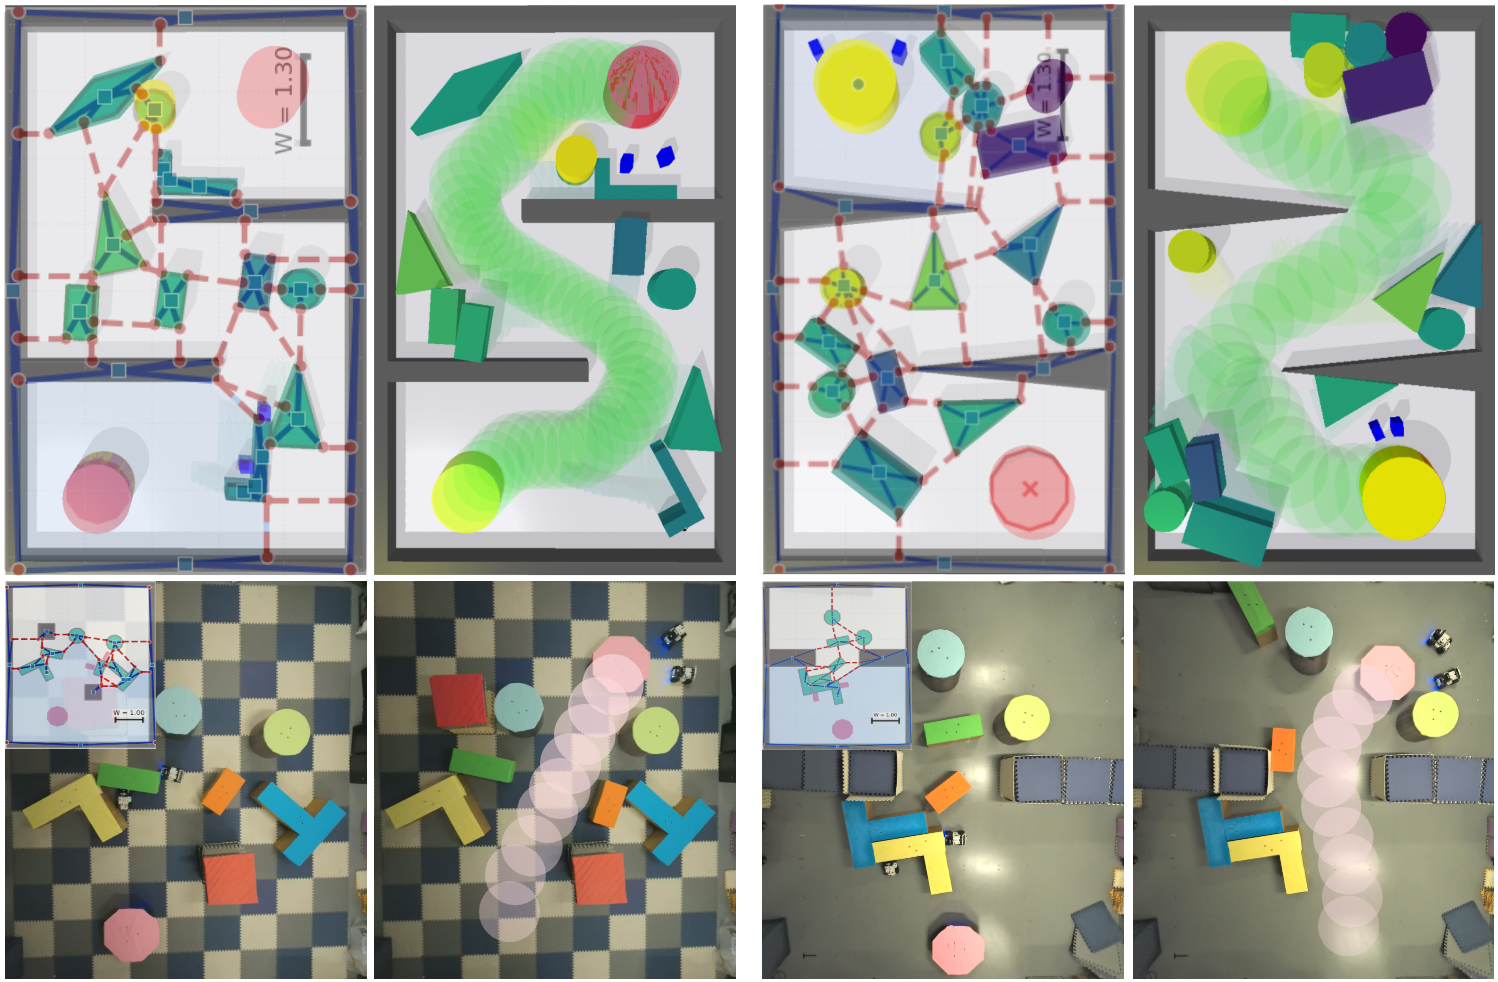
\includegraphics[width=0.9\linewidth]{figures/cover.png}% or {presearch.pdf}
  \vspace{-0.1in}
  \caption{
    Collaborative path clearing in simulation (\textbf{Top})
    and hardware (\textbf{Bottom}). Two robots push movable obstacles to
    create a $W$--clear path for a large vehicle from start to goal.
  }
  \vspace{-6mm}
  \label{fig:snapshots}
\end{figure}

%==============================================

\subsection{Related Work}\label{subsec:intro-related}

\looseness=-1
NAMO extends motion planning to cluttered environments by planning obstacle
displacements through pushing, pulling, or
rotating~\cite{stilman2005navigation,stilman2007manipulation}. Later work considers heuristic search, learning-based local planning, physics-based rollouts, and collaborative pushing~\cite{stilman2007manipulation,yao2024local,ren2025search,weeda2025pushing,tang2026pushingbots}.



%==============================================
\begin{figure*}[t!]
  \centering
  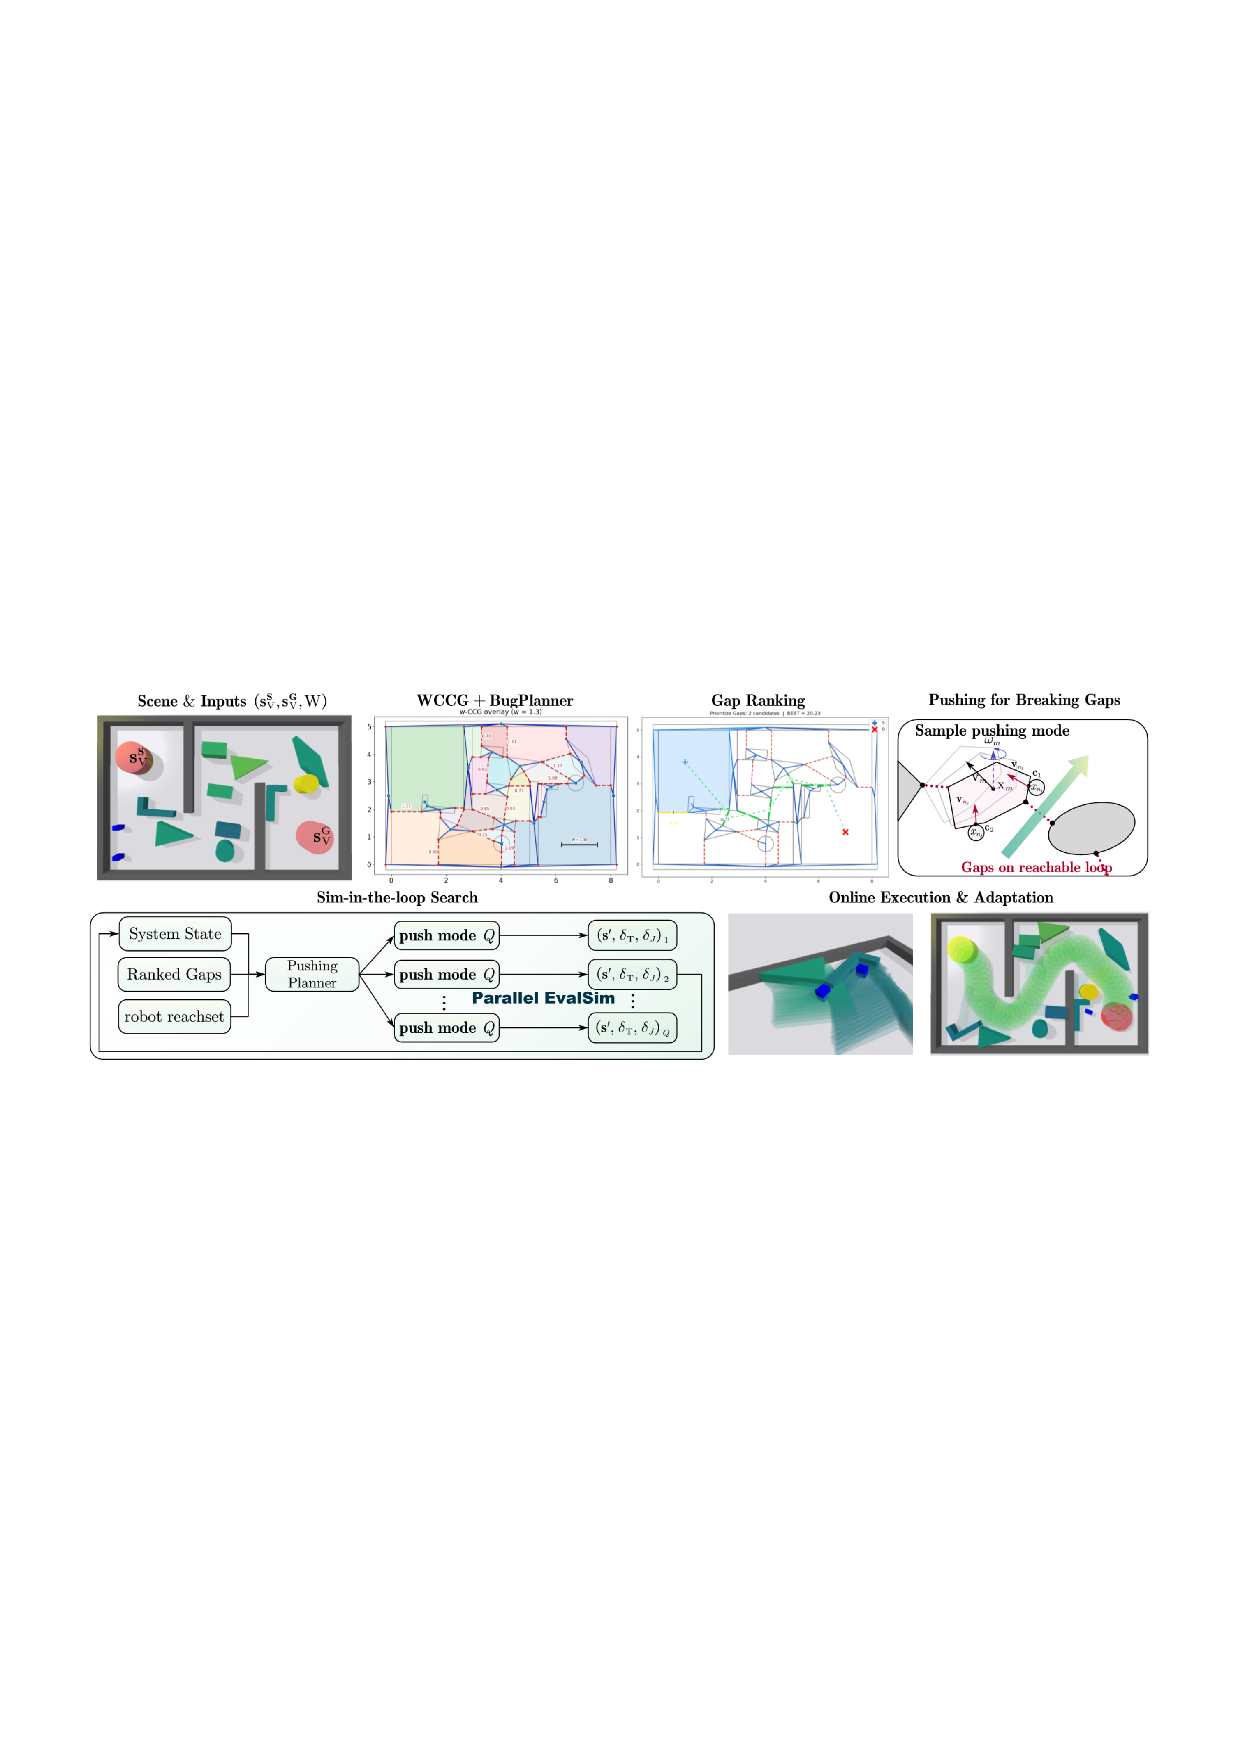
\includegraphics[width=0.84\linewidth]{figures/overall.pdf}
  \vspace{-0.1in}
\caption{Overview of the proposed framework.
\textbf{Top:} Scene inputs, WCCG construction, gap ranking, and sampling of pushing
modes for breaking frontier gaps;
\textbf{Bottom-left:} Sim-in-the-loop hybrid search with parallel validation in simulation;
\textbf{Bottom-right:} Online execution and adaptation during path clearing.}
  \label{fig:overall}
  \vspace{-5mm}
\end{figure*}
%==============================================


Collaborative pushing has been widely studied in multi-robot manipulation:
foundational work on the mechanics of pushing and limit surfaces~\cite{goyal1989limit,lynch1992manipulation}, cooperative transport with robot swarms~\cite{chen2015occlusion}, multi-robot box pushing with reinforcement learning~\cite{wang2006multi}, collaborative pushing of polytopic objects in cluttered scenes~\cite{tang2026pushingbots}, and learning-based loco-manipulation~\cite{feng2025learning}. These studies focus on a prescribed object rather than multi-object corridor clearing.

Physics-informed planning incorporates dynamics models, contact reasoning, or
simulation feedback into motion generation: learned dynamics for humanoid
contact planning~\cite{lin2019efficient}, multi-contact force control~\cite{rouxel2024multi}, demonstration-guided optimal control over contact modes~\cite{xue2023demonstration}, physics simulation interleaved with multi-agent pathfinding~\cite{saxena2023planning,ren2025object}, and learned physical priors~\cite{ni2023progressive,liu2025physics}. \change{These methods consider a prescribed target or few objects, whereas corridor clearing requires rearranging many obstacles to admit a larger vehicle.}


%==============================
\subsection{Our Method}\label{subsec:intro-our}

As shown in Fig.~\ref{fig:overall}, this work introduces \textbf{PushAround},
a physics-informed framework for collaborative multi-robot pushing that
constructs traversable corridors for large vehicles in cluttered environments.
Its central novelty is a hybrid search that jointly determines which obstacles
to displace and how to push them, coupling the high-level clearing sequence
with low-level pushing modes specifying contact points, directions and forces.
The framework integrates a W--clearance connectivity graph (WCCG) that certifies
vehicle passage under width constraints, frontier-gap ranking by estimated
effort, and pushing-mode generation under geometric and actuation constraints.
Guided by the selected gap, the search proposes direct pushes or recursively
clears blocking obstacles, and expands the plan through physics-validated
transitions that account for robot dimensions, object mass, contact geometry
and coupled pushing dynamics. Execution feedback updates connectivity and
triggers replanning when needed.
% \change{We further examine its robustness to physical-model uncertainty relevant to real-world deployment.}



The contributions are twofold: {(I)} it introduces a unified framework that
couples collaborative pushing with physics-informed verification, 
producing executable plans for path clearing in cluttered environments; 
and {(II)} \change{ 
it demonstrates empirical gains in feasibility, efficiency and scalability over evaluated NAMO and
collaborative-clearing baselines, with robustness to execution-side physics
mismatch.
}

%%========================================
\section{Problem Description}\label{sec:problem}
%==============================
\subsection{Workspace and Robots}\label{subsec:ws}
The workspace is a bounded planar region $\mathcal{W}\subset\mathbb{R}^2$
containing immovable structures~$\mathcal{O}\subset\mathcal{W}$ and $M\geq0$
movable rigid polygons
$\boldsymbol{\Omega}\triangleq\{\Omega_1,\cdots,\Omega_M\}\subset\mathcal{W}$.
Each movable obstacle~$\Omega_m$ has mass~$\mathsf{M}_m$,
inertia~$\mathsf{I}_m$, frictional parameters and state
$\mathbf{s}_m(t)\triangleq(\mathbf{x}_m(t),\psi_m(t))$, with
$\mathbf{x}_m(t)\in\mathbb{R}^2$ the centroid position and
$\psi_m(t)\in\mathbb{R}$ the orientation; $\Omega_m(t)$ denotes the region it
occupies at time~$t$. A team of~$N$ robots,
$\mathcal{R}\triangleq\{R_1,\cdots,R_N\}$, operates as a cooperative unit. Each
robot~$R_i$ is a rigid body with state
$\mathbf{s}_{R_i}(t)\triangleq(\mathbf{x}_{R_i}(t),\psi_{R_i}(t))$ and
footprint~$R_i(t)$. The instantaneous free space is given by:
\begin{equation}\label{eq:freespace}
\widehat{\mathcal{W}}(t)\triangleq\mathcal{W}\setminus\Big(
\mathcal{O}\cup\{\Omega_m(t)\}_{m=1}^{M}\cup\{R_i(t)\}_{i=1}^{N}
\Big),
\end{equation}
where~$\widehat{\mathcal{W}}(t)$ excludes regions occupied by immovable
obstacles, movable obstacles, and robots.

%==============================
\subsection{External Vehicle and Clearance Goal}\label{subsec:vehicle}
An external vehicle~$\texttt{V}$ whose footprint is enclosed by a disk of
radius~$W/2>0$ must navigate within the workspace from a start position
$\mathbf{x}_\texttt{V}^{\texttt{S}}\in\mathcal{W}$ to a goal position
$\mathbf{x}_\texttt{V}^{\texttt{G}}\in\mathcal{W}$. Since movable obstacles may
obstruct the way, the clearance goal is to rearrange them so that the workspace
contains a passage from~$\mathbf{x}_\texttt{V}^{\texttt{S}}$ to
$\mathbf{x}_\texttt{V}^{\texttt{G}}$ that can accommodate this enclosing disk,
i.e., a passage of width at least~$W$. At time~$t$, this is expressed by the
admissible reference-center space
$\mathcal{F}_W(t)\triangleq
\{p\in\widehat{\mathcal{W}}(t)\mid
\mathbb{B}_{W/2}(p)\subset\widehat{\mathcal{W}}(t)\}$, where
$\mathbb{B}_{W/2}(p)$ is the disk of radius~$W/2$ centered at~$p$. The
$W$-clearance condition is then given by:
\begin{equation}\label{eq:wclear}
\exists\,\mathcal{P}^W_\texttt{V}\subset\mathcal{F}_W(t):\
\mathbf{x}_\texttt{V}^{\texttt{S}}\leadsto\mathbf{x}_\texttt{V}^{\texttt{G}},
\end{equation}
which certifies a collision-free centerline path for any vehicle footprint
contained in the enclosing disk.
% Since movable obstacles may obstruct the way,
% a direct passage is not always feasible.
% At time~$t$, the admissible center positions of~$\texttt{V}$ are
% \begin{equation}
% \mathcal{F}_W(t)\triangleq
% \{p\in\widehat{\mathcal{W}}(t)\mid \mathbb{B}_{W/2}(p)\subset\widehat{\mathcal{W}}(t)\}.
% \end{equation}
% where $\mathbb{B}_{W/2}$ is a disk of radius~$W/2$.
% The clearance goal is satisfied if there exists a continuous centerline path
% inside~$\mathcal{F}_W(t)$:
% \begin{equation}\label{eq}
% \exists\,\mathcal{P}^W_\texttt{V}\subset\mathcal{F}_W(t):
% \mathbf{x}_\texttt{V}^{\texttt{S}}\leadsto\mathbf{x}_\texttt{V}^{\texttt{G}}.
% \end{equation}
% this therefore certifies a passage with width at
% least~$W$.


%==============================


\subsection{Collaborative Pushing Modes}\label{ss:interaction_mode}
To enlarge blocked gaps, the robots may actively
reconfigure~$\boldsymbol{\Omega}$ by pushing movable obstacles. For obstacle
$\Omega_m\in\boldsymbol{\Omega}$, a pushing mode is denoted by
$\boldsymbol{\xi}_m\triangleq(\mathbf{c}_m,\mathbf{u}_m)$, where
$\mathbf{c}_m=(c_1,\cdots,c_N)$ is an ordered tuple of contact points on
$\partial\Omega_m$, and the ordering specifies the robot-to-contact assignment.
The vector~$\mathbf{u}_m\in\mathbb{R}^{2N}$ stacks the corresponding planar
contact forces, expressed in the body frame of~$\Omega_m$; \change{an inactive
robot carries a null contact $c_i=\varnothing$ with zero force.}
For a contact tuple~$\mathbf{c}_m$, the set of admissible forces
${U}_m(\mathbf{c}_m)\subset\mathbb{R}^{2N}$ collects contact forces
satisfying the robot pushing limits, robot--object friction, and unilateral
contact constraints. The body wrench induced by a mode is defined as:
\begin{equation}
\mathbf{q}_m(\boldsymbol{\xi}_m)
\triangleq
G_m(\mathbf{c}_m)\mathbf{u}_m,
\label{eq:contact_wrench_map}
\end{equation}
where~$G_m(\mathbf{c}_m)\in\mathbb{R}^{3\times 2N}$ is the contact-to-wrench mapping;
and $\mathbf{q}_m(\boldsymbol{\xi}_m)\in\mathbb{R}^3$.
The admissible mode set is state dependent as denoted by~$\Xi_m(\mathbf{s})$.
It contains modes whose contacts are reachable from the
current robot configurations, pre-contact configurations are feasible in
the current clutter, and forces satisfy
$\mathbf{u}_m\in{U}_m(\mathbf{c}_m)$. Hence, applying a feasible
mode~$\boldsymbol{\xi}_m\in\Xi_m(\mathbf{s}(t))$ yields the physical
transition:
\begin{equation}\label{eq:transition}
  \mathbf{s}(t^+)\triangleq
  \Phi\big(\mathbf{s}(t),\,m,\,\boldsymbol{\xi}_m\big),
\end{equation}
where~$\mathbf{s}(t)$ stacks all robot and obstacle states.
\change{
The force vector~$\mathbf{u}_m$ serves as a feasibility variable to certify
wrench generation under the modeled contact and actuation constraints rather
than a directly commanded control input.
}


%==============================
\subsection{Problem Statement}\label{subsec:objective}

The goal is to compute a \emph{hybrid schedule} that reconfigures movable
obstacles to admit a $W$-feasible path for the external vehicle.
The schedule is defined as:
\begin{equation}\label{eq:schedule}
    \pi\triangleq
    \left\{
    \left(
    \Omega_{m_k},
    \mathbf{v}_k,
    \boldsymbol{\xi}_k
    \right)
    \right\}_{k=1}^{K},
\end{equation}
where~$\Omega_{m_k}\in\boldsymbol{\Omega}$ is the manipulated obstacle,
$\mathbf{v}_k$ its pushing direction, $\boldsymbol{\xi}_k\in\Xi_{m_k}$ its
pushing mode. The node cost is:
\begin{equation}\label{eq:problem}
    \mathcal{J}_{\mathrm{clr}}(\pi)
    \triangleq
    T+
    \alpha
    \sum_{k=1}^{K}
    J\left(
    m_k,\boldsymbol{\xi}_k,\mathbf{s}(t_k)
    \right),
\end{equation}
\change{where~$T\triangleq\sum_{k=1}^{K}\Delta t_k$ denotes 
the robotic clearance duration excluding vehicle traversal,  
with $\Delta t_k>0$ the duration that the evaluation in~(13) returns for the $k$-th push,
 and~$J(\cdot)$ is the simulation-estimated manipulation cost. 
 Vehicle traversal enters only through the terminal $W$-clearance condition~\eqref{eq:wclear}. 
 The constraints~\eqref{eq:freespace}--\eqref{eq:transition} 
 enforce valid pushing transitions. 
 Equation~\eqref{eq:problem} defines the realized clearance cost; PIHS samples finitely and does not guarantee optimality.}

% ==============================
\begin{remark}\label{remark:uniqueness}
  \change{The objective couples obstacle selection, pushing-mode generation and switching into one hybrid planning problem, yielding a combinatorial-continuous search space richer than classical NAMO formulations with hand-crafted contact modes~\cite{goyal1989limit,chen2015occlusion,wang2006multi}.}
  \hfill~$\blacksquare$
\end{remark}
% ==============================

%%========================================
% %% ========================================
\section{Proposed Solution}\label{sec:solution}

As shown in Figs.~\ref{fig:overall} and~\ref{fig:pihs_overview}, PushAround first
uses the W-Clearance
Connectivity Graph in Sec.~\ref{subsec:wccg} and gap ranking in
Sec.~\ref{subsec:gap} to identify and prioritize blocking gaps. It then
generates and evaluates physically feasible collaborative pushing modes in
Sec.~\ref{subsec:push}. These components are integrated into the
simulation-in-the-loop hybrid search of Sec.~\ref{subsec:simloop} and the online
execution procedure of Sec.~\ref{subsec:overall}.





% %% ========================================
\input{contents/wccg.tex}
% %% ========================================
\input{contents/gap.tex}
% %% ========================================
\input{contents/push.tex}
% %% ========================================
\input{contents/simloop.tex}
% %%========================================
\input{contents/overall.tex}
% %%========================================

%%========================================
% ============================================================
\section{Experiments}
\label{sec:experiments}
We evaluate PIHS in simulation and hardware (see accompanying video).
The algorithms are implemented in \texttt{Python3} and \texttt{PyBullet}~\cite{coumans2019}
on a machine with an Intel i9-14900KF and an RTX 4080.
\subsection{Numerical Simulations}
\label{subsec:sim}
% ========================================
\begin{table}[t]

\centering

\caption{\change{WCCG connectivity validation and mean runtime.}}

\label{tab:wccg-validation}

\vspace{-2.0mm}

\footnotesize

\setlength{\tabcolsep}{3.8pt}
\setlength{\belowrulesep}{0.30ex}
\renewcommand{\arraystretch}{0.86}

\change{
\begin{tabular}{
 @{}
 l
 cc
 @{\hspace{8pt}}
 ccc
 @{}
}

\toprule

&
\multicolumn{2}{c}{Validation}
&
\multicolumn{3}{c}{Runtime (ms)}
\\[-0.6ex]

\cmidrule(lr){2-3}
\cmidrule(lr){4-6}

Type
& CC $=$ FR
& FP/FN$^\dagger$
& CC
& FR
& WCCG
\\

\midrule

Convex
& 100/100
& 0/0
& 1.23
& 282.9
& \textbf{0.86}
\\

Non-convex
& 98/100
& 0/0
& 1.51
& 204.1
& \textbf{1.30}
\\

Mixed
& 98/100
& 0/0
& 1.33
& 242.4
& \textbf{1.05}
\\

\midrule

Total
& 296/300
& \textbf{0/0}
& 1.36
& 243.1
& \textbf{1.07}
\\

\bottomrule

\end{tabular}
}

\vspace{0.5mm}

{\scriptsize
\change{
$^\dagger$WCCG errors relative to the continuous configuration-space reference (CC).
All runtimes use the same 300-scene harness with the compiled WCCG backend.
}
}

\vspace{-5.5mm}

\end{table}

\subsubsection{Setup and Configuration}\label{subsec:sim-setup}

The simulation runs at a step size of $\Delta t=1/240$\,s with a control period
of $1/40$\,s; robots are disk or box pushers consistent with the $W$-clearance
definition, and movable obstacles have masses $[5,15]$\,kg in Scenarios~1--2, $[20,30]$\,kg in the generalization studies. A trial
succeeds when the external vehicle reaches its goal through a $W$-clear path. The
nominal scenario is an $8\times5$\,m workspace with bottleneck-forming bar
obstacles, where two robots clear $10$--$15$ movable obstacles under
minimum-separation constraints. Unless stated otherwise, comparisons and
ablations use Scenario~1 ($10$ movable obstacles, $40$ trials), and Scenario~2
($14$ obstacles) provides an additional cluttered case
(Fig.~\ref{fig:main_result}). \change{All methods share the robot footprints,
obstacle configurations, collision and reachability checks, and execution
simulator, with the same $800$\,s planning cap, $20{,}000$-step ($500$\,s) execution cap and $8$ workers. Unless stated otherwise, times average over successful trials, failures counting only in the success rate; the scalability curves instead cap failures.}



% ========================================
\begin{table}[t]
 \centering
 \begin{threeparttable}
 \caption{Performance comparison and ablations on Scenario~1 over $40$ randomized trials.\tnote{a}}
 \label{tab:main_ablation}
 \setlength{\tabcolsep}{2.7pt}
 \renewcommand{\arraystretch}{0.92}
 \begin{tabular}{lccccc}
 \toprule
 Method / Variant & Succ.(\%) & PT (s) & ET (s) & \#Sims & \#Pushes \\
 \midrule
 DFS-WCCG & 25.0 & $>$100.0 & 51.2 & $>$500 & 8.0 \\
 SL-Push (offline) & 62.5 & 0.06 & 44.1 & 0.0 & 7.3 \\
 SL-Push (sim) & 75.0 & 18.2 & 64.6 & 20.0 & 10.2 \\
 Rec-NAMO & 37.5 & 13.3 & 42.4 & 0.0 & 7.8 \\
 \textbf{PushAround (ours)}
 & \textbf{97.5} & \textbf{10.3} & \textbf{28.6}
 & \textbf{121.5} & \textbf{6.0} \\
 \midrule
 w/o gap-lookahead & 82.5 & 16.9 & 35.2 & 178.3 & 7.2 \\
 w/o mode-cache & 92.5 & 17.1 & 33.4 & 164.6 & 6.5 \\
 w/o quick-pass & 90.0 & 23.6 & 41.9 & 208.2 & 6.1 \\
 w/o reinsertion & 85.0 & 12.8 & 31.1 & 151.7 & 7.8 \\
 \bottomrule
 \end{tabular}
 \begin{tablenotes}\scriptsize
 \item[a] Times are averaged over successful trials; failures count in the
 success rate only. For DFS-WCCG, $PT$ and
 \#Sims are not comparable and are given as lower bounds ($>$).
 \end{tablenotes}
 \end{threeparttable}
 \vspace{-4.0mm}
\end{table}

% ========================================
% ========================================
\begin{figure}[t!]
 \centering
 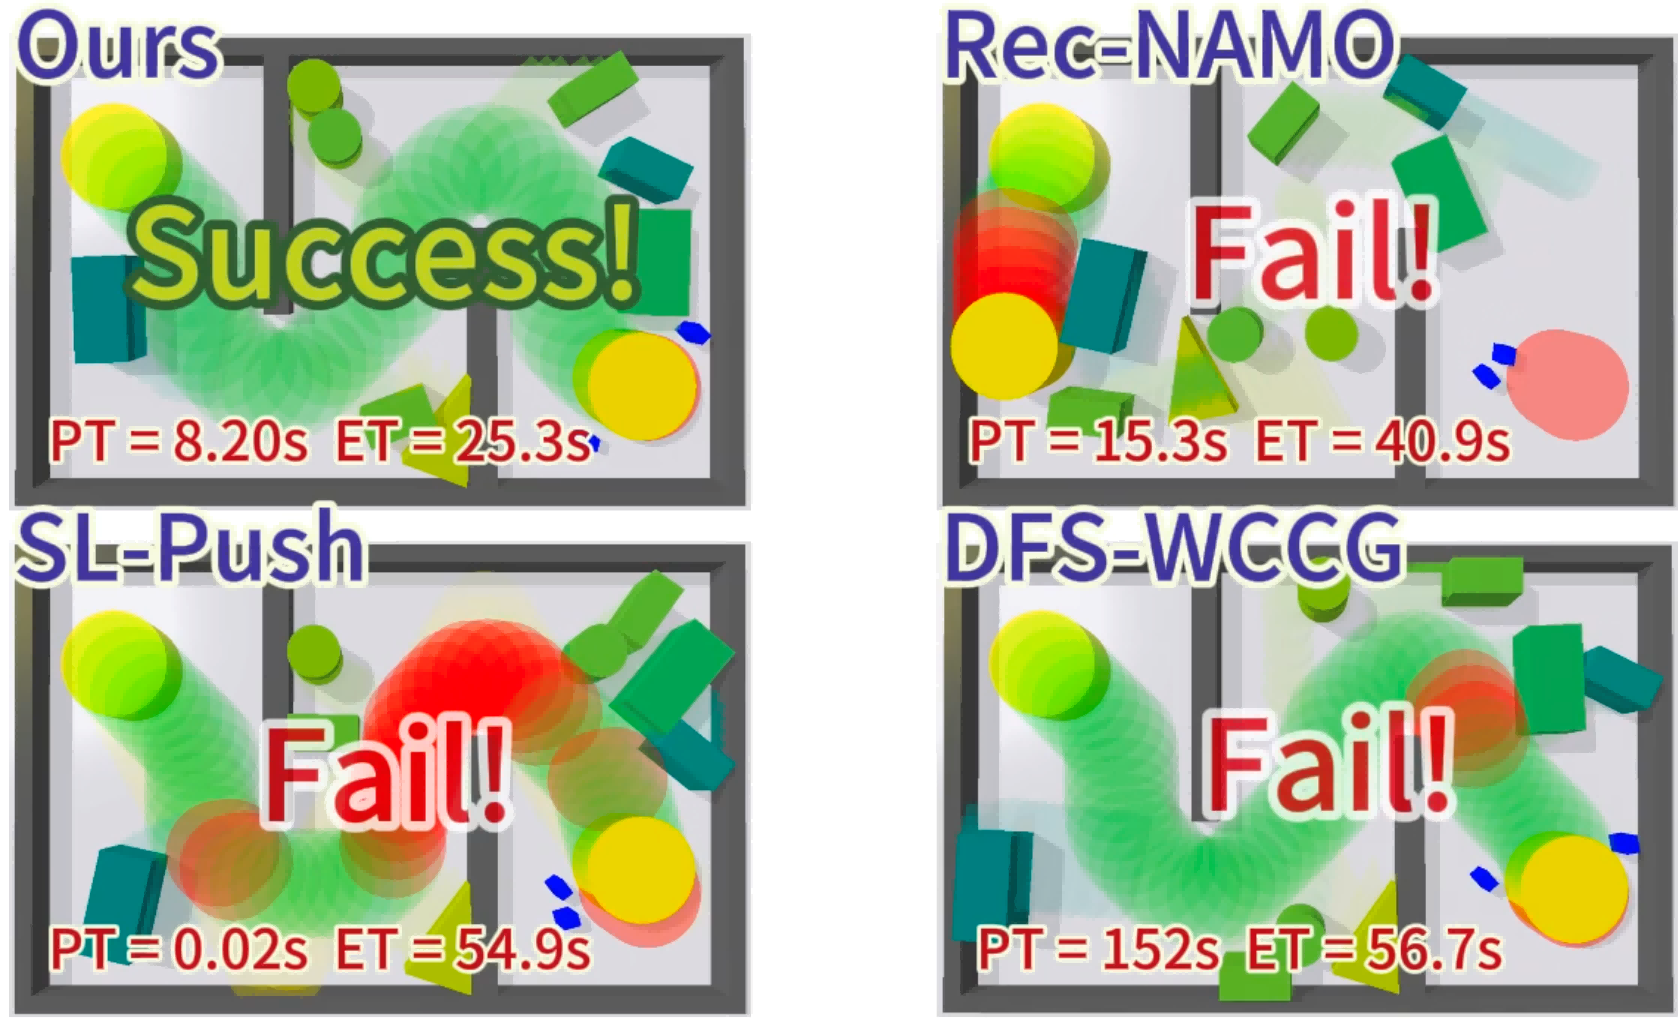
\includegraphics[width=0.7\columnwidth]{figures/compare.png}
 \vspace{-3.0mm}
 \caption{Failure cases by baselines Rec-NAMO, SL-Push and DFS-WCCG.}
 \label{fig:baseline}
 \vspace{-6.0mm}
\end{figure}

% ========================================
%==============================
\subsubsection{Results}
\change{
Across the $40$ Scenario~1 trials, PushAround achieves a $97.5\%$ success rate,
with mean planning and execution times of $10.3$\,s and $28.6$\,s, respectively,
and $6.0$ pushes per successful trial, as shown in Table~\ref{tab:main_ablation}.
Fig.~\ref{fig:main_result} shows representative runs in both scenarios.
In Scenario~1 with $10$ movable obstacles and two robots, PushAround generates
a $6$-push plan in $7.4$\,s and completes execution in $42.3$\,s. In
Scenario~2 with $14$ obstacles, it generates a $9$-push plan in $11.2$\,s,
with $61.3$\,s of execution.
Planning effort is dominated by simulation-based validation: a successful
trial uses $121.5$ simulations on average for $6.0$ executed pushes. The
ablations indicate that mode caching, quick-pass, gap lookahead, and reinsertion
mainly affect this validation load rather than plan length. Execution takes
longer because each selected push is physically carried out and observed,
whereas inter-push repositioning is handled by geometric reachability checks.
}

\change{
\subsubsection{WCCG Connectivity Validation}
\label{subsec:wccg-validation}

WCCG is compared against two references on $300$ random scenes (convex,
non-convex and mixed; Table~\ref{tab:wccg-validation}). The continuous reference (CC) resolves collisions geometrically after inflating boundaries by~$W/2$, with no grid discretization~\cite{lozano1983spatial}; the fine-raster reference (FR) discretizes the workspace on a $0.01$\,m occupancy grid. CC and FR disagree in $4$ of $300$ cases, all near narrow contacts and rasterization-related, whereas WCCG matches CC on all $300$ scenes without false positives or negatives. A query costs $1.07$\,ms ($0.67$\,ms query, $0.40$\,ms construction)
against $1.36$\,ms (CC) and $243$\,ms (FR). It also supplies the gap graph for PIHS. Rebuilt after every simulated or executed push, it is negligible next to the physics rollouts.
}




\subsubsection{Comparisons}\label{subsec:comparisons}
Four baseline variants run on Scenario~1 over $40$ randomized trials under the same $W$-clearance criterion, distribution and simulator:
\textbf{DFS-WCCG} (WCCG-guided search with fixed pushes), \textbf{SL-Push}
(offline and simulation-validated variants), and \textbf{Rec-NAMO} (recursive
NAMO)~\cite{stilman2007manipulation,yao2024local,saxena2023planning,ren2025search}.
Table~\ref{tab:main_ablation} shows that PushAround reaches the highest success
rate, $97.5\%$, at the lowest combined planning-and-execution time among
successful trials ($38.9$\,s).
DFS-WCCG exhibits rapid branching growth, offline SL-Push produces displacements that fail in execution, and Rec-NAMO often fails to connect the $W$-clear corridor in clutter (Fig.~\ref{fig:baseline}).


%==============================
\begin{table}[t]

\caption{\change{Scalability and robustness.}}
\label{tab:generalization}
\vspace{-2.0mm}
\centering
\footnotesize

\renewcommand{\arraystretch}{0.95}
\setlength{\tabcolsep}{3.5pt}

\change{
\begin{tabular}{
 @{}
 l
 c
 c
 r@{\;}c@{\;}l
 @{\hspace{10pt}}
 r@{\;}c@{\;}l
 @{}
}
\hline

Case
& Trials
& Succ.(\%)
& \multicolumn{3}{c@{\hspace{10pt}}}{$PT$ (s)}
& \multicolumn{3}{c}{$ET$ (s)}
\\

\hline

\multicolumn{9}{l}{
 \emph{Obstacle density} (PushAround, $N=2$, nominal)
}
\\

$M=15$
& 10 & 100
& 2.5 & $\pm$ & 0.9
& 37.1 & $\pm$ & 21.0
\\

$M=30$
& 10 & 100
& 11.7 & $\pm$ & 3.7
& 100.9 & $\pm$ & 34.7
\\

$M=45$
& 10 & 100
& 53.4 & $\pm$ & 24.5
& 272.7 & $\pm$ & 97.4
\\

\hline

\multicolumn{9}{l}{
 \emph{Robot-team size} ($M=30$, nominal; 10 trials per cell)
}
\\

PushAround, $N=3$
& 10 & 100
& 30.0 & $\pm$ & 12.7
& 97.3 & $\pm$ & 42.1
\\

PushAround, $N=4$
& 10 & 100
& 29.2 & $\pm$ & 8.9
& 110.1 & $\pm$ & 33.1
\\

SL-Push (sim), $N=3$
& 10 & 80
& 30.0 & $\pm$ & 46.3
& 193.3 & $\pm$ & 111.3
\\

SL-Push (sim), $N=4$
& 10 & 80
& 23.4 & $\pm$ & 18.2
& 171.7 & $\pm$ & 61.2
\\

DFS-WCCG, $N=3$
& 10 & 100
& 142.6 & $\pm$ & 183.1
& 178.1 & $\pm$ & 72.1
\\

DFS-WCCG, $N=4$
& 10 & 90
& 101.9 & $\pm$ & 103.9
& 175.9 & $\pm$ & 113.6
\\

\hline

\multicolumn{9}{l}{
 \emph{Physics mismatch} ($M=30$, $N=2$)
}
\\

Nominal
& 10 & 100
& 16.8 & $\pm$ & 3.4
& 104.7 & $\pm$ & 37.4
\\

Mass $\times 0.6$--$1.4$
& 40 & 100
& 16.8 & $\pm$ & 5.4
& 105.9 & $\pm$ & 44.6
\\

Lateral fric. $\times 0.6$--$1.4$
& 40 & 97.5
& 16.5 & $\pm$ & 5.7
& 114.0 & $\pm$ & 48.5
\\

Spin fric. $\times 0.6$--$1.4$
& 40 & 97.5
& 15.2 & $\pm$ & 3.6
& 100.1 & $\pm$ & 35.7
\\

Force limit $\times 0.6$--$1.4$
& 40 & 95.0
& 18.9 & $\pm$ & 10.9
& 115.9 & $\pm$ & 58.5
\\

All perturbed
& 160 & 97.5
& 16.9 & $\pm$ & 7.0
& 108.9 & $\pm$ & 47.4
\\

\hline

\end{tabular}
}

\vspace{0.5mm}

\begin{flushleft}
\footnotesize
\change{
Each perturbed row scales one parameter; the others stay nominal. Times and budget
are as in Table~\ref{tab:main_ablation}.
}
\end{flushleft}

\vspace{-6.0mm}

\end{table}

%==============================

%==============================
\subsubsection{Ablation Studies}
Four internal ablations are conducted: \textbf{w/o gap-lookahead} (gaps ranked
without downstream costs), \textbf{w/o mode-cache} (no warm start from validated
modes), \textbf{w/o quick-pass} (all candidates evaluated by rollout), and
\textbf{w/o reinsertion} (failed nodes not reconsidered).
Table~\ref{tab:main_ablation} shows that gap-lookahead and reinsertion mainly
improve robustness (success drops by more than $10\%$ when either is removed),
whereas quick-pass also lowers success to $90.0\%$ and mode-cache mainly changes
the simulation count.


\change{

\subsubsection{Scalability and Robustness Analysis}
\label{subsec:generalization}

Generalization studies use an $8\times8$\,m workspace
(Table~\ref{tab:generalization}, Figs.~\ref{fig:scalability_scenes}--\ref{fig:density_scaling}).
\minorchange{Density runs query a precomputed mode table (preparation excluded from $PT$);
mismatch and team-size runs optimize modes greedily. At $M{=}30$, $N{=}2$,
nominal $PT$ is $11.7$, $16.8$ and $23.9$\,s, respectively; the team-size
study uses a different scene realization of the same seeds.}
\textbf{(I) Obstacle density:} with two robots, $10$ trials per density,
PushAround keeps $100\%$ success at all tested densities ($M{=}15$ to $45$), planning in $2.5$--$53.4$\,s; at $M{=}45$ none of the evaluated baselines solves any trial
and the no-recursion ablation solves $7/10$.
\textbf{(II) Robot-team size:} at $M{=}30$, PushAround solves all ten trials at
$N{=}2$, $3$, and $4$ using the same mode-generation
procedure with a full-team-first fallback that may leave one robot temporarily inactive.
Across the clutter sweep, branching stays near six while expansions rise
from $3.5$ to $24.5$. A solved trial needs a median of $10$ expansions and
$48$ visited snapshots and about $60$ simulations at $165$\,ms each,
against $22$\,ms per generated mode. Across $N{=}2$--$4$, search effort remains similar
($10$ expansions, $60$--$63$ simulations), while aggregate mode-generation
time rises from $15.8$ to $46.4$\,s.
\textbf{(III) Physics mismatch:} the planner keeps the nominal model and only
the execution simulator is perturbed, one parameter at a time.
PushAround solves $156/160$ perturbed trials ($97.5\%$); under $\pm40\%$
perturbations SL-Push (sim) solves $13/40$ and DFS-WCCG $23/40$.
Averaging successful-trial $PT$ over conditions with successes gives $31.5$
and $229.1$\,s, versus $18.4$\,s for PushAround.
\minorchange{These paired, single-parameter trials reuse ten base seeds (five for
baselines), whose nominal success is $3/5$ versus $10/10$ for PushAround.
Comparisons reflect end-to-end performance rather than normalized
degradation; joint parameter errors are untested.}

}



% ========================================
\begin{figure}[t!]
 \centering
 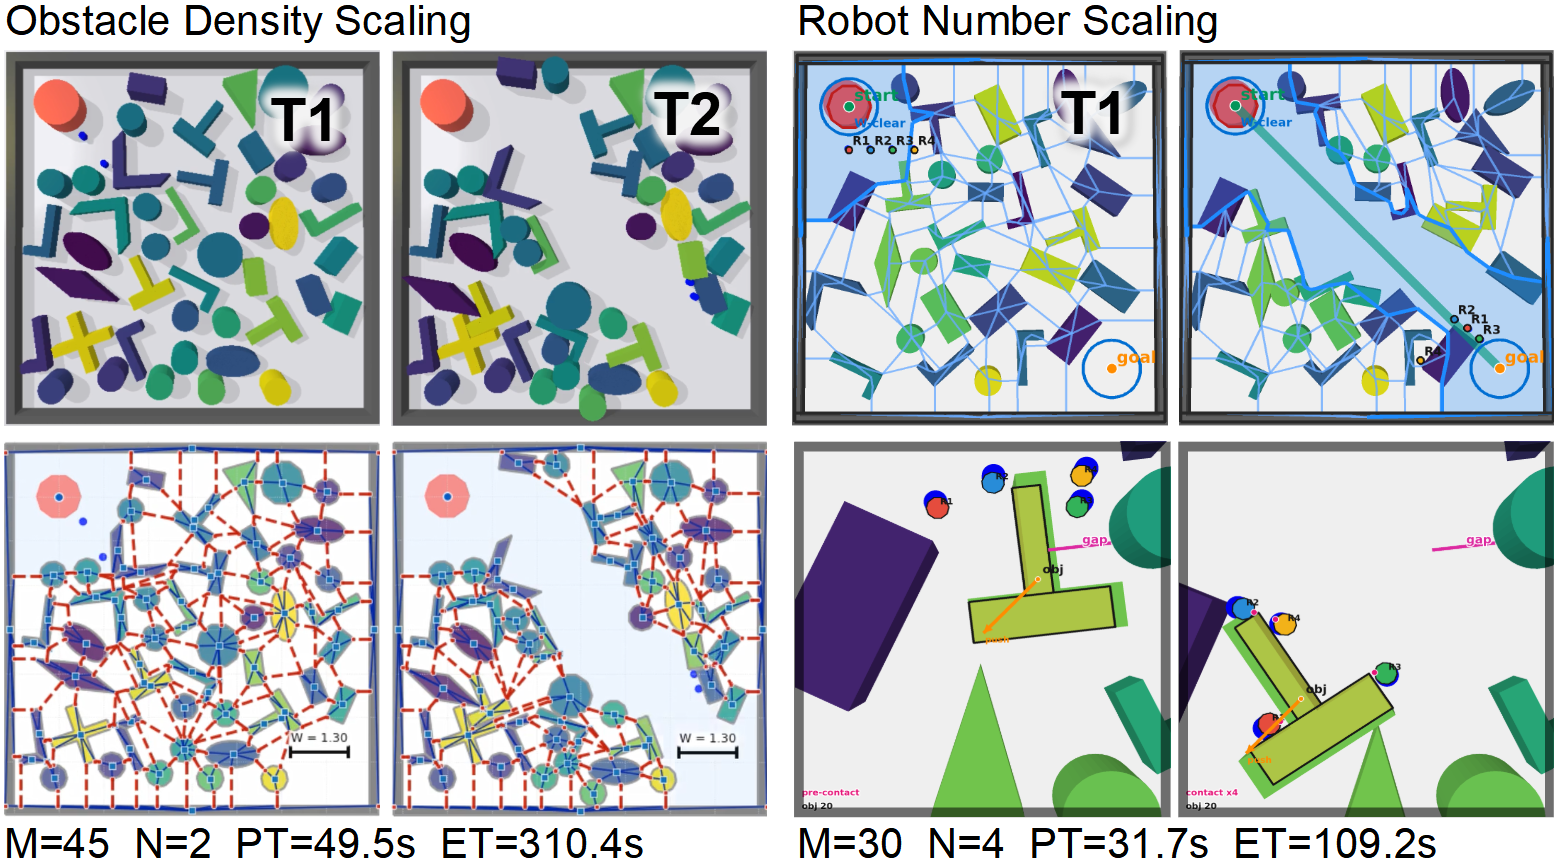
\includegraphics[width=0.9\columnwidth]{figures/obs_rob_scale.png}
 \vspace{-2mm}
 \caption{\change{
 Scalability of the clearing process. \textbf{Left:} density scaling ($M{=}45$, two robots): snapshots during clearing (\textbf{top}) and WCCG overlays with the start face in blue (\textbf{bottom}). \textbf{Right:} team scaling ($M{=}30$, four robots): initial and final states (\textbf{top}) and one push before contact and during execution (\textbf{bottom}).}}
 \label{fig:scalability_scenes}
 \vspace{-3mm}
\end{figure}

% ========================================
% ========================================
\begin{figure}[t!]
 \centering
 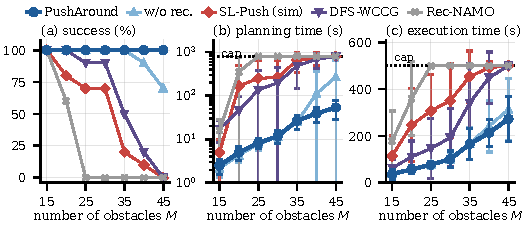
\includegraphics[width=0.95\columnwidth]{figures/density_comparison.pdf}
 \vspace{-2.0mm}
 \caption{\change{
 Obstacle-density scaling ($8\times 8$\,m, $10$ seeds per density). Times are
 budget-capped (planning $800$\,s, execution $20{,}000$ steps $=500$\,s; dotted).}}
 \label{fig:density_scaling}
 \vspace{-4.0mm}
\end{figure}

% ========================================
% ========================================
% ========================================
\begin{figure*}[!t]
 \centering
 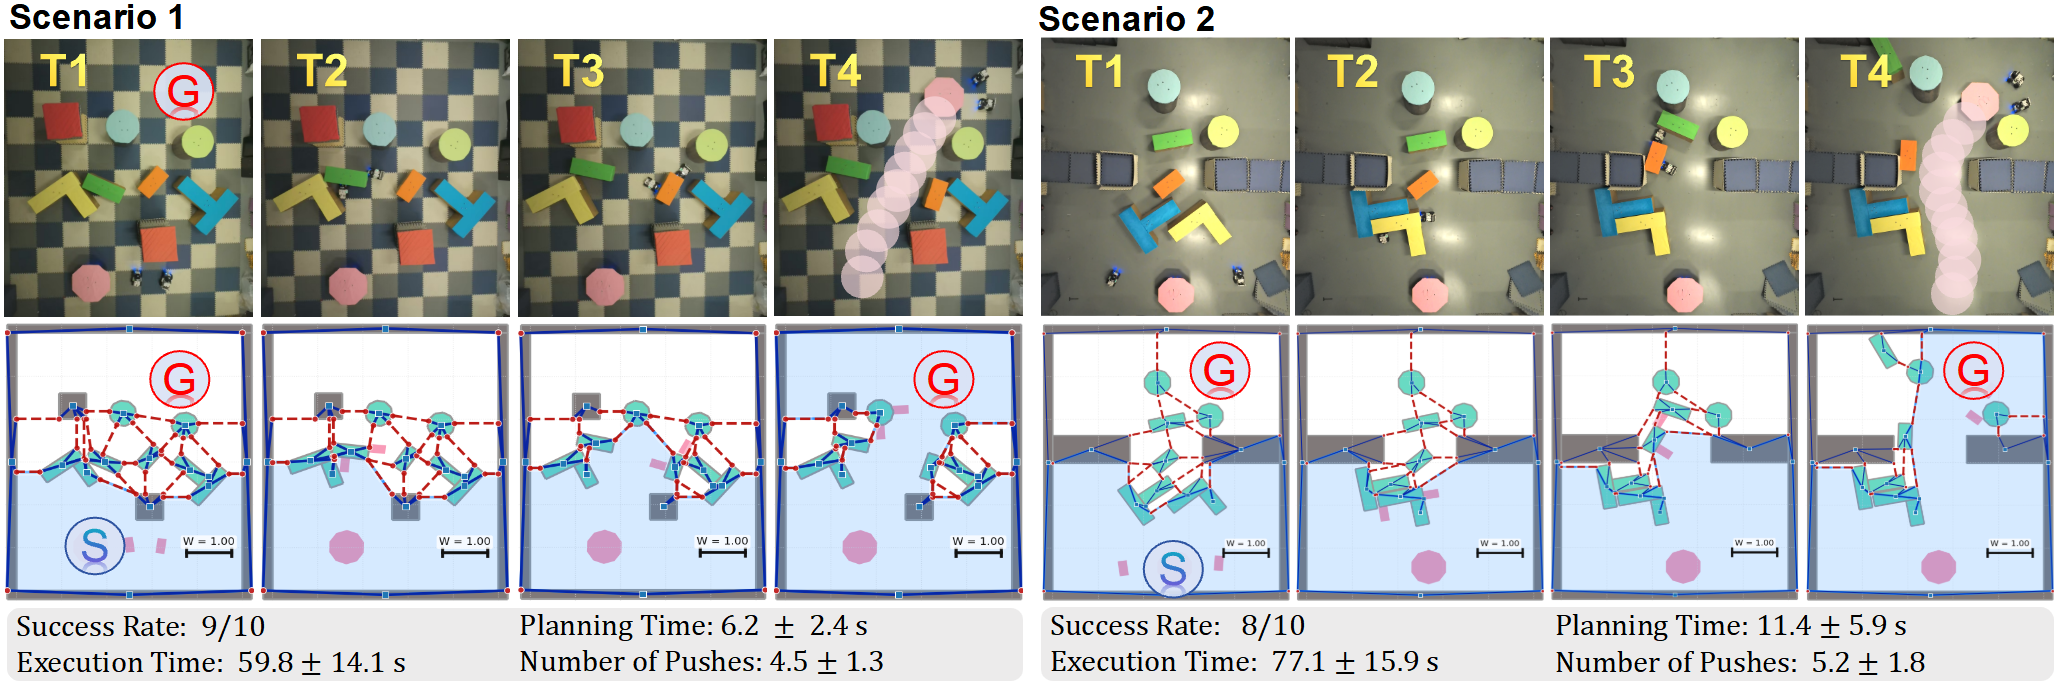
\includegraphics[width=0.95\linewidth]{figures/hardware.png}
 \vspace{-2.0mm}
 \caption{\change{Real-world pushing experiments with execution--planning alignment (over~$20$ runs, $2$ scenarios).
 \textbf{Top:} two robots pushing obstacles in a \(5{\times}6\,\mathrm{m}\)
 workspace. \textbf{Bottom:} WCCG overlays with the start face in blue.}}
 \vspace{-5.0mm}
 \label{fig:hardware}
\end{figure*}

\subsection{Hardware Experiments}\label{subsec:hardware}

\subsubsection{System Description}\label{subsec:exp-description}
Experiments use a $5\times6$\,m workspace of interlocking $0.6\times0.6$\,m foam mats (Fig.~\ref{fig:hardware}), $2$ UGVs and $6$ cardboard boxes; robots and movables carry motion-capture markers streamed to \texttt{PyBullet} in real time.
\change{The UGVs are velocity-controlled, and the optimized contact forces are used only for feasibility evaluation, not for motor control.
\minorchange{Motion-capture poses are compared with $\mathsf{EvalSim}$ predictions:
position or orientation errors above $0.3$\,m or $\pi/4$ trigger replanning,
as do the failures in Sec.~\ref{subsec:execute}.}}

\subsubsection{Results}\label{subsec:exp-results}
Two representative real-world runs are shown in Fig.~\ref{fig:hardware}.
In hardware Scenario~1, PIHS considers five candidate gaps and plans a four-task schedule in $6.5$\,s ($12$ node expansions, $49$ visited snapshots, search depth $6$); the robots then execute it, first rotating the yellow L-shaped object to open a gap near an
immovable obstacle and then separating the green and orange objects until a $W$--clear path is established at $t=52\,$s.
In hardware Scenario~2, PushAround succeeds in $8/10$ trials with an average of $5.2$
pushes and $11.4$\,s of planning; the first direct push on the blue L-shaped
object also moves the adjacent T-shaped block and opens the first gap.
\change{This neighboring-object motion is not a separately encoded action but
an emergent outcome of the coupled rigid-body rollout in $\mathsf{EvalSim}$,
whose snapshot updates the WCCG and execution continues.}
\change{\minorchange{Execution takes $77.1\pm15.9$\,s (mean $\pm$ standard deviation);}
online replanning compensates for deviations due to force limits,
drifting and wheel slippage.}

%%========================================
\section{Conclusion} \label{sec:conclusion}
\change{This work presents PushAround, a multi-robot framework that jointly plans
obstacle selection, contact points and pushing forces through a hybrid search,
and demonstrates hardware feasibility with state-feedback replanning. Future work
targets obstacle-state estimation without external sensing, uncertain masses and
limited robot visibility.}

%%========================================


%========================================
\bibliographystyle{IEEEtran}
\bibliography{contents/references}

\end{document}
"
\ifdefined\CLEANCOPY
  \renewcommand{\minorchange}[1]{#1}
\fi

%%%%%%%%%%%%%%%%%%%%%%%%%%%%%%%%%%%%%%%%%%%%%%%%%%%%%%%
%%%%


% Publication metadata for RA-L 26-3602.
% Author spellings, order, keywords and received date follow PaperCept.
% Revised and accepted dates confirmed by the author on October 20, 2026.
\newcommand{\RALReceivedDate}{June 24, 2026}
\newcommand{\RALRevisedDate}{September 16, 2026}
\newcommand{\RALAcceptedDate}{October 20, 2026}
% RA-L specifies the month/year of final submission in the preprint header.
\newcommand{\RALFinalMonthYear}{October, 2026}

\title{PushAround: Collaborative Path Clearing via Physics-Informed Hybrid Search}

\author{Zili Tang$^{1}$, Zongyuan Li$^{2}$, Zishao Qiao$^{1}$, and Meng Guo$^{1}$%
\thanks{Manuscript received: \RALReceivedDate; Revised: \RALRevisedDate;
Accepted: \RALAcceptedDate.}%
\thanks{This paper was recommended for publication by Editor M. Ani Hsieh
upon evaluation of the Associate Editor and Reviewers' comments.
This work was supported by the National Natural Science Foundation of China
under grants U2241214 and T2121002.
\textit{(Corresponding author: Meng Guo.)}}%
\thanks{The authors are with Peking University, Beijing 100871, China:
$^{1}$School of Advanced Manufacturing and Robotics;
$^{2}$College of Engineering (e-mail: meng.guo@pku.edu.cn).}%
\thanks{Digital Object Identifier (DOI): see top of this page.}}

\markboth{IEEE Robotics and Automation Letters. Preprint Version. Accepted \RALFinalMonthYear}%
{Tang \MakeLowercase{\textit{et al.}}: PushAround: Collaborative Path Clearing}


% --- float packing (revision) ---
\setcounter{topnumber}{3}
\setcounter{dbltopnumber}{3}
\renewcommand{\topfraction}{0.92}
\renewcommand{\dbltopfraction}{0.92}
\renewcommand{\textfraction}{0.07}
\renewcommand{\floatpagefraction}{0.75}

\begin{document}
\maketitle


%%========================================


%%========================================
\begin{abstract}
Large vehicles in cluttered environments are often blocked by movable
obstacles, motivating mobile robot teams to clear traversable corridors.
Navigation Among Movable Obstacles (NAMO) approaches often abstract obstacle
displacements while neglecting robot dimensions, obstacle mass, contact
geometry and forces, yielding physically infeasible plans.
\emph{PushAround} is a physics-informed hybrid search that couples geometric
connectivity reasoning with short-horizon simulation to construct executable
clearing plans. Repeated W--clearance connectivity graph (WCCG) queries expose
frontier gaps requiring widening and rank them by estimated downstream costs.
The search generates direct or recursive pushing candidates, selecting
obstacles, directions, contacts and forces, and admits physics-validated
candidates.
\change{
Numerical experiments validate WCCG against standard connectivity checks and
demonstrate scaling to denser clutter and teams of up to four robots, with
robustness to simulated execution-side physical-parameter mismatch.
}
\end{abstract}

\begin{IEEEkeywords}
Multi-Robot Systems, Task and Motion Planning, Manipulation Planning.
\end{IEEEkeywords}
%%========================================
\section{Introduction}\label{sec:intro}
\IEEEPARstart{I}{n} warehouses, disaster sites and urban spaces, movable
obstacles such as pallets, boxes and equipment can block large vehicles,
motivating mobile robot teams to clear traversable corridors.
Conventional path planners assume static obstacles and fail once routes are
blocked~\cite{liu2023path}. Navigation Among Movable Obstacles (NAMO) creates
routes by pushing, pulling or rotating obstacles~\cite{stilman2005navigation},
yet many methods abstract away robot dimensions, obstacle size and mass,
contact geometry, forces and dynamics, producing \emph{geometrically valid
but physically unrealizable plans}. As shown in Fig.~\ref{fig:snapshots},
a large robot may be unable to reach obstacle boundaries while a small
robot lacks pushing force. Cooperative pushing by several small robots
offers an alternative, but simultaneous pushes can trigger chained motions
of several obstacles, introducing physical coupling that complicates planning.

%==============================================
\begin{figure}[t!]
  \centering
  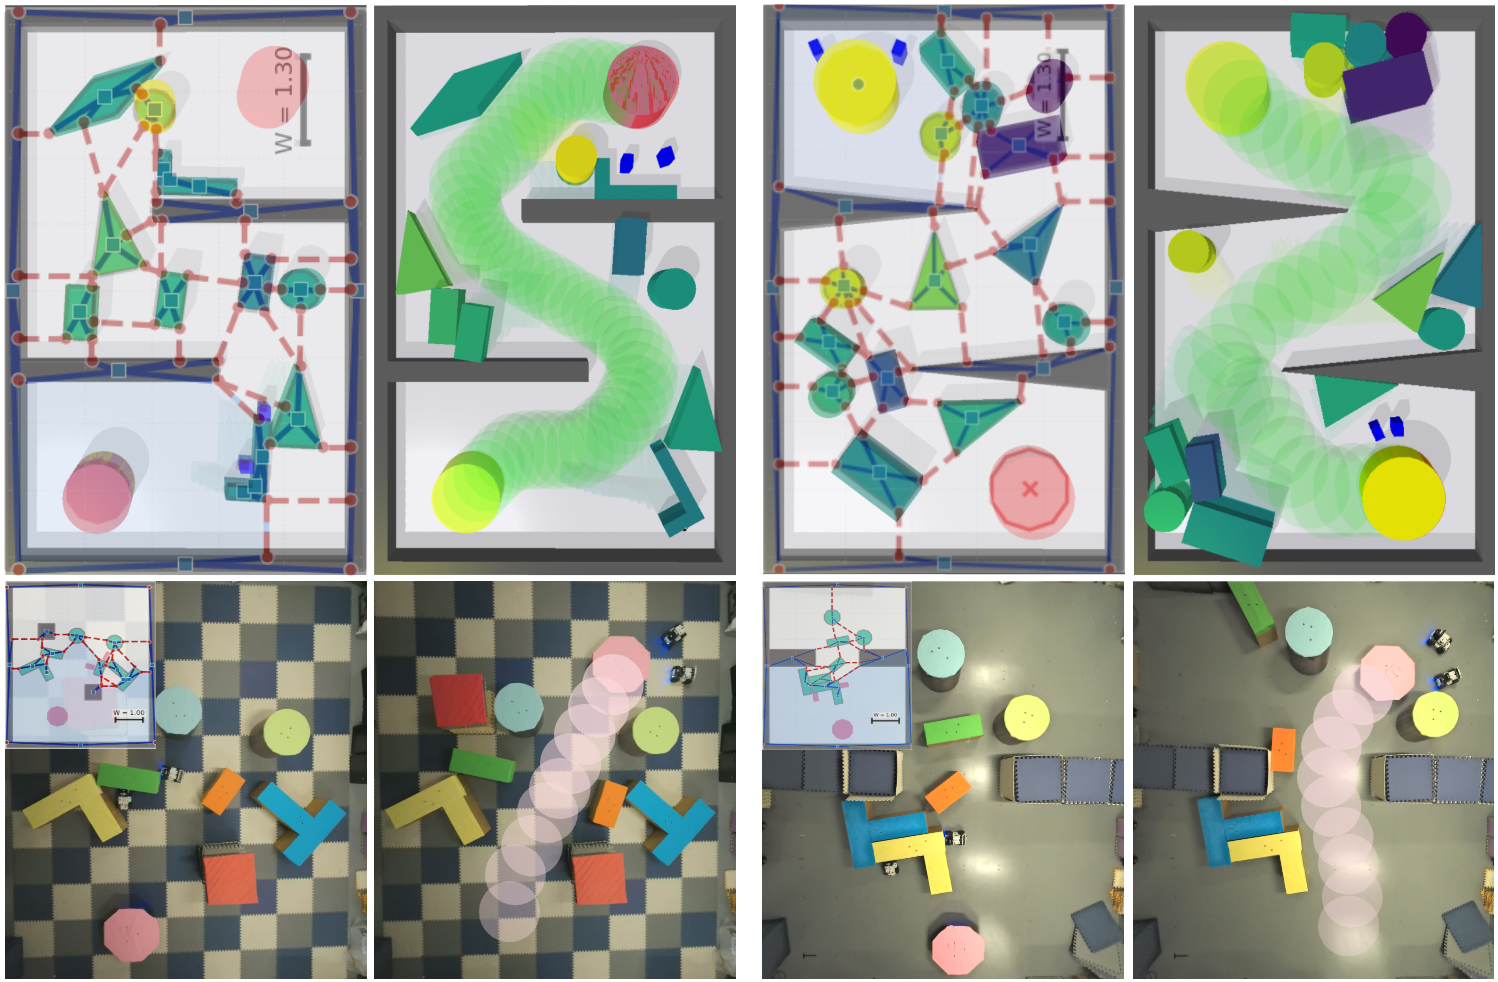
\includegraphics[width=0.9\linewidth]{figures/cover.png}% or {presearch.pdf}
  \vspace{-0.1in}
  \caption{
    Collaborative path clearing in simulation (\textbf{Top})
    and hardware (\textbf{Bottom}). Two robots push movable obstacles to
    create a $W$--clear path for a large vehicle from start to goal.
  }
  \vspace{-6mm}
  \label{fig:snapshots}
\end{figure}

%==============================================

\subsection{Related Work}\label{subsec:intro-related}

\looseness=-1
NAMO extends motion planning to cluttered environments by planning obstacle
displacements through pushing, pulling, or
rotating~\cite{stilman2005navigation,stilman2007manipulation}. Later work considers heuristic search, learning-based local planning, physics-based rollouts, and collaborative pushing~\cite{stilman2007manipulation,yao2024local,ren2025search,weeda2025pushing,tang2026pushingbots}.



%==============================================
\begin{figure*}[t!]
  \centering
  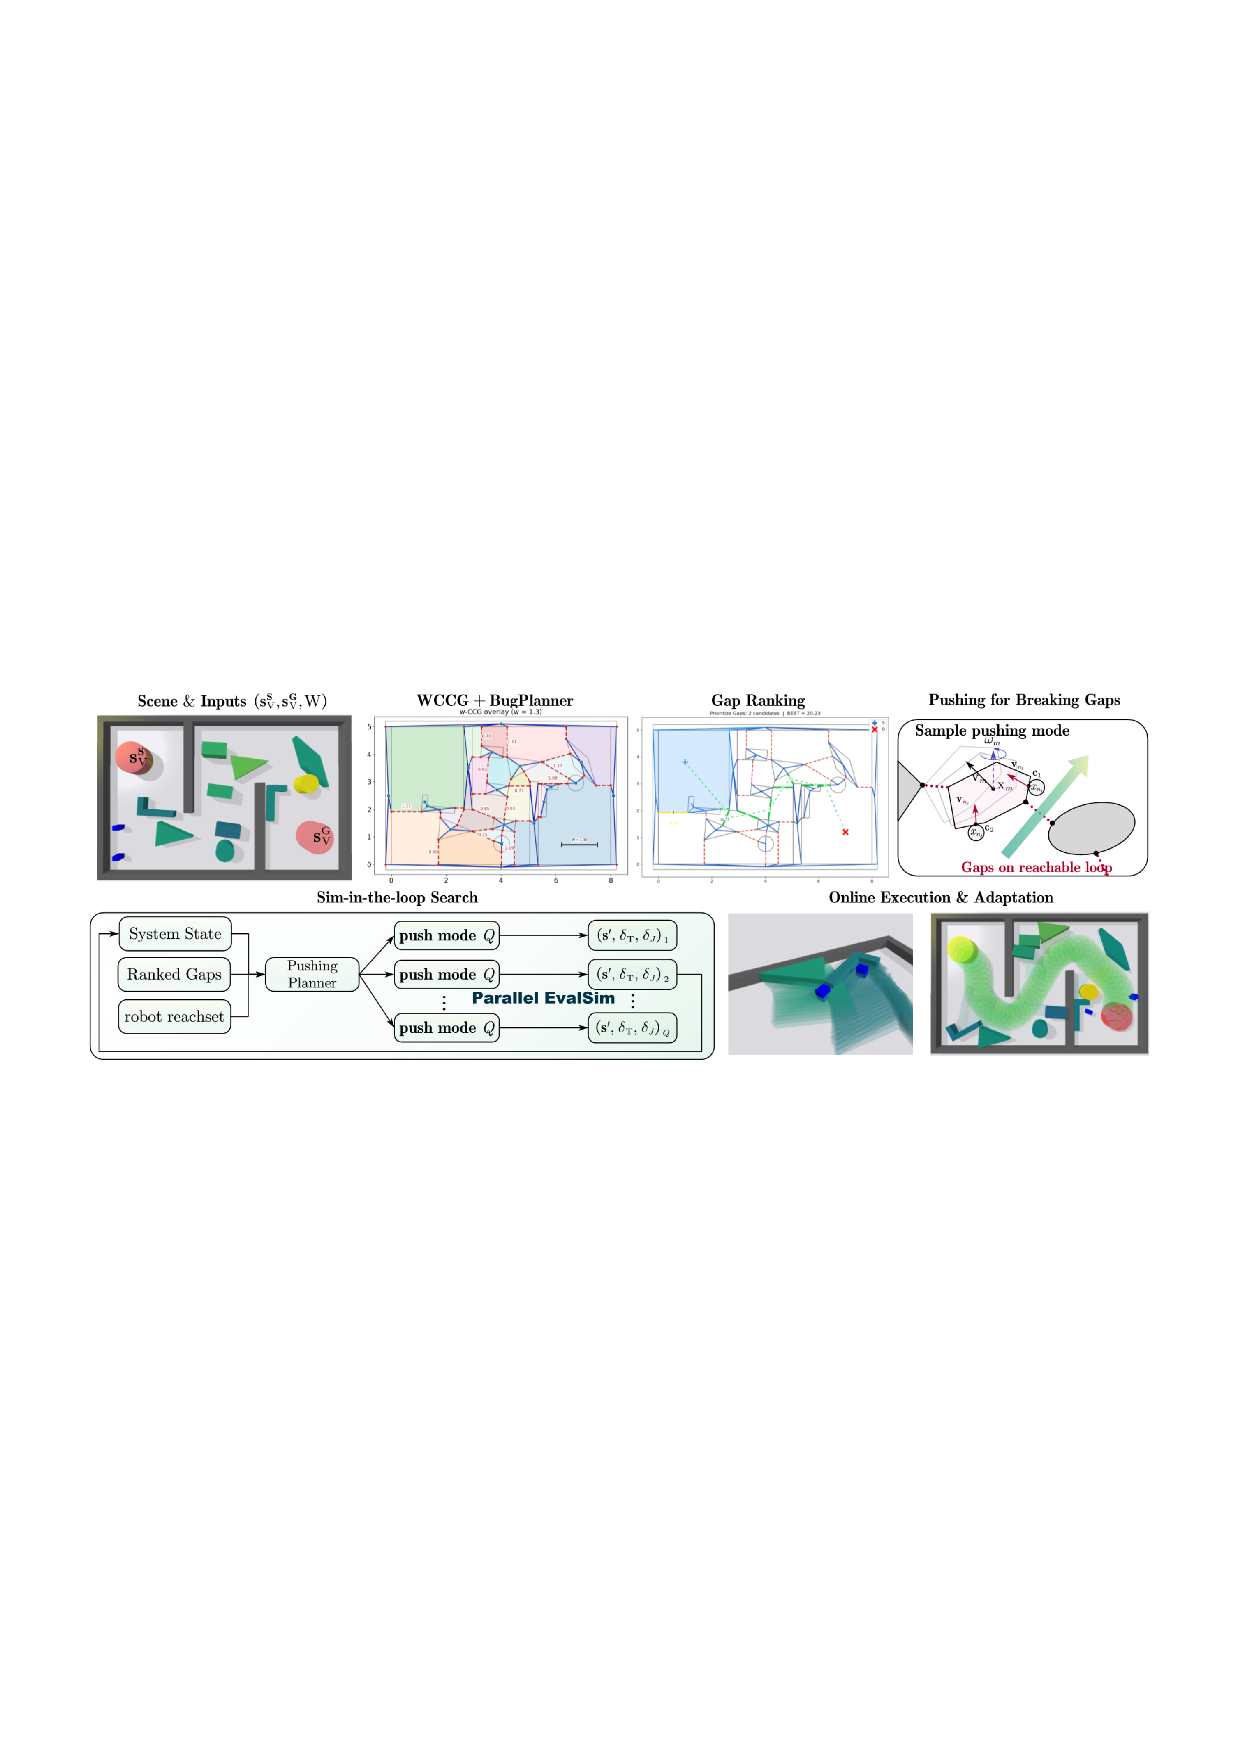
\includegraphics[width=0.84\linewidth]{figures/overall.pdf}
  \vspace{-0.1in}
\caption{Overview of the proposed framework.
\textbf{Top:} Scene inputs, WCCG construction, gap ranking, and sampling of pushing
modes for breaking frontier gaps;
\textbf{Bottom-left:} Sim-in-the-loop hybrid search with parallel validation in simulation;
\textbf{Bottom-right:} Online execution and adaptation during path clearing.}
  \label{fig:overall}
  \vspace{-5mm}
\end{figure*}
%==============================================


Collaborative pushing has been widely studied in multi-robot manipulation:
foundational work on the mechanics of pushing and limit surfaces~\cite{goyal1989limit,lynch1992manipulation}, cooperative transport with robot swarms~\cite{chen2015occlusion}, multi-robot box pushing with reinforcement learning~\cite{wang2006multi}, collaborative pushing of polytopic objects in cluttered scenes~\cite{tang2026pushingbots}, and learning-based loco-manipulation~\cite{feng2025learning}. These studies focus on a prescribed object rather than multi-object corridor clearing.

Physics-informed planning incorporates dynamics models, contact reasoning, or
simulation feedback into motion generation: learned dynamics for humanoid
contact planning~\cite{lin2019efficient}, multi-contact force control~\cite{rouxel2024multi}, demonstration-guided optimal control over contact modes~\cite{xue2023demonstration}, physics simulation interleaved with multi-agent pathfinding~\cite{saxena2023planning,ren2025object}, and learned physical priors~\cite{ni2023progressive,liu2025physics}. \change{These methods consider a prescribed target or few objects, whereas corridor clearing requires rearranging many obstacles to admit a larger vehicle.}


%==============================
\subsection{Our Method}\label{subsec:intro-our}

As shown in Fig.~\ref{fig:overall}, this work introduces \textbf{PushAround},
a physics-informed framework for collaborative multi-robot pushing that
constructs traversable corridors for large vehicles in cluttered environments.
Its central novelty is a hybrid search that jointly determines which obstacles
to displace and how to push them, coupling the high-level clearing sequence
with low-level pushing modes specifying contact points, directions and forces.
The framework integrates a W--clearance connectivity graph (WCCG) that certifies
vehicle passage under width constraints, frontier-gap ranking by estimated
effort, and pushing-mode generation under geometric and actuation constraints.
Guided by the selected gap, the search proposes direct pushes or recursively
clears blocking obstacles, and expands the plan through physics-validated
transitions that account for robot dimensions, object mass, contact geometry
and coupled pushing dynamics. Execution feedback updates connectivity and
triggers replanning when needed.
% \change{We further examine its robustness to physical-model uncertainty relevant to real-world deployment.}



The contributions are twofold: {(I)} it introduces a unified framework that
couples collaborative pushing with physics-informed verification, 
producing executable plans for path clearing in cluttered environments; 
and {(II)} \change{ 
it demonstrates empirical gains in feasibility, efficiency and scalability over evaluated NAMO and
collaborative-clearing baselines, with robustness to execution-side physics
mismatch.
}

%%========================================
\section{Problem Description}\label{sec:problem}
%==============================
\subsection{Workspace and Robots}\label{subsec:ws}
The workspace is a bounded planar region $\mathcal{W}\subset\mathbb{R}^2$
containing immovable structures~$\mathcal{O}\subset\mathcal{W}$ and $M\geq0$
movable rigid polygons
$\boldsymbol{\Omega}\triangleq\{\Omega_1,\cdots,\Omega_M\}\subset\mathcal{W}$.
Each movable obstacle~$\Omega_m$ has mass~$\mathsf{M}_m$,
inertia~$\mathsf{I}_m$, frictional parameters and state
$\mathbf{s}_m(t)\triangleq(\mathbf{x}_m(t),\psi_m(t))$, with
$\mathbf{x}_m(t)\in\mathbb{R}^2$ the centroid position and
$\psi_m(t)\in\mathbb{R}$ the orientation; $\Omega_m(t)$ denotes the region it
occupies at time~$t$. A team of~$N$ robots,
$\mathcal{R}\triangleq\{R_1,\cdots,R_N\}$, operates as a cooperative unit. Each
robot~$R_i$ is a rigid body with state
$\mathbf{s}_{R_i}(t)\triangleq(\mathbf{x}_{R_i}(t),\psi_{R_i}(t))$ and
footprint~$R_i(t)$. The instantaneous free space is given by:
\begin{equation}\label{eq:freespace}
\widehat{\mathcal{W}}(t)\triangleq\mathcal{W}\setminus\Big(
\mathcal{O}\cup\{\Omega_m(t)\}_{m=1}^{M}\cup\{R_i(t)\}_{i=1}^{N}
\Big),
\end{equation}
where~$\widehat{\mathcal{W}}(t)$ excludes regions occupied by immovable
obstacles, movable obstacles, and robots.

%==============================
\subsection{External Vehicle and Clearance Goal}\label{subsec:vehicle}
An external vehicle~$\texttt{V}$ whose footprint is enclosed by a disk of
radius~$W/2>0$ must navigate within the workspace from a start position
$\mathbf{x}_\texttt{V}^{\texttt{S}}\in\mathcal{W}$ to a goal position
$\mathbf{x}_\texttt{V}^{\texttt{G}}\in\mathcal{W}$. Since movable obstacles may
obstruct the way, the clearance goal is to rearrange them so that the workspace
contains a passage from~$\mathbf{x}_\texttt{V}^{\texttt{S}}$ to
$\mathbf{x}_\texttt{V}^{\texttt{G}}$ that can accommodate this enclosing disk,
i.e., a passage of width at least~$W$. At time~$t$, this is expressed by the
admissible reference-center space
$\mathcal{F}_W(t)\triangleq
\{p\in\widehat{\mathcal{W}}(t)\mid
\mathbb{B}_{W/2}(p)\subset\widehat{\mathcal{W}}(t)\}$, where
$\mathbb{B}_{W/2}(p)$ is the disk of radius~$W/2$ centered at~$p$. The
$W$-clearance condition is then given by:
\begin{equation}\label{eq:wclear}
\exists\,\mathcal{P}^W_\texttt{V}\subset\mathcal{F}_W(t):\
\mathbf{x}_\texttt{V}^{\texttt{S}}\leadsto\mathbf{x}_\texttt{V}^{\texttt{G}},
\end{equation}
which certifies a collision-free centerline path for any vehicle footprint
contained in the enclosing disk.
% Since movable obstacles may obstruct the way,
% a direct passage is not always feasible.
% At time~$t$, the admissible center positions of~$\texttt{V}$ are
% \begin{equation}
% \mathcal{F}_W(t)\triangleq
% \{p\in\widehat{\mathcal{W}}(t)\mid \mathbb{B}_{W/2}(p)\subset\widehat{\mathcal{W}}(t)\}.
% \end{equation}
% where $\mathbb{B}_{W/2}$ is a disk of radius~$W/2$.
% The clearance goal is satisfied if there exists a continuous centerline path
% inside~$\mathcal{F}_W(t)$:
% \begin{equation}\label{eq}
% \exists\,\mathcal{P}^W_\texttt{V}\subset\mathcal{F}_W(t):
% \mathbf{x}_\texttt{V}^{\texttt{S}}\leadsto\mathbf{x}_\texttt{V}^{\texttt{G}}.
% \end{equation}
% this therefore certifies a passage with width at
% least~$W$.


%==============================


\subsection{Collaborative Pushing Modes}\label{ss:interaction_mode}
To enlarge blocked gaps, the robots may actively
reconfigure~$\boldsymbol{\Omega}$ by pushing movable obstacles. For obstacle
$\Omega_m\in\boldsymbol{\Omega}$, a pushing mode is denoted by
$\boldsymbol{\xi}_m\triangleq(\mathbf{c}_m,\mathbf{u}_m)$, where
$\mathbf{c}_m=(c_1,\cdots,c_N)$ is an ordered tuple of contact points on
$\partial\Omega_m$, and the ordering specifies the robot-to-contact assignment.
The vector~$\mathbf{u}_m\in\mathbb{R}^{2N}$ stacks the corresponding planar
contact forces, expressed in the body frame of~$\Omega_m$; \change{an inactive
robot carries a null contact $c_i=\varnothing$ with zero force.}
For a contact tuple~$\mathbf{c}_m$, the set of admissible forces
${U}_m(\mathbf{c}_m)\subset\mathbb{R}^{2N}$ collects contact forces
satisfying the robot pushing limits, robot--object friction, and unilateral
contact constraints. The body wrench induced by a mode is defined as:
\begin{equation}
\mathbf{q}_m(\boldsymbol{\xi}_m)
\triangleq
G_m(\mathbf{c}_m)\mathbf{u}_m,
\label{eq:contact_wrench_map}
\end{equation}
where~$G_m(\mathbf{c}_m)\in\mathbb{R}^{3\times 2N}$ is the contact-to-wrench mapping;
and $\mathbf{q}_m(\boldsymbol{\xi}_m)\in\mathbb{R}^3$.
The admissible mode set is state dependent as denoted by~$\Xi_m(\mathbf{s})$.
It contains modes whose contacts are reachable from the
current robot configurations, pre-contact configurations are feasible in
the current clutter, and forces satisfy
$\mathbf{u}_m\in{U}_m(\mathbf{c}_m)$. Hence, applying a feasible
mode~$\boldsymbol{\xi}_m\in\Xi_m(\mathbf{s}(t))$ yields the physical
transition:
\begin{equation}\label{eq:transition}
  \mathbf{s}(t^+)\triangleq
  \Phi\big(\mathbf{s}(t),\,m,\,\boldsymbol{\xi}_m\big),
\end{equation}
where~$\mathbf{s}(t)$ stacks all robot and obstacle states.
\change{
The force vector~$\mathbf{u}_m$ serves as a feasibility variable to certify
wrench generation under the modeled contact and actuation constraints rather
than a directly commanded control input.
}


%==============================
\subsection{Problem Statement}\label{subsec:objective}

The goal is to compute a \emph{hybrid schedule} that reconfigures movable
obstacles to admit a $W$-feasible path for the external vehicle.
The schedule is defined as:
\begin{equation}\label{eq:schedule}
    \pi\triangleq
    \left\{
    \left(
    \Omega_{m_k},
    \mathbf{v}_k,
    \boldsymbol{\xi}_k
    \right)
    \right\}_{k=1}^{K},
\end{equation}
where~$\Omega_{m_k}\in\boldsymbol{\Omega}$ is the manipulated obstacle,
$\mathbf{v}_k$ its pushing direction, $\boldsymbol{\xi}_k\in\Xi_{m_k}$ its
pushing mode. The node cost is:
\begin{equation}\label{eq:problem}
    \mathcal{J}_{\mathrm{clr}}(\pi)
    \triangleq
    T+
    \alpha
    \sum_{k=1}^{K}
    J\left(
    m_k,\boldsymbol{\xi}_k,\mathbf{s}(t_k)
    \right),
\end{equation}
\change{where~$T\triangleq\sum_{k=1}^{K}\Delta t_k$ denotes 
the robotic clearance duration excluding vehicle traversal,  
with $\Delta t_k>0$ the duration that the evaluation in~(13) returns for the $k$-th push,
 and~$J(\cdot)$ is the simulation-estimated manipulation cost. 
 Vehicle traversal enters only through the terminal $W$-clearance condition~\eqref{eq:wclear}. 
 The constraints~\eqref{eq:freespace}--\eqref{eq:transition} 
 enforce valid pushing transitions. 
 Equation~\eqref{eq:problem} defines the realized clearance cost; PIHS samples finitely and does not guarantee optimality.}

% ==============================
\begin{remark}\label{remark:uniqueness}
  \change{The objective couples obstacle selection, pushing-mode generation and switching into one hybrid planning problem, yielding a combinatorial-continuous search space richer than classical NAMO formulations with hand-crafted contact modes~\cite{goyal1989limit,chen2015occlusion,wang2006multi}.}
  \hfill~$\blacksquare$
\end{remark}
% ==============================

%%========================================
% %% ========================================
\section{Proposed Solution}\label{sec:solution}

As shown in Figs.~\ref{fig:overall} and~\ref{fig:pihs_overview}, PushAround first
uses the W-Clearance
Connectivity Graph in Sec.~\ref{subsec:wccg} and gap ranking in
Sec.~\ref{subsec:gap} to identify and prioritize blocking gaps. It then
generates and evaluates physically feasible collaborative pushing modes in
Sec.~\ref{subsec:push}. These components are integrated into the
simulation-in-the-loop hybrid search of Sec.~\ref{subsec:simloop} and the online
execution procedure of Sec.~\ref{subsec:overall}.





% %% ========================================
%==============================================
\subsection{W--Clearance Connectivity Graph}\label{subsec:wccg}

The feasibility of routing the vehicle reduces to whether a~$W$-width corridor
connects~$\mathbf{x}_\texttt{V}^{\texttt{S}}$ and~$\mathbf{x}_\texttt{V}^{\texttt{G}}$.
A W--clearance connectivity graph (WCCG) is introduced here to encode obstacle
adjacencies under clearance~$W$ and enable fast connectivity queries.
\change{Conventional clearance checks either rasterize the workspace into an
inflated occupancy grid or query sampling-based roadmaps, and must therefore fix
a resolution and re-query the map whenever an obstacle
moves~\cite{karaman2011samplingbasedalgorithmsoptimalmotion}.
Built directly from obstacle geometry, the WCCG introduces no grid-resolution parameter in the repeated connectivity queries used during planning.}

%------------------------------
\begin{figure}[t!]
  \centering
  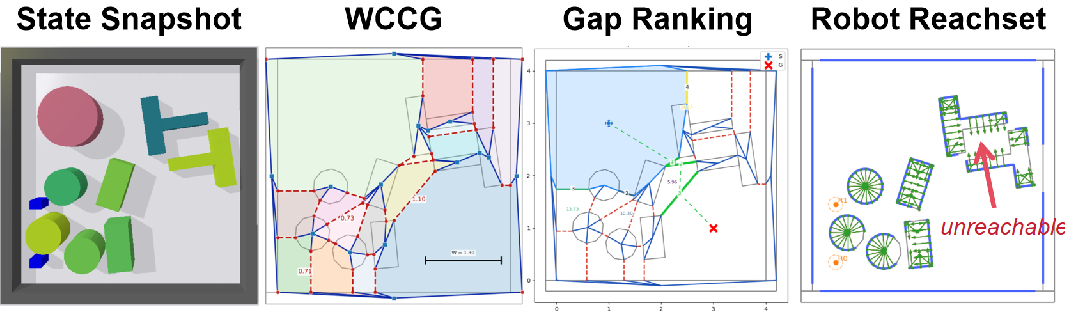
\includegraphics[width=0.9\linewidth]{figures/PIHS_top.pdf}
  \vspace{-2mm}
  \caption{\change{Core components of the physics-informed hybrid search: WCCG
  construction, gap ranking, mode generation, and physics validation.}}
  \label{fig:pihs_overview}
  \vspace{-4mm}
\end{figure}
%------------------------------

\subsubsection{Graph Construction}
The WCCG is built by decomposing all clearance-relevant obstacle and workspace
boundaries into convex components or segments.
From each component~$C$,
a centroid node~$v_c$ is created. When two components~$C_u$ and~$C_v$
have closest points~$p_u\in C_u$ and~$p_v\in C_v$ with distance less than~$W$,
bridge nodes are added at~$p_u$ and~$p_v$. These bridge nodes are
connected by a bridge--bridge edge, annotated with the gap width
$w_{uv}\triangleq\|p_u-p_v\|$, and further linked back to their centroids with
centroid--bridge edges. Narrow passages with~$w_{uv}<W$ are marked
as potential bottlenecks. The resulting graph is given by:
\begin{equation}\label{eq:wccg}
\mathcal{G}_W\triangleq(\mathcal{V},\; \mathcal{E}_c\cup\mathcal{E}_b),
\end{equation}
where~$\mathcal{V}$ are centroid and bridge nodes;
$\mathcal{E}_c$ contains centroid--bridge edges; and~$\mathcal{E}_b$ for
bridge--bridge edges with widths~$w_{uv}$.

\subsubsection{Connectivity Criterion}\label{subsubsec:bugplanner}
Once~$\mathcal{G}_W$ has been constructed, connectivity queries can be
performed without explicitly computing a geometric path. Let
$\textsf{Face}(\mathcal{G}_W)$ denote the set of connected planar faces induced
by the embedded WCCG, i.e., the maximal regions separated by obstacle
components and WCCG bottleneck edges. The criterion for~\eqref{eq:wclear}
is given by:
\begin{equation}\label{eq:wccg_criterion}
\big(\mathbf{x}_\texttt{V}^{\texttt{S}},\mathbf{x}_\texttt{V}^{\texttt{G}}\in
\mathcal{F}_W(t)\big)
\wedge
\big( \exists F\in\textsf{Face}(\mathcal{G}_W):
{\mathbf{x}_\texttt{V}^{\texttt{S}},\mathbf{x}_\texttt{V}^{\texttt{G}}}\in F \big)
\end{equation}
\change{The criterion follows the standard configuration-space inflation interpretation: 
expanding obstacles by a disk of radius $W/2$ turns gaps narrower than $W$ into overlapping barriers. 
Non-convex obstacles are handled through clearance-relevant decomposition, 
after which WCCG records the separating bottlenecks.
The consistency between WCCG connectivity and continuous and
rasterized configuration-space references is further evaluated numerically
in Sec.~\ref{subsec:wccg-validation}}.
A frontier-tracing procedure, similar to the
BugPlanner~\cite{McGuireCroonTuyls2019}, is then used to extract a skeleton
$\Sigma$ as an ordered sequence of centroid and bridge nodes. Starting from
$\mathbf{x}_\texttt{V}^{\texttt{S}}$, it casts a ray toward
$\mathbf{x}_\texttt{V}^{\texttt{G}}$ and follows the encountered frontier loop
until either a valid exit is found or a blocking cycle is returned.








%% \begin{algorithm}[t!]
%% \small
%% \caption{BugPlanner for~$W$-width connectivity (skeleton witness)}
%% \label{alg:bugplanner}
%% \DontPrintSemicolon
%% \SetKwInOut{Input}{In}\SetKwInOut{Output}{Out}
%% \Input{$\mathbf{s}^{\texttt{S}}$,~$\mathbf{s}^{\texttt{G}}$, WCCG}
%% \Output{if connected: skeleton~$\Sigma$; else: frontier loop~$\mathcal{L}$}
%%~$P\leftarrow\mathbf{s}^{\texttt{S}}$,~$\Sigma\leftarrow[\ ]$\;
%% \While{true}{
%%   \If{segment~$P\mathbf{s}^{\texttt{G}}$ hits no edge}{\Return~$\Sigma \cup \{\texttt{straight}(P,\mathbf{s}^{\texttt{G}})\}$}
%%   Build loop~$\mathcal{L}$ by angle-follow from the hit edge; append traversed edges to~$\Sigma$\;
%%   \If{$\mathrm{parity}(\mathcal{L},\,\mathbf{s}^{\texttt{S}}\mathbf{s}^{\texttt{G}})$ is odd}{\Return~$(\emptyset,\mathcal{L})$}
%%   Choose exit~$e$ on~$\mathcal{L}$ (outward normal~$\to\,\mathbf{s}^{\texttt{G}}$); append arc to~$\Sigma$;~$P\leftarrow e$ (tiny bias)\;
%% }
%% \end{algorithm}

% %% ========================================
%==============================================
\subsection{Ranking of Frontier Gaps}\label{subsec:gap}

When the condition in~\eqref{eq:wccg_criterion} fails, the vehicle cannot
reach~$\mathbf{x}_\texttt{V}^{\texttt{G}}$ from
$\mathbf{x}_\texttt{V}^{\texttt{S}}$ through a~$W$--clear path
$\mathcal{P}^W_\texttt{V}$.
In this case, the planner must prioritize
\emph{blocking gaps} on the reachable frontier of~$\mathcal{G}_W$
according to their predicted downstream cost, and feed the ranked list to the
hybrid search as local clearance targets.

\subsubsection{Frontier Extraction and Candidate Gaps}
A BugPlanner query on~$\mathcal{G}_W$ above
either confirms connectivity or returns a counter--clockwise frontier loop
$\mathcal{L}$ that separates the two endpoints. The bridge--bridge edges on
$\mathcal{L}$ define the first--hop candidate set
$\Gamma_\mathcal{L}\triangleq\{g_1,\cdots,g_K\}$,
where each gap~$g_k$ is represented by its two closest boundary points, its
width~$w_{g_k}<W$, and the adjacent obstacles that can potentially be moved.
These candidates are then ranked by predicted downstream cost and passed to the
hybrid search as local clearance targets.

\subsubsection{Evaluation for Immediate Cost}
Each candidate~$g\in\Gamma_\mathcal{L}$ is evaluated by combining the
cost for the robots to reach the gap and the effort required to widen it.
Let~$\mathbf{s}_{\mathcal{R}}$ be the current robot positions,
and~$\mathbf{o}_g$ as the outside insertion point of gap~$g$. The
resulting one--hop cost is given by:
\begin{equation}\label{eq:step_cost}
\mathsf{C}\big(g \mid \mathcal{L}, \mathbf{s}_{\mathcal{R}}\big)
=\lambda_\texttt{t}\,\mathsf{C}_\texttt{t}\!\left(\mathbf{s}_{\mathcal{R}},\mathbf{o}_g\right)
+\lambda_\texttt{p}\,\big( \mathsf{C}_\texttt{dp}(g) + \mathsf{C}_\texttt{rp}(g)\big)
\end{equation}
where~$\lambda_\texttt{t},\lambda_\texttt{p}>0$ weight the costs and $\mathsf{C}_\texttt{t}$, $\mathsf{C}_\texttt{dp}$, $\mathsf{C}_\texttt{rp}$ are the transition, direct and recursive terms.

%------------------------------
\begin{figure}[t!]
  \centering
  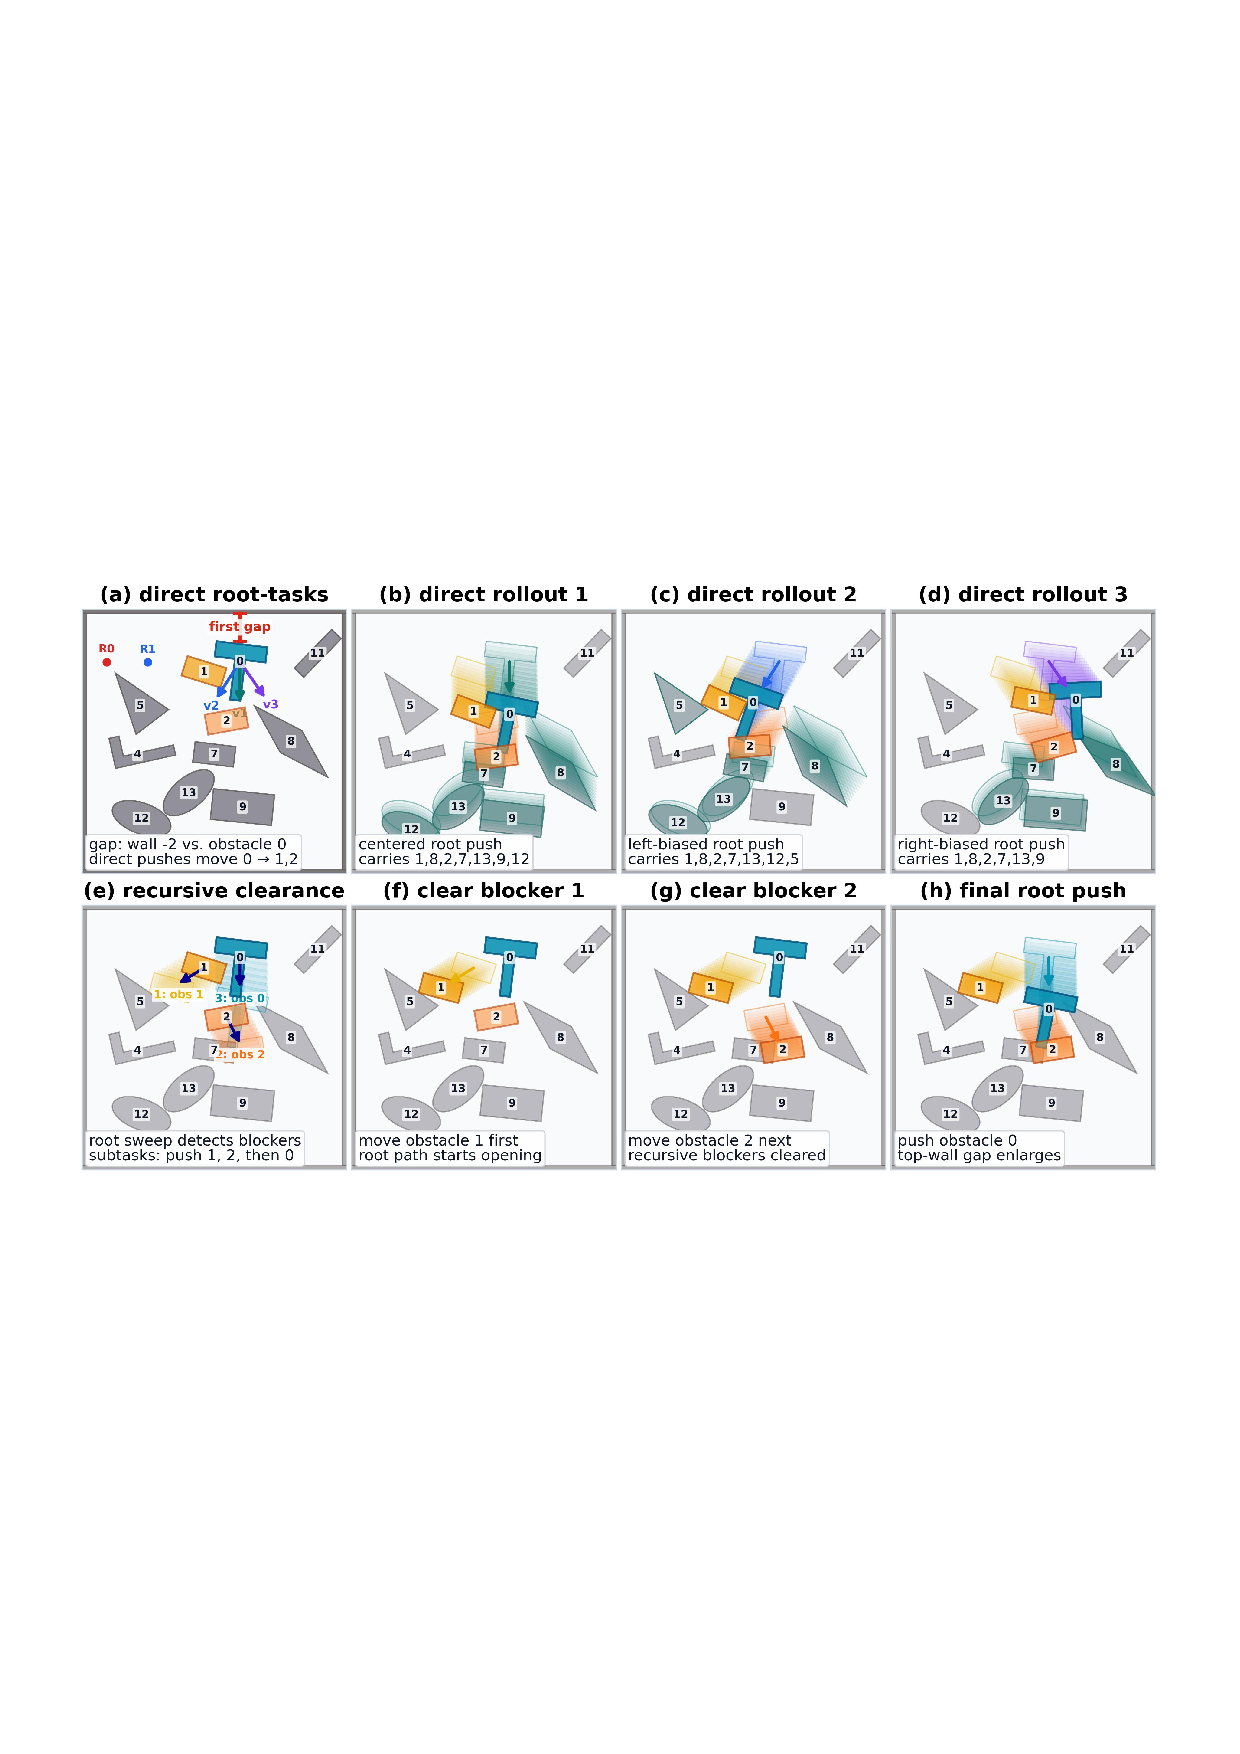
\includegraphics[width=0.85\linewidth]{figures/direct_recursive_push.pdf}
  \vspace{-0.1in}
  \caption{\change{
  \textbf{Direct} pushing moves a gap-side blocker along a gap-opening direction,
  whereas \textbf{recursive} pushing first clears movable blockers in the swept
  region and then returns to the root gap-opening task.}}
  \label{fig:direct_recursive_push}
  \vspace{-4mm}
\end{figure}

%------------------------------

\subsubsection{Long-term Cost w.r.t. Goal}
Furthermore, to prioritize gaps closer to the goal, a heuristic is added to the evaluation,
i.e.,
$h(g)=\eta\,\big\|\mathbf{o}(g)-\mathbf{x}_\texttt{V}^{\texttt{G}}\big\|$,
with the scaling constant~$\eta>0$.
Lastly, a short A$^\star$-style presearch is adopted to cross
each candidate gap, recompute the next frontier, and continue for a limited
width and depth. The \emph{cost-to-connect} is predicted by:
\begin{equation}\label{eq:pred_cost}
\widehat{\mathsf{Cost}}(g)\triangleq
\mathsf{C}\!\big(g \mid \mathcal{L},\mathbf{s}_{\mathcal{R}}\big)
+\!\!\!\sum_{g'\in\Pi^\star(g)}\!\!\!\big{\{}\mathsf{C}(g' \mid \cdot)+h(g')\big{\}},
\end{equation}
where~$\Pi^\star(g)$ is the sequence of subsequent gaps discovered after virtually crossing~$g$. Consequently, the final output of this module is the ranked list of candidate gaps, i.e.,
$\textsf{Rank}\big(\Gamma_\mathcal{L}\big)
\triangleq \textbf{argsort}_{g\in\Gamma_\mathcal{L}}\widehat{\mathsf{Cost}}(g)$,
in ascending predicted cost. This
ordered set is passed to the hybrid search module, such that only the
promising gaps are expanded first.



% %% ========================================
%==============================================
\subsection{Pushing Mode Generation and Evaluation}\label{subsec:push}
For a selected frontier gap~$g$, this subsection constructs candidate
pushing strategies
$\Xi_g\triangleq\{(\Omega_m,\mathbf{v},\boldsymbol{\xi})\}$,
where $\mathbf{v}=(v_x,v_y,\omega)\in\mathbb{R}^3$ is a short-horizon pushing
direction for~$\Omega_m$, and $\boldsymbol{\xi}=(\mathbf{c}_m,\mathbf{u})$
is its mode in~\eqref{eq:transition}.
\change{Wrench feasibility screens contact configurations that can realize
the required motion within actuation limits. The forces certify feasibility
rather than serving as hardware setpoints; candidate motion is then checked
by rollout or quick-pass reuse.}



%==============================================
\subsubsection{Direct and Recursive Pushing Tasks}
For \emph{direct push}, let~$\Omega_m$ denote one of the two movable obstacles adjacent to~$g$. For
each such obstacle, a small set of candidate body velocities
$\{\mathbf{v}_m^k\}_{k=1}^{K_m}$ is sampled with a bias toward enlarging the
gap~$g$, while a few angular components are included to account for local
geometry. If the swept region of a direct push intersects movable blockers,
\emph{recursive push} tasks are required instead: for each out-layer
blocker~$\Omega_m$, the nominal direction moves it away from both the swept
region and the reference gap sequence~$\Pi^\star(g)$. Recursion therefore
creates a bounded dependency chain which prioritizes the final
blocker~$\Omega_m$, as shown in Fig.~\ref{fig:direct_recursive_push}.






%==============================================
% \subsubsection{Pushing Mode Generation}
% For each sampled direction~$\mathbf{v}_m^k$ and obstacle~$\Omega_m$, the
% quality of a candidate mode is measured in the body frame. Let
% $\mathbf{v}_m^{k,\mathrm{B}} \in \mathbb{R}^3$ denote~$\mathbf{v}_m^k$
% expressed in the body frame of~$\Omega_m$. For a mode~$\boldsymbol{\xi}$,
% define the primary and multi-directional feasibility losses by:
% \begin{equation}\label{eq:mode-feasibility}
% \begin{aligned}
%   \mathrm{J}_{\texttt{F}}^m
%   (\boldsymbol{\xi},\mathbf{v}_m^{k,\mathrm{B}})
%   &\triangleq
%   \underset{\mathbf{q}_{m,\boldsymbol{\xi}} \in
%   \mathrm{Q}_{m,\boldsymbol{\xi}}}{\textbf{min}}
%   \left\|
%   \mathbf{q}_{m,\boldsymbol{\xi}} +
%   Q_\mu^m(\mathbf{v}_m^{k,\mathrm{B}})
%   \right\|_1,\\
%   \mathrm{J}_{\texttt{MF}}^m
%   (\boldsymbol{\xi},\mathbf{v}_m^{k,\mathrm{B}})
%   &\triangleq
%   \sum_{\mathbf{v}_d \in \mathcal{D}} w_d \cdot
%   \mathrm{J}_{\texttt{F}}^m(\boldsymbol{\xi},\mathbf{v}_d);
% \end{aligned}
% \end{equation}
% where~$\mathbf{q}_{m,\boldsymbol{\xi}} \in \mathbb{R}^3$ is the generalized
% body wrench induced by mode~$\boldsymbol{\xi}$;
% $\mathrm{Q}_{m,\boldsymbol{\xi}} \subseteq \mathbb{R}^3$ is the corresponding
% set of admissible body wrenches under the contact and friction constraints;
% $Q_\mu^m(\mathbf{v}_m^{k,\mathrm{B}}) \in \mathbb{R}^3$ denotes the
% quasi-static friction wrench of~$\Omega_m$ at direction~$\mathbf{v}_m^{k,\mathrm{B}}$;
% $\mathcal{D} \subset \mathbb{R}^3$ is a finite
% set of basis velocities containing the desired direction;
% and~$w_d > 0$ is the
% weight associated with~$\mathbf{v}_d \in \mathcal{D}$. Thus,
% small~$\mathrm{J}_{\texttt{F}}^m(\boldsymbol{\xi},\mathbf{v}_m^{k,\mathrm{B}})$ is
% necessary for force feasibility, while small
% $\mathrm{J}_{\texttt{MF}}^m$ indicates a robust mode.
% Accordingly, the associated mode
% $\boldsymbol{\xi}_m^k \triangleq (\mathbf{c}_m^k,\mathbf{u}_m^k)$ is generated
% by sparse optimization over the reachable part of~$\partial\Omega_m$. The
% reachable boundary is discretized into candidate contacts, and a sparse linear
% program (LP) is solved to minimize
% $\mathrm{J}_{\texttt{MF}}^m(\boldsymbol{\xi},\mathbf{v}_m^{k,\mathrm{B}})$
% under the local friction and wrench constraints.
% Detailed derivations are omitted here for brevity,
% and referred to~\cite{tang2024collaborative,tang2025pushingbots}.
% The resulting nonzero contacts provide~$\mathbf{c}_m^k$, and the corresponding forces
% yield~$\mathbf{u}_m^k$. Only the best few
% pairs~$(\mathbf{v}_m^k,\boldsymbol{\xi}_m^k)$ are retained and collected
% into~$\Xi_g$.

\subsubsection{Pushing Mode Generation}
At a search state~$\mathbf{s}$, a pushing mode is generated for each candidate
direction~$\mathbf{v}_m^k$ and obstacle~$\Omega_m$. In this subsubsection,
contact tuples, object velocities, forces, and wrenches are expressed in the
body frame of~$\Omega_m$. For a contact tuple~$\mathbf{c}$, its
multi-directional force feasibility is:
\begin{equation}\label{eq:mode-feasibility}
\mathrm{J}_{\texttt{MF}}^m(\mathbf{c},\mathbf{v}_m^k)
\triangleq
\sum_{\mathbf{v}_d\in\mathcal{D}_m^k} w_d
\underset{\mathbf{u}\in{U}_m(\mathbf{c})}{\textbf{min}}
\|
\mathbf{q}_m(\mathbf{c},\mathbf{u})
+\mathbf{q}_m^\mu(\mathbf{v}_d)
\| ,
\end{equation}
where~$\|\cdot\|$ is a weighted $\ell_1$ wrench norm, the finite set
$\mathcal{D}_m^k$ perturbs~$\mathbf{v}_m^k$, and
$\mathbf{q}_m^\mu(\mathbf{v}_d)$ is the quasi-static friction wrench; the inner
minimization is a small LP over the admissible forces ${U}_m(\mathbf{c})$.
A state- and direction-dependent contact set
$\mathcal{A}_m^k(\mathbf{s})\subset\partial\Omega_m$ is drawn from the
robot-reachable boundary of~$\Omega_m$ by velocity--force compatibility
filtering (Fig.~\ref{fig:mode_generation}), keeping a contact only if its
robots reach collision-free pre-contact poses. Starting from cached layouts or
random initializations, the tuple is refined by sequential greedy replacement:
at step~$\ell$, let $\mathbf{c}_{r,c}^{\ell}$ replace contact~$r$
with~$c$; select:
\begin{equation}
c^\star
=
\underset{c\in\mathcal{A}_m^k(\mathbf{s})}{\textbf{argmin}}\;
\mathrm{J}_{\texttt{MF}}^m
\bigl(\mathbf{c}_{r,c}^{\ell},\mathbf{v}_m^k\bigr),
\label{eq:greedy_mode_update}
\end{equation}
swept over contact slots until $\mathrm{J}_{\texttt{MF}}^m$ no longer
decreases or a bounded evaluation budget is reached.
The best tuple over initializations gives
$\mathbf{c}_m^{k,\star}$, from which $\mathbf{u}_m^k$ follows from the inner
minimization in~\eqref{eq:mode-feasibility}, yielding
$\boldsymbol{\xi}_m^k=(\mathbf{c}_m^{k,\star},\mathbf{u}_m^k)$; each mode is
cached as a warm start. \change{If the sequential replacement cannot assign a
contact to every robot, a bounded backtracking search over robot--contact
combinations (with a bounded budget) attempts the full-team assignment. If no feasible full-team mode is found
within this budget, for instance on small faces or under the pairwise
pusher-clearance constraint, one robot is temporarily left inactive and the
assignment is repeated with the remaining team. Reduced-team modes
carry a ranking penalty, so a feasible full-team mode is preferred, and the
inactive robot returns for the next task.} The best few admissible pairs are kept for gap~$g$ and
passed to simulation; $\mathbf{u}_m^k$ certifies wrench feasibility while
hardware tracks the contact geometry from pose/velocity commands.

% The best refined mode over all initializations is denoted by
% $\boldsymbol{\xi}_m^k=(\mathbf{c}_m^k,\mathbf{u}_m^k)$.
% It is admitted only if its rollout is validated in simulation.
% Accepted modes are stored in a persistent \textsc{mode-cache},
% indexed by discretized shape, mass, available robot force, and pushing direction,
% and reused as warm starts.
%------------------------------
\begin{figure}[t!]
  \centering
  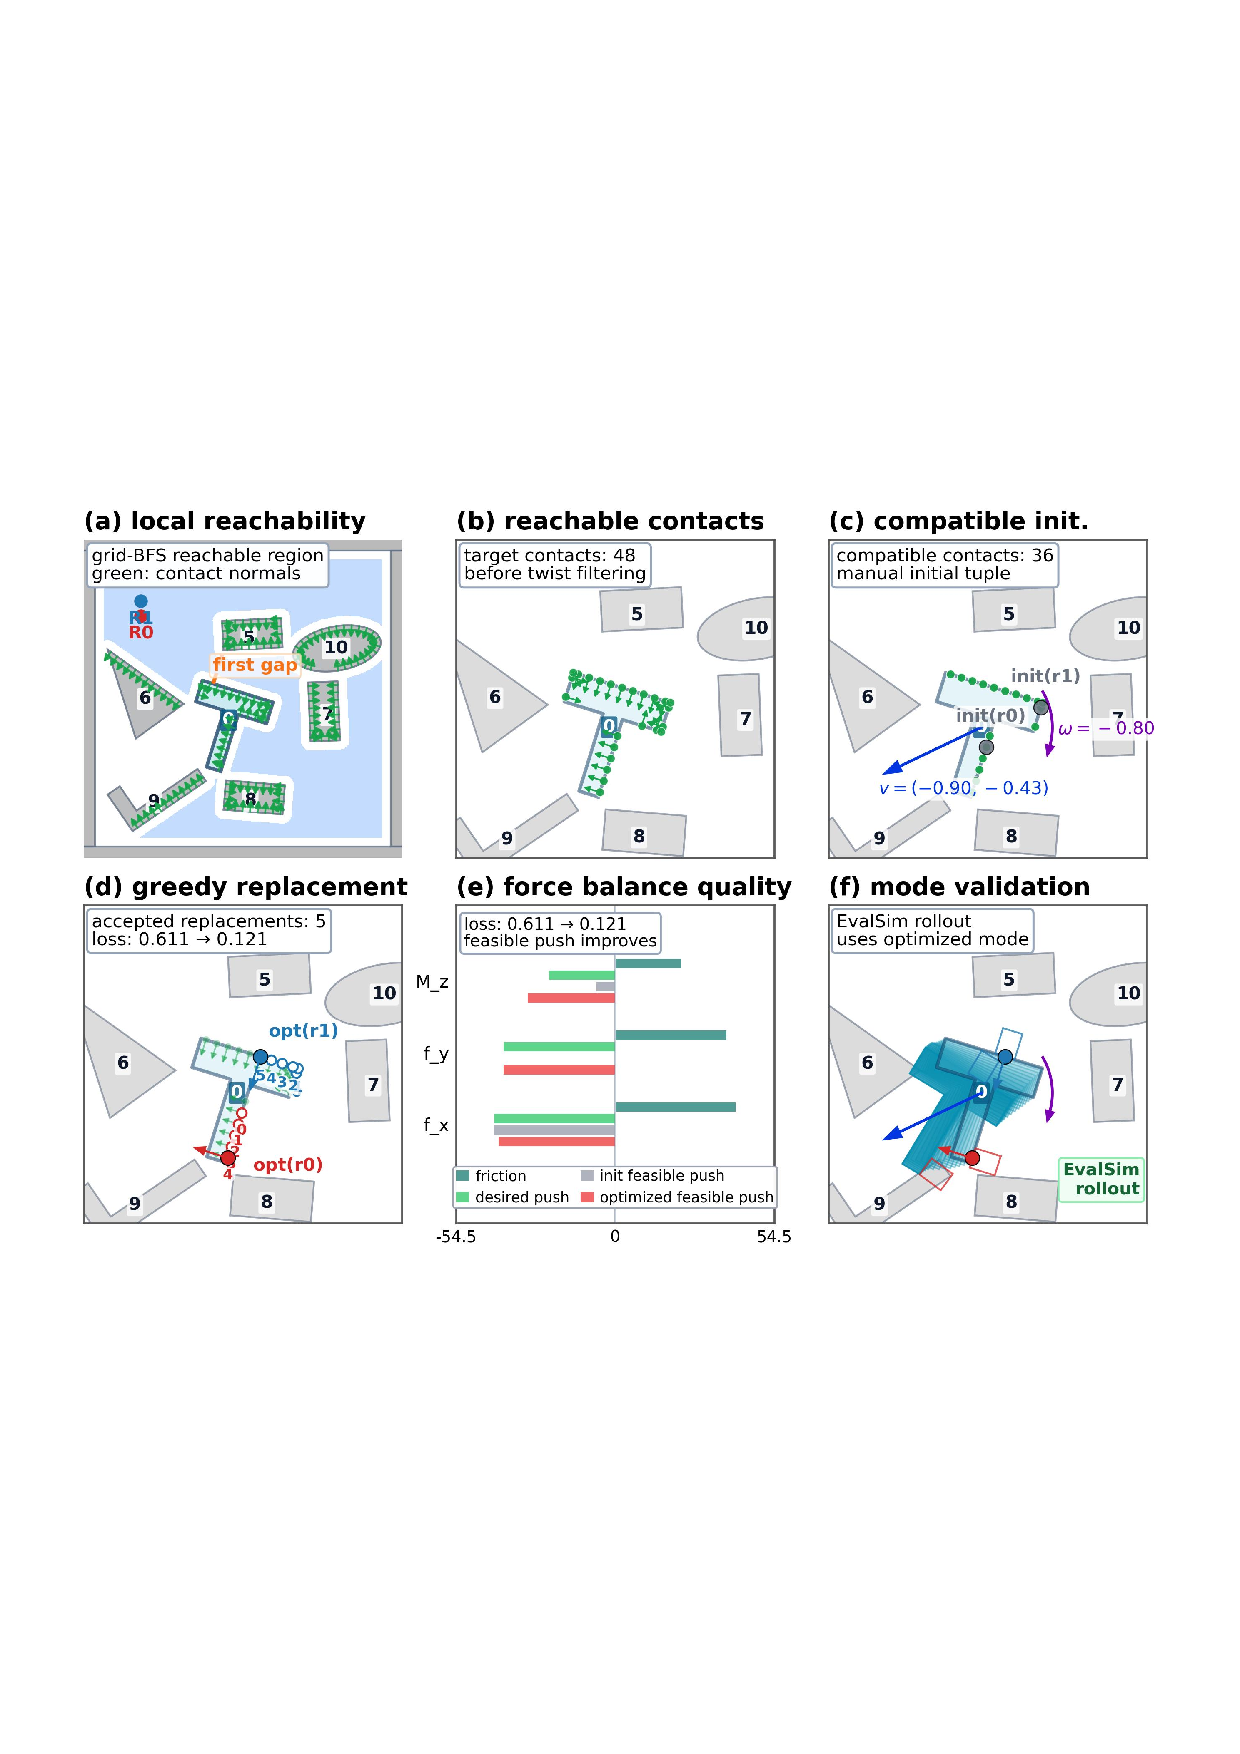
\includegraphics[width=0.85\linewidth]{figures/mode_generation.pdf}
  \vspace{-4mm}
  \caption{\change{Mode generation for a gap-opening task: (a) local reachability,
  (b) the reachable contact candidates after twist filtering, (c) a compatible
  initial contact tuple, (d) greedy replacement of individual contacts, (e) the
  force balance of the optimized push, and (f) rollout validation of the mode.}}
    \label{fig:mode_generation}
   \vspace{-4mm}
\end{figure}

%------------------------------
%==============================================
\subsubsection{Pushing Strategy Evaluation}

For a current state~$\mathbf{s}$ and candidate strategy
$(\Omega_m,\mathbf{v},\boldsymbol{\xi})\in\Xi_g$, a short-horizon rollout
evaluates the transition in~\eqref{eq:transition} under the selected mode.
As shown in Fig.~\ref{fig:mode_generation}, a strategy is accepted if the
robots reach the pre-contact poses, maintain stable contact and induce
obstacle motion above threshold. The simulation returns:
\begin{equation}
    (\mathbf{s}',\,\delta_{\texttt{T}},\,\delta_{\texttt{J}})
    \triangleq
    \mathsf{EvalSim}
    \big(
    \mathbf{s},(\Omega_m,\mathbf{v},\boldsymbol{\xi})
    \big),
    \label{eq:sim}
\end{equation}
where $\mathbf{s}'$ contains the resulting robot and object configurations,
$\delta_{\texttt{T}}>0$ is duration and $\delta_{\texttt{J}}$ control effort.
\change{Joint rollout captures contact-induced interactions among all bodies.
\minorchange{For quick-pass, a mode-table entry can store a validated body-frame state
sequence and cost increments. Under uniform, isotropic nominal dynamics,
translation invariance permits reuse for matching relative states, contacts,
twist, duration and physical properties (shape, mass, inertia, friction and
robot force limits), after reachability and robot--object swept-clearance
checks. Transforming the endpoint gives $\mathbf{s}'$ and cached increments
give $\delta_{\texttt{T}}$, $\delta_{\texttt{J}}$; uninvolved bodies remain
unchanged. Small parameter differences make reuse approximate.}}
%------------------------------
\begin{figure}[t!]
  \centering
  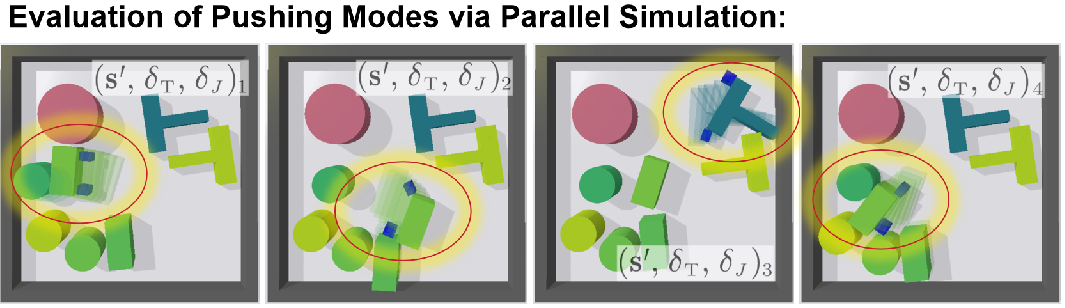
\includegraphics[width=0.95\linewidth]{figures/PIHS_bottom.pdf}
  \vspace{-2mm}
  \caption{\change{Sampled push tasks are evaluated via parallel simulation,
  producing updated states for search expansion.}}
    \label{fig:PIHS}
   \vspace{-4mm}
\end{figure}

%------------------------------

% %% ========================================
%==============================================
\subsection{Physics-Informed Hybrid Search}\label{subsec:simloop}

\change{The physics-informed hybrid search (PIHS) selects blocking gaps and
evaluates pushing strategies in parallel
(Fig.~\ref{fig:PIHS}, Alg.~\ref{alg:pihs}), \minorchange{using short-horizon simulation or
the nominal-model quick-pass reuse of Sec.~\ref{subsec:push}.}
Equation~\eqref{eq:problem} defines the evaluated clearance cost of a partial
schedule, used as the accumulated-cost term in the node priority
of~\eqref{eq:priority}.
Finite sampling gives no global optimality or completeness guarantee.}
\subsubsection{Tree and Initialization}
The search tree~$\mathcal{T}$ holds nodes
$\nu\triangleq(\mathbf{s},\pi)$, where~$\mathbf{s}$ is the system state of all
robots and movables in~\eqref{eq:transition} and~$\pi$ the partial pushing
strategy in~\eqref{eq:schedule}. Two global functions are maintained:
$\mathsf{Rank}(\nu)$ stores the ranked candidate
gaps~$\Gamma_{\mathcal{L}_\nu}$ of the frontier loop~$\mathcal{L}_\nu$ together
with their exploration costs by~\eqref{eq:pred_cost}, and~$\chi(\nu)$ returns
the cumulative execution cost from the root to~$\nu$. The root is
$\nu_0\triangleq(\mathbf{s}_0,\emptyset)$.
% At initialization,~$\chi(\nu_0)=0$, and
% $\mathsf{Rank}(\nu_0)$ is constructed by computing~$\Gamma_{\mathcal{L}_{\nu_0}}$
% for state~$\mathbf{s}_0$.

\subsubsection{Node Selection}
At each iteration, the node with minimum best-first priority is selected from
the queue. Priority balances realized cost and estimated remaining effort:
\begin{equation}\label{eq:priority}
  f(\nu)\triangleq \chi(\nu)+\underset{g\in \textsf{Rank}(\nu)}{\textbf{min}}
  \widehat{\mathsf{Cost}}(g),
\end{equation}
where~$\chi(\nu)$ is the cumulative execution cost so far, and the second term
is the minimum predicted remaining cost among the unexplored gaps of~$\nu$.
\change{The remaining-cost term is a heuristic and is not required to be admissible. The score prioritizes nodes by realized cost and promising future actions, but it does not provide an A* optimality guarantee.}



\begin{figure*}[t!]
  \centering
  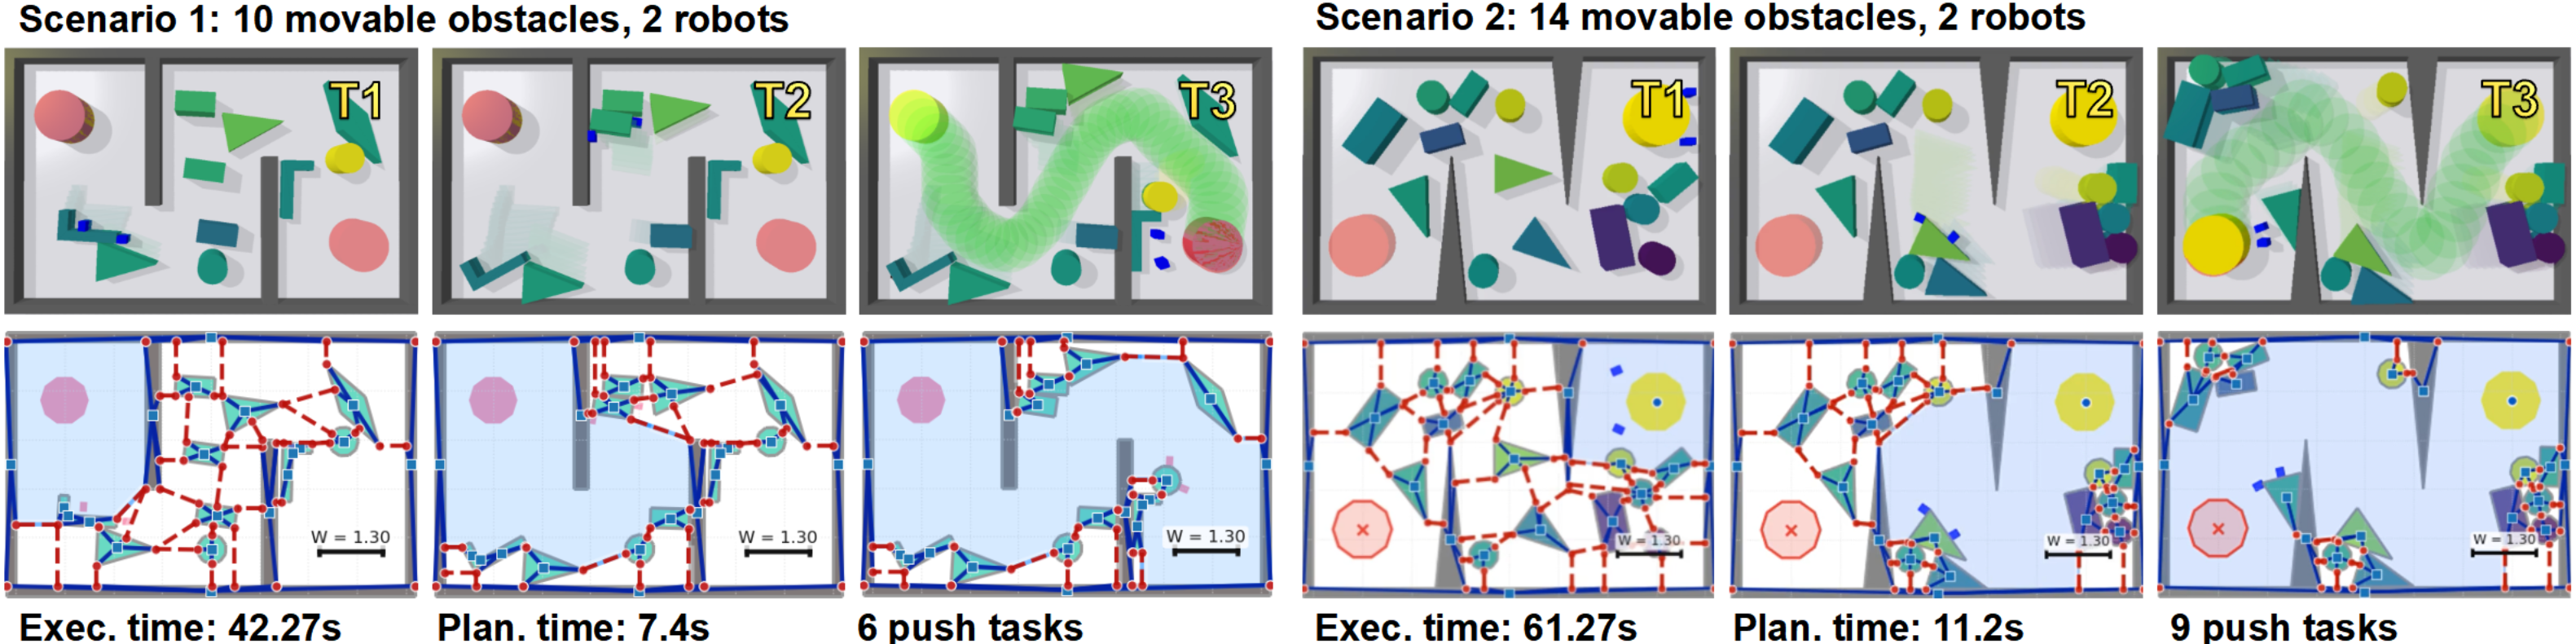
\includegraphics[width=0.95\linewidth]{figures/sim_fixed.png}
  \vspace{-2mm}
  \caption{\change{Execution and planning alignment in Scenario 1 (\textbf{Left})
    and  Scenario 2 (\textbf{Right}).
\textbf{Top:} simulated snapshots during path clearing.
\textbf{Bottom:} corresponding WCCG overlays with the start face in blue.
The executed pushes progressively expand the reachable $W$--clearance region until the goal is connected.}}
\vspace{-6mm}
\label{fig:main_result}
\end{figure*}
% ========================================

% ========================================
\subsubsection{Node Expansion with Parallel Simulation}
Let the selected node be~$\nu \triangleq (\mathbf{s},\pi)$. For each ranked gap
$g \in \mathsf{Rank}(\nu)$,
its predicted gap sequence~$\Pi^\star(g)$ in~\eqref{eq:pred_cost}
is first derived. Then, the mode optimization by~\eqref{eq:mode-feasibility}
provides a candidate strategy set
$\Xi_g \triangleq \{(\Omega_m,\mathbf{v},\boldsymbol{\xi})\}$,
including both the direct push of the adjacent movable obstacles,
and recursive push of out-layer obstacles.
Thus, expansion is prioritized first by the gap ordering in
$\mathsf{Rank}(\nu)$, and then by the candidate ordering within~$\Xi_g$.
\minorchange{Each candidate is evaluated by~\eqref{eq:sim}, using quick-pass reuse
or a rollout as described in Sec.~\ref{subsec:push}.}
A successful evaluation yields
$(\mathbf{s}',\delta_{\texttt{T}},\delta_{\texttt{J}})$, from which a child
node~$\nu' \triangleq (\mathbf{s}',\pi')$ is created with
$\pi' \triangleq \pi \cup \{\tau\}$, appending
$\tau \triangleq (\Omega_m,\mathbf{v},\boldsymbol{\xi})$ to the current partial
schedule~$\pi$.
The cumulative cost is updated by:
$\chi(\nu') \triangleq \chi(\nu) + \widehat{\mathsf{C}}(\nu,\tau)$,
where~$\widehat{\mathsf{C}}(\nu,\tau)\triangleq
\delta_{\texttt{T}} + \alpha\,\delta_{\texttt{J}}$
\change{is the evaluated incremental cost.}
Thereby, one expansion can yield several validated successors.


{
\SetAlFnt{\small}
\SetAlgoSkip{0pt}
%==============================================
\begin{algorithm}[t!]
\caption{Physics-Informed Hybrid Search}\label{alg:pihs}
\SetAlgoLined
\KwIn{$\mathbf{s}_0$,~$\alpha$,~$\mathsf{EvalSim}(\cdot)$,~$W$--criterion by~\eqref{eq:wccg_criterion}}
\KwOut{Clearing schedule $\pi^\star$, or failure}
$\nu_0\gets(\mathbf{s}_0,\emptyset),\;\chi(\nu_0)=0$\;
Init~$\mathcal{Q}$ by~\eqref{eq:priority}\;
\While{$\mathcal{Q}\ne\emptyset$ and budget remains}{
 $\nu=(\mathbf{s},\pi)\gets\mathcal{Q}.\texttt{pop\_min}()$ by~\eqref{eq:priority}\;
 \If{$\mathbf{s}$ admits~$\mathcal{P}^W_{\texttt{V}}$ by~\eqref{eq:wccg_criterion}}{
  \Return $\pi$\;
 }
  \ForEach{$g\in\mathsf{Rank}(\nu)$}{
    Compute~$\Pi^\star(g)$, generate~$\Xi_g$\;
    \ForEach{$(\Omega_m,\mathbf{v},\boldsymbol{\xi})\in\Xi_g$}{
      $\tau=(\Omega_m,\mathbf{v},\boldsymbol{\xi})$ \tcp{Direct or recur.}
      $(\mathbf{s}',\delta_\texttt{T},\delta_\texttt{J})\gets\mathsf{EvalSim}(\nu,\tau)$
      by~\eqref{eq:sim}\;
    \If{success}{
     $\pi'\gets\pi\cup\{\tau\}$\;
     $\nu'\gets(\mathbf{s}',\pi')$\;
     $\chi(\nu')\gets\chi(\nu)+\delta_\texttt{T}+\alpha\,\delta_\texttt{J}$\;
     Add $\nu'$ to $\mathcal{Q}$\;
      }
    }
  }
}
\Return failure;
\end{algorithm}
%==============================================
}
%==============================

\subsubsection{Termination}
Termination occurs when a node~$\nu$ reaches a state~$\mathbf{s}$ for which a
$W$--clear path~$\mathcal{P}^W_\texttt{V}$ exists from
$\mathbf{x}_\texttt{V}^{\texttt{S}}$ to~$\mathbf{x}_\texttt{V}^{\texttt{G}}$
by~\eqref{eq:wccg_criterion}. \change{Thus, $\pi$ encodes both the gaps to clear
and the strategies that realize them, satisfying nominal clearance and
evaluated pushing transitions. This does not imply global minimization
of~$\mathcal{J}_{\mathrm{clr}}$. The objective covers clearing only;
vehicle traversal follows afterwards.}

\begin{remark}\label{remark:simloop}
\change{Gap-lookahead reduces unproductive branches, \textsc{mode-cache}
warm-starts optimization, \minorchange{and quick-pass reuses validated transitions
to avoid redundant rollouts.}}
\hfill$\blacksquare$
\end{remark}

% %%========================================
%==============================
\subsection{Overall Analyses}\label{subsec:overall}

\subsubsection{Execution and Online Adaptation}\label{subsec:execute}
The hybrid search returns a pushing schedule
$\pi = \{\tau_1,\cdots,\tau_K\}$, with
$\tau_k \triangleq (\Omega_k,\mathbf{v}_k,\boldsymbol{\xi}_k)$.
The schedule is executed in a receding-horizon manner: for each $\tau_k$ the
robots reach the mode~$\boldsymbol{\xi}_k$ and follow the pushing
direction~$\mathbf{v}_k$ from the current state, as in~\eqref{eq:sim}.
\change{On the hardware the optimized contact forces certify feasibility rather
than being commanded: a mode is retained only if its object wrench lies within
the robots' actuation limits, and over each control interval $\mathsf{EvalSim}$ predicts a short forward
object-motion reference (the expected displacement and rotation of the object),
which the velocity-level controller tracks with motion-capture feedback, and each
executed push returns an observed state that re-enters the planner.} During transitions,
robots are reassigned by preserving the circular order of contact points along
the obstacle boundary~\cite{tang2026pushingbots}, reducing path crossings under
sufficient clearance. After each push the state is updated from observation,
the WCCG is rebuilt from the current configuration, and execution continues
until a $W$-clear path
$\mathcal{P}^W_\texttt{V}$ connects~$\mathbf{x}_\texttt{V}^{\texttt{S}}$ and
$\mathbf{x}_\texttt{V}^{\texttt{G}}$.
Replanning is triggered by observed execution discrepancies -- failed contact
establishment, stalled pushing, or invalidated WCCG connectivity -- in which
case Alg.~\ref{alg:pihs} is called from the current state to derive the
updated schedule.

%----------------------------------------------
\subsubsection{Computational Complexity}\label{subsubsec:complexity}

Given~$M$ movable obstacles, the computational cost of one node
expansion in Alg.~\ref{alg:pihs} is dominated by candidate generation and
physics validation. The WCCG update and gap ranking incur
$\mathcal{O}(M\log M+|\mathcal{V}|+|\mathcal{E}_c|+|\mathcal{E}_b|)$ and
$\mathcal{O}(|\Gamma_{\mathcal{L}_\nu}|
\log|\Gamma_{\mathcal{L}_\nu}|)$ costs, respectively.
\change{The dominant simulation cost
$\mathcal{O}\big(\sum_{g\in\mathsf{Rank}(\nu)}|\Xi_g|\,\big(C_{\mathrm{LP}}+\rho_\nu T_{\mathrm{sim}}/n_{\texttt{w}}\big)\big)$
grows with the number of validated candidates and is reduced by the
$n_{\texttt{w}}$ parallel workers, so scalability is set by validated
candidates rather than by the enumeration of contact assignments.} \change{Robot-team size mainly affects mode
generation: the greedy stage evaluates at most $N|\mathcal{A}|$ single-contact
substitutions instead of the exhaustive $|\mathcal{A}|^N$ assignment, and when it
fails, a bounded-backtracking search over robots and candidates expands at most
$B{=}2000$ partial assignments, a fixed budget independent of the team size; the
subset fallback repeats this search for at most one excluded robot. The number
of LP feasibility checks per task is therefore at most
$(N|\mathcal{A}|{+}2B)$, each over the $2N$ admissible contact forces, rather
than growing as $|\mathcal{A}|^N$.}
%% %----------------------------------------------
%% \subsubsection{Generalization}\label{subsec:general}
%% The framework admits several extensions:
%% (I) \textit{Heterogeneous teams.} Per-robot gain tuning and robot-specific mode
%% priors enable cooperation among diverse robots;
%% (II) \textit{Concurrent pushing.} Multi-object mode generation and conflict-aware
%% transition planning allow multiple obstacles to be pushed simultaneously;
%% (III) \textit{Dynamic environments.} Periodic $W$--connectivity checks and
%% on-demand replanning handle disturbances such as object drift or unmodeled
%% contacts during execution.

% %%========================================

%%========================================
% ============================================================
\section{Experiments}
\label{sec:experiments}
We evaluate PIHS in simulation and hardware (see accompanying video).
The algorithms are implemented in \texttt{Python3} and \texttt{PyBullet}~\cite{coumans2019}
on a machine with an Intel i9-14900KF and an RTX 4080.
\subsection{Numerical Simulations}
\label{subsec:sim}
% ========================================
\begin{table}[t]

\centering

\caption{\change{WCCG connectivity validation and mean runtime.}}

\label{tab:wccg-validation}

\vspace{-2.0mm}

\footnotesize

\setlength{\tabcolsep}{3.8pt}
\setlength{\belowrulesep}{0.30ex}
\renewcommand{\arraystretch}{0.86}

\change{
\begin{tabular}{
 @{}
 l
 cc
 @{\hspace{8pt}}
 ccc
 @{}
}

\toprule

&
\multicolumn{2}{c}{Validation}
&
\multicolumn{3}{c}{Runtime (ms)}
\\[-0.6ex]

\cmidrule(lr){2-3}
\cmidrule(lr){4-6}

Type
& CC $=$ FR
& FP/FN$^\dagger$
& CC
& FR
& WCCG
\\

\midrule

Convex
& 100/100
& 0/0
& 1.23
& 282.9
& \textbf{0.86}
\\

Non-convex
& 98/100
& 0/0
& 1.51
& 204.1
& \textbf{1.30}
\\

Mixed
& 98/100
& 0/0
& 1.33
& 242.4
& \textbf{1.05}
\\

\midrule

Total
& 296/300
& \textbf{0/0}
& 1.36
& 243.1
& \textbf{1.07}
\\

\bottomrule

\end{tabular}
}

\vspace{0.5mm}

{\scriptsize
\change{
$^\dagger$WCCG errors relative to the continuous configuration-space reference (CC).
All runtimes use the same 300-scene harness with the compiled WCCG backend.
}
}

\vspace{-5.5mm}

\end{table}

\subsubsection{Setup and Configuration}\label{subsec:sim-setup}

The simulation runs at a step size of $\Delta t=1/240$\,s with a control period
of $1/40$\,s; robots are disk or box pushers consistent with the $W$-clearance
definition, and movable obstacles have masses $[5,15]$\,kg in Scenarios~1--2, $[20,30]$\,kg in the generalization studies. A trial
succeeds when the external vehicle reaches its goal through a $W$-clear path. The
nominal scenario is an $8\times5$\,m workspace with bottleneck-forming bar
obstacles, where two robots clear $10$--$15$ movable obstacles under
minimum-separation constraints. Unless stated otherwise, comparisons and
ablations use Scenario~1 ($10$ movable obstacles, $40$ trials), and Scenario~2
($14$ obstacles) provides an additional cluttered case
(Fig.~\ref{fig:main_result}). \change{All methods share the robot footprints,
obstacle configurations, collision and reachability checks, and execution
simulator, with the same $800$\,s planning cap, $20{,}000$-step ($500$\,s) execution cap and $8$ workers. Unless stated otherwise, times average over successful trials, failures counting only in the success rate; the scalability curves instead cap failures.}



% ========================================
\begin{table}[t]
 \centering
 \begin{threeparttable}
 \caption{Performance comparison and ablations on Scenario~1 over $40$ randomized trials.\tnote{a}}
 \label{tab:main_ablation}
 \setlength{\tabcolsep}{2.7pt}
 \renewcommand{\arraystretch}{0.92}
 \begin{tabular}{lccccc}
 \toprule
 Method / Variant & Succ.(\%) & PT (s) & ET (s) & \#Sims & \#Pushes \\
 \midrule
 DFS-WCCG & 25.0 & $>$100.0 & 51.2 & $>$500 & 8.0 \\
 SL-Push (offline) & 62.5 & 0.06 & 44.1 & 0.0 & 7.3 \\
 SL-Push (sim) & 75.0 & 18.2 & 64.6 & 20.0 & 10.2 \\
 Rec-NAMO & 37.5 & 13.3 & 42.4 & 0.0 & 7.8 \\
 \textbf{PushAround (ours)}
 & \textbf{97.5} & \textbf{10.3} & \textbf{28.6}
 & \textbf{121.5} & \textbf{6.0} \\
 \midrule
 w/o gap-lookahead & 82.5 & 16.9 & 35.2 & 178.3 & 7.2 \\
 w/o mode-cache & 92.5 & 17.1 & 33.4 & 164.6 & 6.5 \\
 w/o quick-pass & 90.0 & 23.6 & 41.9 & 208.2 & 6.1 \\
 w/o reinsertion & 85.0 & 12.8 & 31.1 & 151.7 & 7.8 \\
 \bottomrule
 \end{tabular}
 \begin{tablenotes}\scriptsize
 \item[a] Times are averaged over successful trials; failures count in the
 success rate only. For DFS-WCCG, $PT$ and
 \#Sims are not comparable and are given as lower bounds ($>$).
 \end{tablenotes}
 \end{threeparttable}
 \vspace{-4.0mm}
\end{table}

% ========================================
% ========================================
\begin{figure}[t!]
 \centering
 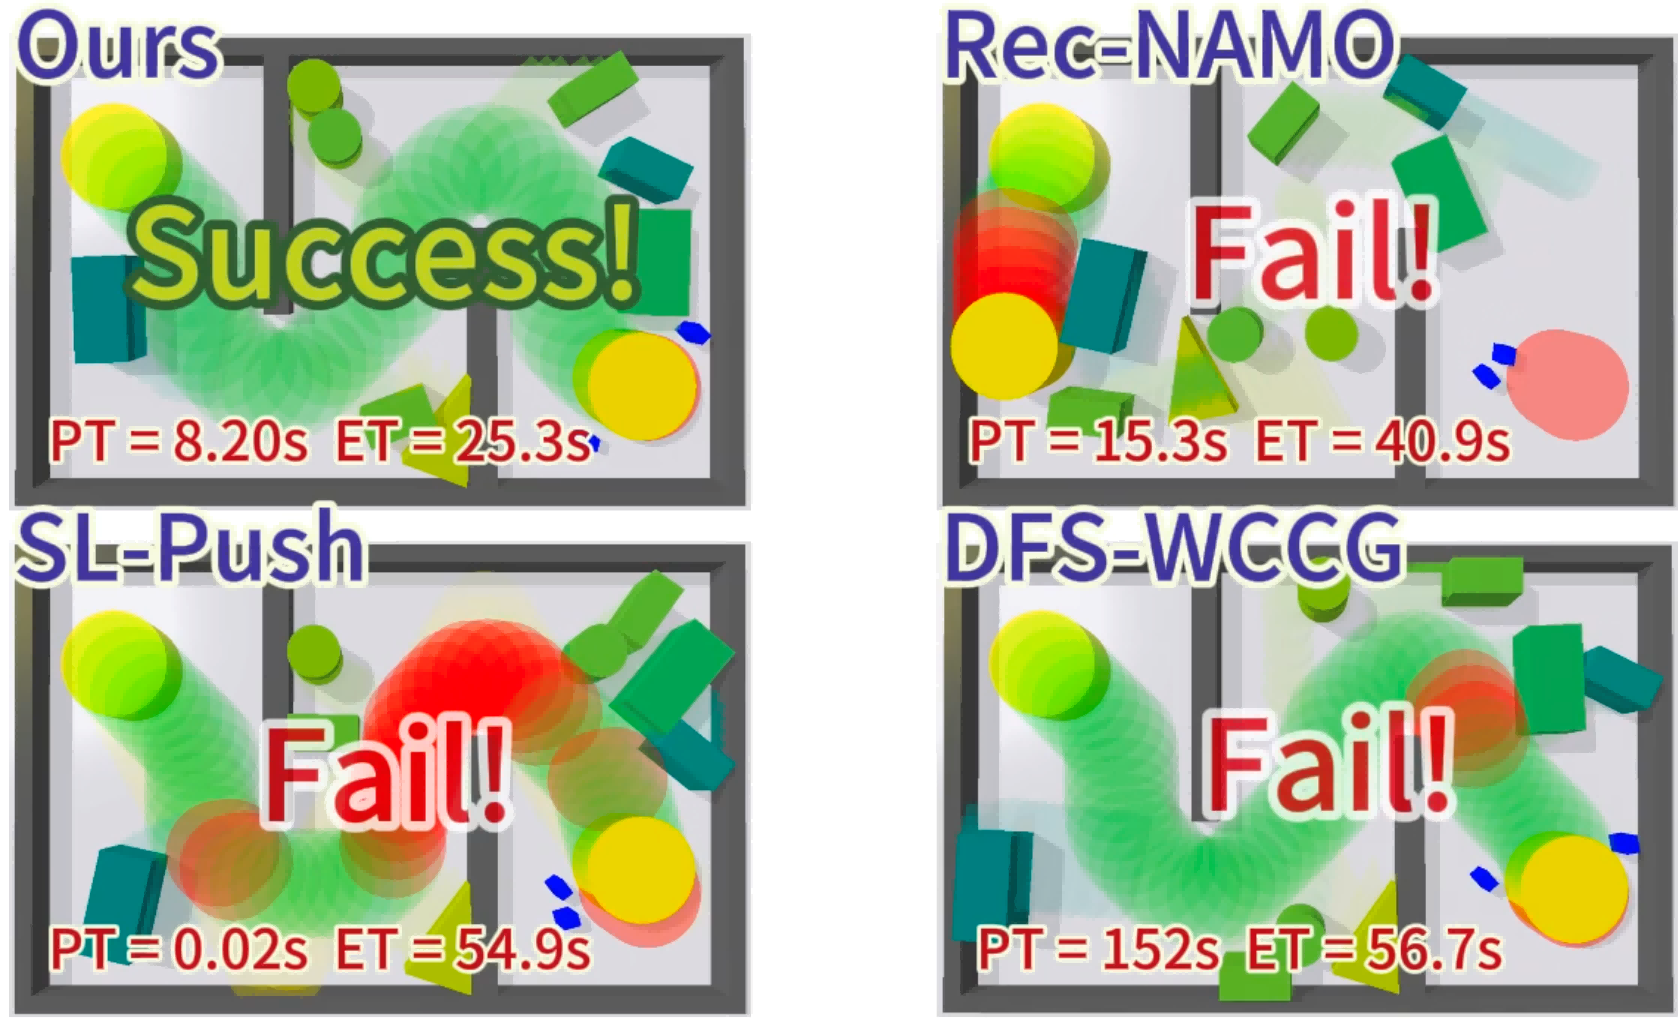
\includegraphics[width=0.7\columnwidth]{figures/compare.png}
 \vspace{-3.0mm}
 \caption{Failure cases by baselines Rec-NAMO, SL-Push and DFS-WCCG.}
 \label{fig:baseline}
 \vspace{-6.0mm}
\end{figure}

% ========================================
%==============================
\subsubsection{Results}
\change{
Across the $40$ Scenario~1 trials, PushAround achieves a $97.5\%$ success rate,
with mean planning and execution times of $10.3$\,s and $28.6$\,s, respectively,
and $6.0$ pushes per successful trial, as shown in Table~\ref{tab:main_ablation}.
Fig.~\ref{fig:main_result} shows representative runs in both scenarios.
In Scenario~1 with $10$ movable obstacles and two robots, PushAround generates
a $6$-push plan in $7.4$\,s and completes execution in $42.3$\,s. In
Scenario~2 with $14$ obstacles, it generates a $9$-push plan in $11.2$\,s,
with $61.3$\,s of execution.
Planning effort is dominated by simulation-based validation: a successful
trial uses $121.5$ simulations on average for $6.0$ executed pushes. The
ablations indicate that mode caching, quick-pass, gap lookahead, and reinsertion
mainly affect this validation load rather than plan length. Execution takes
longer because each selected push is physically carried out and observed,
whereas inter-push repositioning is handled by geometric reachability checks.
}

\change{
\subsubsection{WCCG Connectivity Validation}
\label{subsec:wccg-validation}

WCCG is compared against two references on $300$ random scenes (convex,
non-convex and mixed; Table~\ref{tab:wccg-validation}). The continuous reference (CC) resolves collisions geometrically after inflating boundaries by~$W/2$, with no grid discretization~\cite{lozano1983spatial}; the fine-raster reference (FR) discretizes the workspace on a $0.01$\,m occupancy grid. CC and FR disagree in $4$ of $300$ cases, all near narrow contacts and rasterization-related, whereas WCCG matches CC on all $300$ scenes without false positives or negatives. A query costs $1.07$\,ms ($0.67$\,ms query, $0.40$\,ms construction)
against $1.36$\,ms (CC) and $243$\,ms (FR). It also supplies the gap graph for PIHS. Rebuilt after every simulated or executed push, it is negligible next to the physics rollouts.
}




\subsubsection{Comparisons}\label{subsec:comparisons}
Four baseline variants run on Scenario~1 over $40$ randomized trials under the same $W$-clearance criterion, distribution and simulator:
\textbf{DFS-WCCG} (WCCG-guided search with fixed pushes), \textbf{SL-Push}
(offline and simulation-validated variants), and \textbf{Rec-NAMO} (recursive
NAMO)~\cite{stilman2007manipulation,yao2024local,saxena2023planning,ren2025search}.
Table~\ref{tab:main_ablation} shows that PushAround reaches the highest success
rate, $97.5\%$, at the lowest combined planning-and-execution time among
successful trials ($38.9$\,s).
DFS-WCCG exhibits rapid branching growth, offline SL-Push produces displacements that fail in execution, and Rec-NAMO often fails to connect the $W$-clear corridor in clutter (Fig.~\ref{fig:baseline}).


%==============================
\begin{table}[t]

\caption{\change{Scalability and robustness.}}
\label{tab:generalization}
\vspace{-2.0mm}
\centering
\footnotesize

\renewcommand{\arraystretch}{0.95}
\setlength{\tabcolsep}{3.5pt}

\change{
\begin{tabular}{
 @{}
 l
 c
 c
 r@{\;}c@{\;}l
 @{\hspace{10pt}}
 r@{\;}c@{\;}l
 @{}
}
\hline

Case
& Trials
& Succ.(\%)
& \multicolumn{3}{c@{\hspace{10pt}}}{$PT$ (s)}
& \multicolumn{3}{c}{$ET$ (s)}
\\

\hline

\multicolumn{9}{l}{
 \emph{Obstacle density} (PushAround, $N=2$, nominal)
}
\\

$M=15$
& 10 & 100
& 2.5 & $\pm$ & 0.9
& 37.1 & $\pm$ & 21.0
\\

$M=30$
& 10 & 100
& 11.7 & $\pm$ & 3.7
& 100.9 & $\pm$ & 34.7
\\

$M=45$
& 10 & 100
& 53.4 & $\pm$ & 24.5
& 272.7 & $\pm$ & 97.4
\\

\hline

\multicolumn{9}{l}{
 \emph{Robot-team size} ($M=30$, nominal; 10 trials per cell)
}
\\

PushAround, $N=3$
& 10 & 100
& 30.0 & $\pm$ & 12.7
& 97.3 & $\pm$ & 42.1
\\

PushAround, $N=4$
& 10 & 100
& 29.2 & $\pm$ & 8.9
& 110.1 & $\pm$ & 33.1
\\

SL-Push (sim), $N=3$
& 10 & 80
& 30.0 & $\pm$ & 46.3
& 193.3 & $\pm$ & 111.3
\\

SL-Push (sim), $N=4$
& 10 & 80
& 23.4 & $\pm$ & 18.2
& 171.7 & $\pm$ & 61.2
\\

DFS-WCCG, $N=3$
& 10 & 100
& 142.6 & $\pm$ & 183.1
& 178.1 & $\pm$ & 72.1
\\

DFS-WCCG, $N=4$
& 10 & 90
& 101.9 & $\pm$ & 103.9
& 175.9 & $\pm$ & 113.6
\\

\hline

\multicolumn{9}{l}{
 \emph{Physics mismatch} ($M=30$, $N=2$)
}
\\

Nominal
& 10 & 100
& 16.8 & $\pm$ & 3.4
& 104.7 & $\pm$ & 37.4
\\

Mass $\times 0.6$--$1.4$
& 40 & 100
& 16.8 & $\pm$ & 5.4
& 105.9 & $\pm$ & 44.6
\\

Lateral fric. $\times 0.6$--$1.4$
& 40 & 97.5
& 16.5 & $\pm$ & 5.7
& 114.0 & $\pm$ & 48.5
\\

Spin fric. $\times 0.6$--$1.4$
& 40 & 97.5
& 15.2 & $\pm$ & 3.6
& 100.1 & $\pm$ & 35.7
\\

Force limit $\times 0.6$--$1.4$
& 40 & 95.0
& 18.9 & $\pm$ & 10.9
& 115.9 & $\pm$ & 58.5
\\

All perturbed
& 160 & 97.5
& 16.9 & $\pm$ & 7.0
& 108.9 & $\pm$ & 47.4
\\

\hline

\end{tabular}
}

\vspace{0.5mm}

\begin{flushleft}
\footnotesize
\change{
Each perturbed row scales one parameter; the others stay nominal. Times and budget
are as in Table~\ref{tab:main_ablation}.
}
\end{flushleft}

\vspace{-6.0mm}

\end{table}

%==============================

%==============================
\subsubsection{Ablation Studies}
Four internal ablations are conducted: \textbf{w/o gap-lookahead} (gaps ranked
without downstream costs), \textbf{w/o mode-cache} (no warm start from validated
modes), \textbf{w/o quick-pass} (all candidates evaluated by rollout), and
\textbf{w/o reinsertion} (failed nodes not reconsidered).
Table~\ref{tab:main_ablation} shows that gap-lookahead and reinsertion mainly
improve robustness (success drops by more than $10\%$ when either is removed),
whereas quick-pass also lowers success to $90.0\%$ and mode-cache mainly changes
the simulation count.


\change{

\subsubsection{Scalability and Robustness Analysis}
\label{subsec:generalization}

Generalization studies use an $8\times8$\,m workspace
(Table~\ref{tab:generalization}, Figs.~\ref{fig:scalability_scenes}--\ref{fig:density_scaling}).
\minorchange{Density runs query a precomputed mode table (preparation excluded from $PT$);
mismatch and team-size runs optimize modes greedily. At $M{=}30$, $N{=}2$,
nominal $PT$ is $11.7$, $16.8$ and $23.9$\,s, respectively; the team-size
study uses a different scene realization of the same seeds.}
\textbf{(I) Obstacle density:} with two robots, $10$ trials per density,
PushAround keeps $100\%$ success at all tested densities ($M{=}15$ to $45$), planning in $2.5$--$53.4$\,s; at $M{=}45$ none of the evaluated baselines solves any trial
and the no-recursion ablation solves $7/10$.
\textbf{(II) Robot-team size:} at $M{=}30$, PushAround solves all ten trials at
$N{=}2$, $3$, and $4$ using the same mode-generation
procedure with a full-team-first fallback that may leave one robot temporarily inactive.
Across the clutter sweep, branching stays near six while expansions rise
from $3.5$ to $24.5$. A solved trial needs a median of $10$ expansions and
$48$ visited snapshots and about $60$ simulations at $165$\,ms each,
against $22$\,ms per generated mode. Across $N{=}2$--$4$, search effort remains similar
($10$ expansions, $60$--$63$ simulations), while aggregate mode-generation
time rises from $15.8$ to $46.4$\,s.
\textbf{(III) Physics mismatch:} the planner keeps the nominal model and only
the execution simulator is perturbed, one parameter at a time.
PushAround solves $156/160$ perturbed trials ($97.5\%$); under $\pm40\%$
perturbations SL-Push (sim) solves $13/40$ and DFS-WCCG $23/40$.
Averaging successful-trial $PT$ over conditions with successes gives $31.5$
and $229.1$\,s, versus $18.4$\,s for PushAround.
\minorchange{These paired, single-parameter trials reuse ten base seeds (five for
baselines), whose nominal success is $3/5$ versus $10/10$ for PushAround.
Comparisons reflect end-to-end performance rather than normalized
degradation; joint parameter errors are untested.}

}



% ========================================
\begin{figure}[t!]
 \centering
 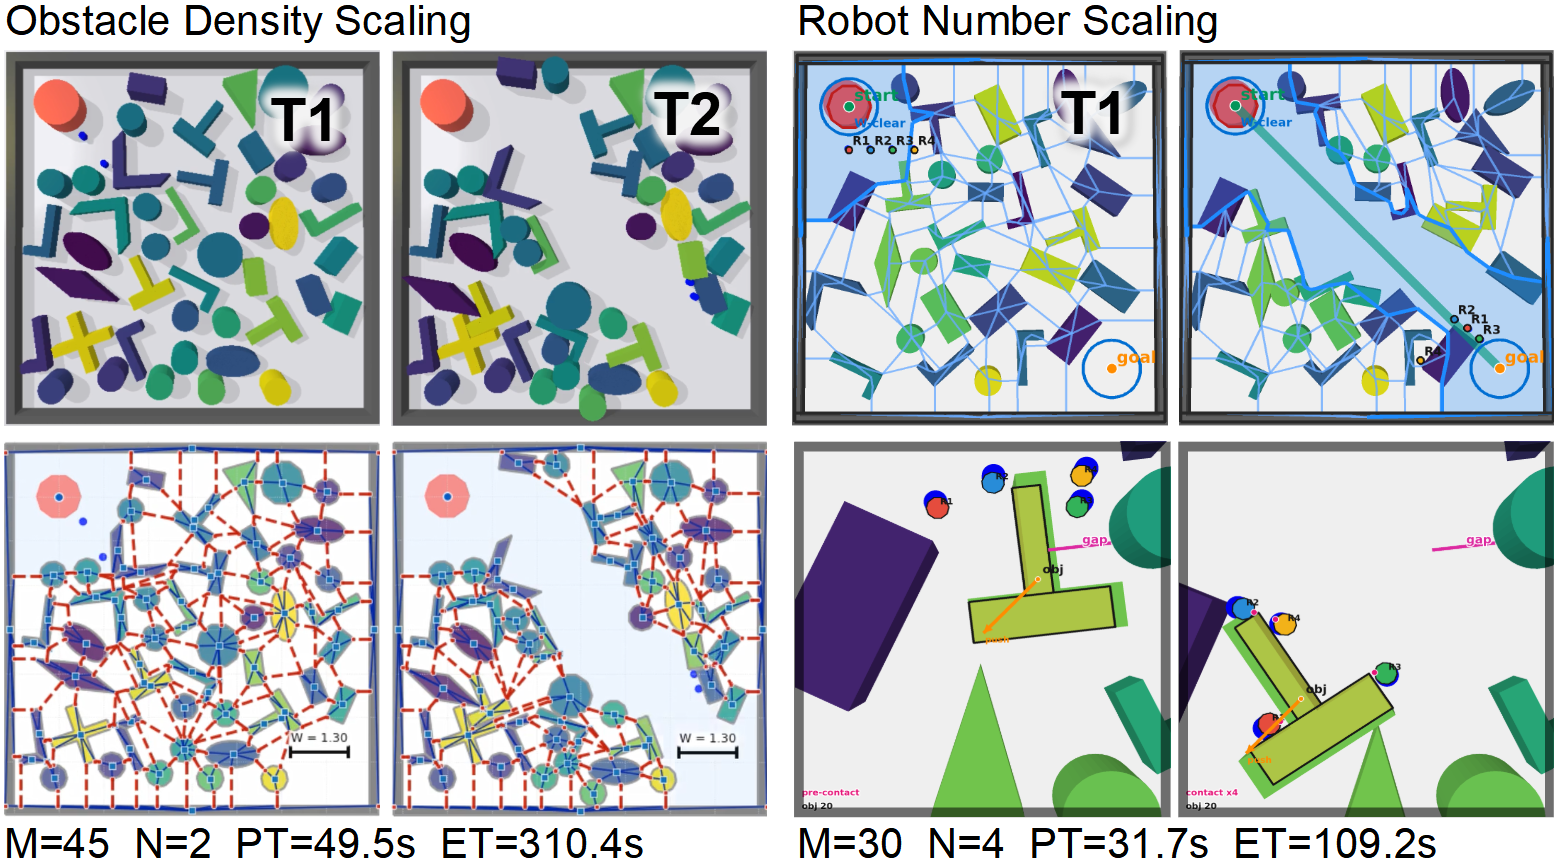
\includegraphics[width=0.9\columnwidth]{figures/obs_rob_scale.png}
 \vspace{-2mm}
 \caption{\change{
 Scalability of the clearing process. \textbf{Left:} density scaling ($M{=}45$, two robots): snapshots during clearing (\textbf{top}) and WCCG overlays with the start face in blue (\textbf{bottom}). \textbf{Right:} team scaling ($M{=}30$, four robots): initial and final states (\textbf{top}) and one push before contact and during execution (\textbf{bottom}).}}
 \label{fig:scalability_scenes}
 \vspace{-3mm}
\end{figure}

% ========================================
% ========================================
\begin{figure}[t!]
 \centering
 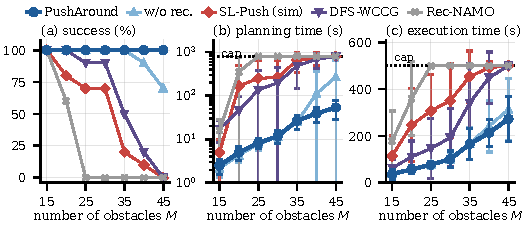
\includegraphics[width=0.95\columnwidth]{figures/density_comparison.pdf}
 \vspace{-2.0mm}
 \caption{\change{
 Obstacle-density scaling ($8\times 8$\,m, $10$ seeds per density). Times are
 budget-capped (planning $800$\,s, execution $20{,}000$ steps $=500$\,s; dotted).}}
 \label{fig:density_scaling}
 \vspace{-4.0mm}
\end{figure}

% ========================================
% ========================================
% ========================================
\begin{figure*}[!t]
 \centering
 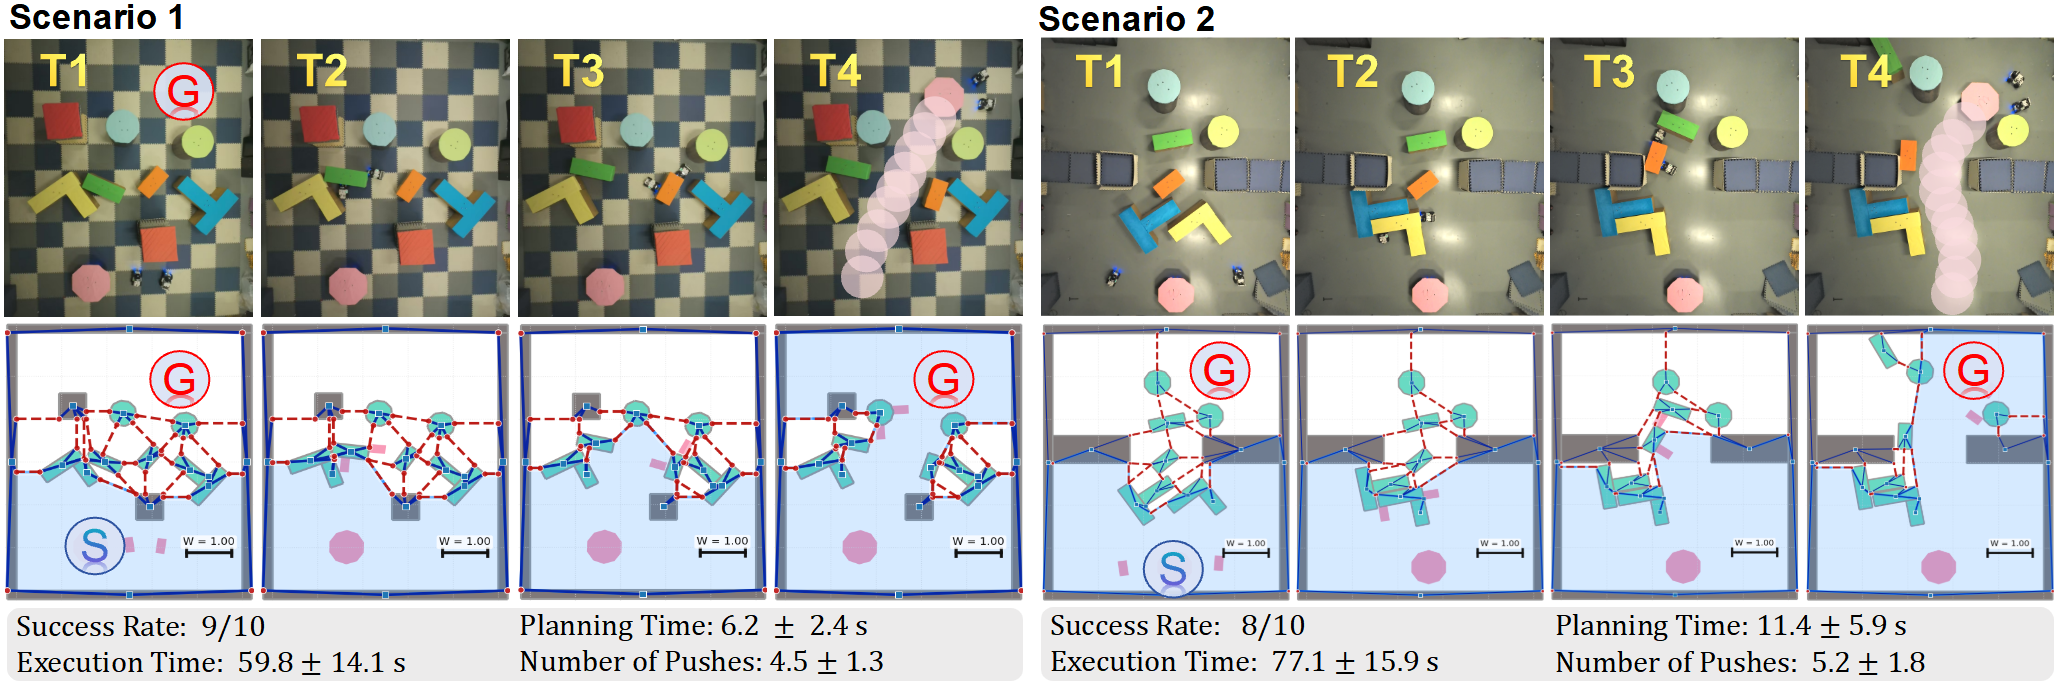
\includegraphics[width=0.95\linewidth]{figures/hardware.png}
 \vspace{-2.0mm}
 \caption{\change{Real-world pushing experiments with execution--planning alignment (over~$20$ runs, $2$ scenarios).
 \textbf{Top:} two robots pushing obstacles in a \(5{\times}6\,\mathrm{m}\)
 workspace. \textbf{Bottom:} WCCG overlays with the start face in blue.}}
 \vspace{-5.0mm}
 \label{fig:hardware}
\end{figure*}

\subsection{Hardware Experiments}\label{subsec:hardware}

\subsubsection{System Description}\label{subsec:exp-description}
Experiments use a $5\times6$\,m workspace of interlocking $0.6\times0.6$\,m foam mats (Fig.~\ref{fig:hardware}), $2$ UGVs and $6$ cardboard boxes; robots and movables carry motion-capture markers streamed to \texttt{PyBullet} in real time.
\change{The UGVs are velocity-controlled, and the optimized contact forces are used only for feasibility evaluation, not for motor control.
\minorchange{Motion-capture poses are compared with $\mathsf{EvalSim}$ predictions:
position or orientation errors above $0.3$\,m or $\pi/4$ trigger replanning,
as do the failures in Sec.~\ref{subsec:execute}.}}

\subsubsection{Results}\label{subsec:exp-results}
Two representative real-world runs are shown in Fig.~\ref{fig:hardware}.
In hardware Scenario~1, PIHS considers five candidate gaps and plans a four-task schedule in $6.5$\,s ($12$ node expansions, $49$ visited snapshots, search depth $6$); the robots then execute it, first rotating the yellow L-shaped object to open a gap near an
immovable obstacle and then separating the green and orange objects until a $W$--clear path is established at $t=52\,$s.
In hardware Scenario~2, PushAround succeeds in $8/10$ trials with an average of $5.2$
pushes and $11.4$\,s of planning; the first direct push on the blue L-shaped
object also moves the adjacent T-shaped block and opens the first gap.
\change{This neighboring-object motion is not a separately encoded action but
an emergent outcome of the coupled rigid-body rollout in $\mathsf{EvalSim}$,
whose snapshot updates the WCCG and execution continues.}
\change{\minorchange{Execution takes $77.1\pm15.9$\,s (mean $\pm$ standard deviation);}
online replanning compensates for deviations due to force limits,
drifting and wheel slippage.}

%%========================================
\section{Conclusion} \label{sec:conclusion}
\change{This work presents PushAround, a multi-robot framework that jointly plans
obstacle selection, contact points and pushing forces through a hybrid search,
and demonstrates hardware feasibility with state-feedback replanning. Future work
targets obstacle-state estimation without external sensing, uncertain masses and
limited robot visibility.}

%%========================================


%========================================
\bibliographystyle{IEEEtran}
\bibliography{contents/references}

\end{document}
"
\ifdefined\CLEANCOPY
  \renewcommand{\minorchange}[1]{#1}
\fi

%%%%%%%%%%%%%%%%%%%%%%%%%%%%%%%%%%%%%%%%%%%%%%%%%%%%%%%
%%%%


% Publication metadata for RA-L 26-3602.
% Author spellings, order, keywords and received date follow PaperCept.
% Revised and accepted dates confirmed by the author on October 20, 2026.
\newcommand{\RALReceivedDate}{June 24, 2026}
\newcommand{\RALRevisedDate}{September 16, 2026}
\newcommand{\RALAcceptedDate}{October 20, 2026}
% RA-L specifies the month/year of final submission in the preprint header.
\newcommand{\RALFinalMonthYear}{October, 2026}

\title{PushAround: Collaborative Path Clearing via Physics-Informed Hybrid Search}

\author{Zili Tang$^{1}$, Zongyuan Li$^{2}$, Zishao Qiao$^{1}$, and Meng Guo$^{1}$%
\thanks{Manuscript received: \RALReceivedDate; Revised: \RALRevisedDate;
Accepted: \RALAcceptedDate.}%
\thanks{This paper was recommended for publication by Editor M. Ani Hsieh
upon evaluation of the Associate Editor and Reviewers' comments.
This work was supported by the National Natural Science Foundation of China
under grants U2241214 and T2121002.
\textit{(Corresponding author: Meng Guo.)}}%
\thanks{The authors are with Peking University, Beijing 100871, China:
$^{1}$School of Advanced Manufacturing and Robotics;
$^{2}$College of Engineering (e-mail: meng.guo@pku.edu.cn).}%
\thanks{Digital Object Identifier (DOI): see top of this page.}}

\markboth{IEEE Robotics and Automation Letters. Preprint Version. Accepted \RALFinalMonthYear}%
{Tang \MakeLowercase{\textit{et al.}}: PushAround: Collaborative Path Clearing}


% --- float packing (revision) ---
\setcounter{topnumber}{3}
\setcounter{dbltopnumber}{3}
\renewcommand{\topfraction}{0.92}
\renewcommand{\dbltopfraction}{0.92}
\renewcommand{\textfraction}{0.07}
\renewcommand{\floatpagefraction}{0.75}

\begin{document}
\maketitle


%%========================================


%%========================================
\begin{abstract}
Large vehicles in cluttered environments are often blocked by movable
obstacles, motivating mobile robot teams to clear traversable corridors.
Navigation Among Movable Obstacles (NAMO) approaches often abstract obstacle
displacements while neglecting robot dimensions, obstacle mass, contact
geometry and forces, yielding physically infeasible plans.
\emph{PushAround} is a physics-informed hybrid search that couples geometric
connectivity reasoning with short-horizon simulation to construct executable
clearing plans. Repeated W--clearance connectivity graph (WCCG) queries expose
frontier gaps requiring widening and rank them by estimated downstream costs.
The search generates direct or recursive pushing candidates, selecting
obstacles, directions, contacts and forces, and admits physics-validated
candidates.
\change{
Numerical experiments validate WCCG against standard connectivity checks and
demonstrate scaling to denser clutter and teams of up to four robots, with
robustness to simulated execution-side physical-parameter mismatch.
}
\end{abstract}

\begin{IEEEkeywords}
Multi-Robot Systems, Task and Motion Planning, Manipulation Planning.
\end{IEEEkeywords}
%%========================================
\section{Introduction}\label{sec:intro}
\IEEEPARstart{I}{n} warehouses, disaster sites and urban spaces, movable
obstacles such as pallets, boxes and equipment can block large vehicles,
motivating mobile robot teams to clear traversable corridors.
Conventional path planners assume static obstacles and fail once routes are
blocked~\cite{liu2023path}. Navigation Among Movable Obstacles (NAMO) creates
routes by pushing, pulling or rotating obstacles~\cite{stilman2005navigation},
yet many methods abstract away robot dimensions, obstacle size and mass,
contact geometry, forces and dynamics, producing \emph{geometrically valid
but physically unrealizable plans}. As shown in Fig.~\ref{fig:snapshots},
a large robot may be unable to reach obstacle boundaries while a small
robot lacks pushing force. Cooperative pushing by several small robots
offers an alternative, but simultaneous pushes can trigger chained motions
of several obstacles, introducing physical coupling that complicates planning.

%==============================================
\begin{figure}[t!]
  \centering
  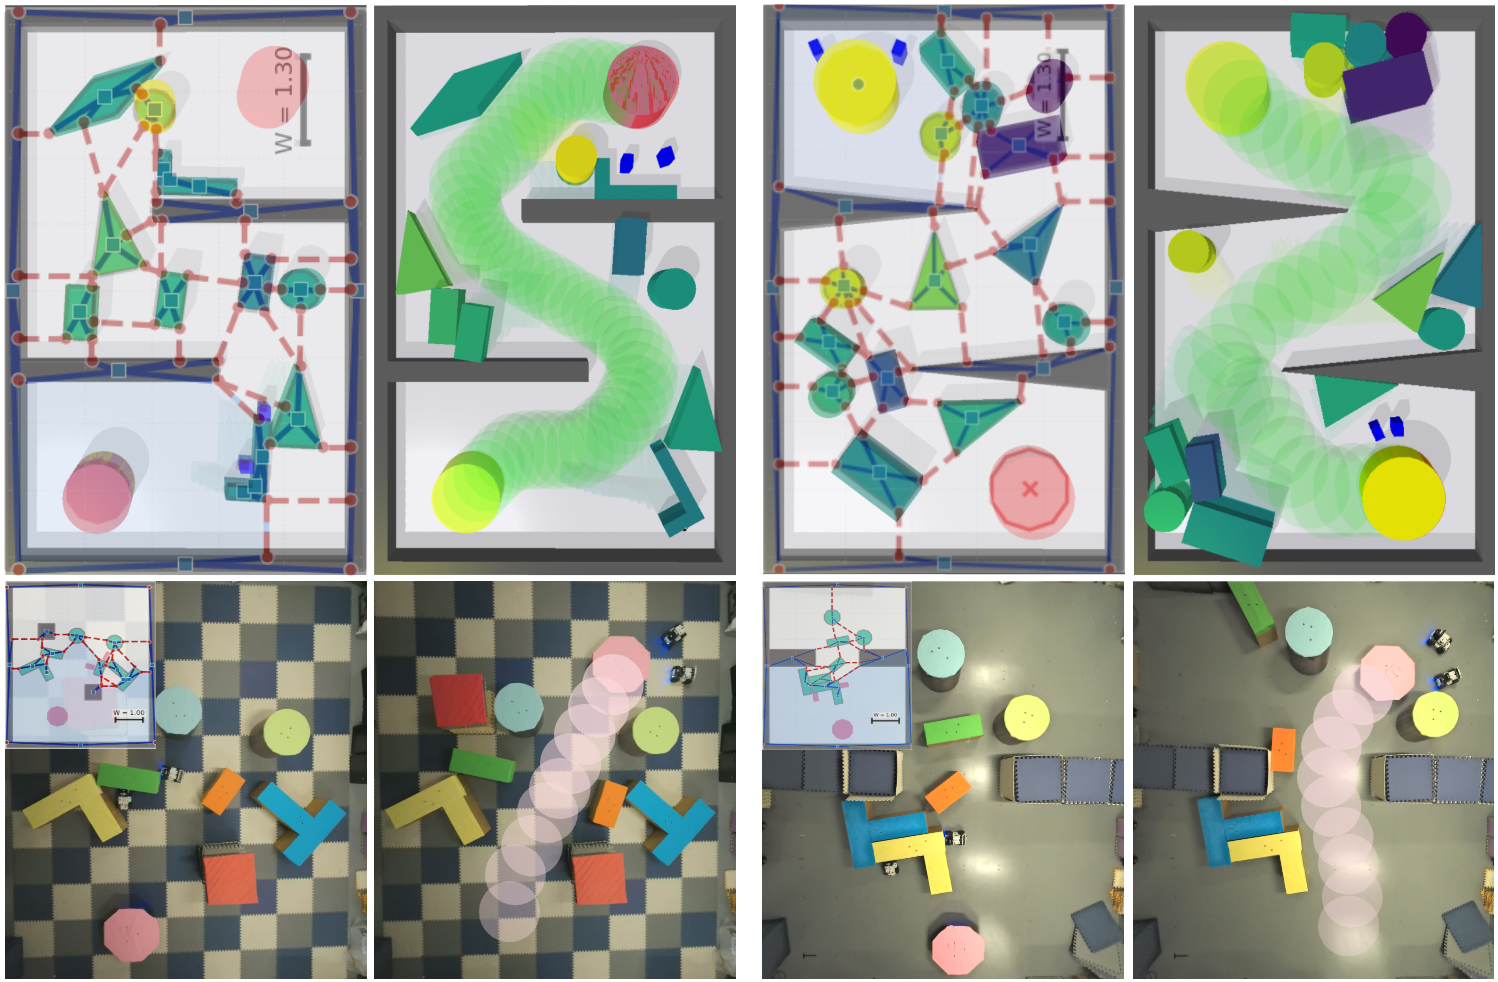
\includegraphics[width=0.9\linewidth]{figures/cover.png}% or {presearch.pdf}
  \vspace{-0.1in}
  \caption{
    Collaborative path clearing in simulation (\textbf{Top})
    and hardware (\textbf{Bottom}). Two robots push movable obstacles to
    create a $W$--clear path for a large vehicle from start to goal.
  }
  \vspace{-6mm}
  \label{fig:snapshots}
\end{figure}

%==============================================

\subsection{Related Work}\label{subsec:intro-related}

\looseness=-1
NAMO extends motion planning to cluttered environments by planning obstacle
displacements through pushing, pulling, or
rotating~\cite{stilman2005navigation,stilman2007manipulation}. Later work considers heuristic search, learning-based local planning, physics-based rollouts, and collaborative pushing~\cite{stilman2007manipulation,yao2024local,ren2025search,weeda2025pushing,tang2026pushingbots}.



%==============================================
\begin{figure*}[t!]
  \centering
  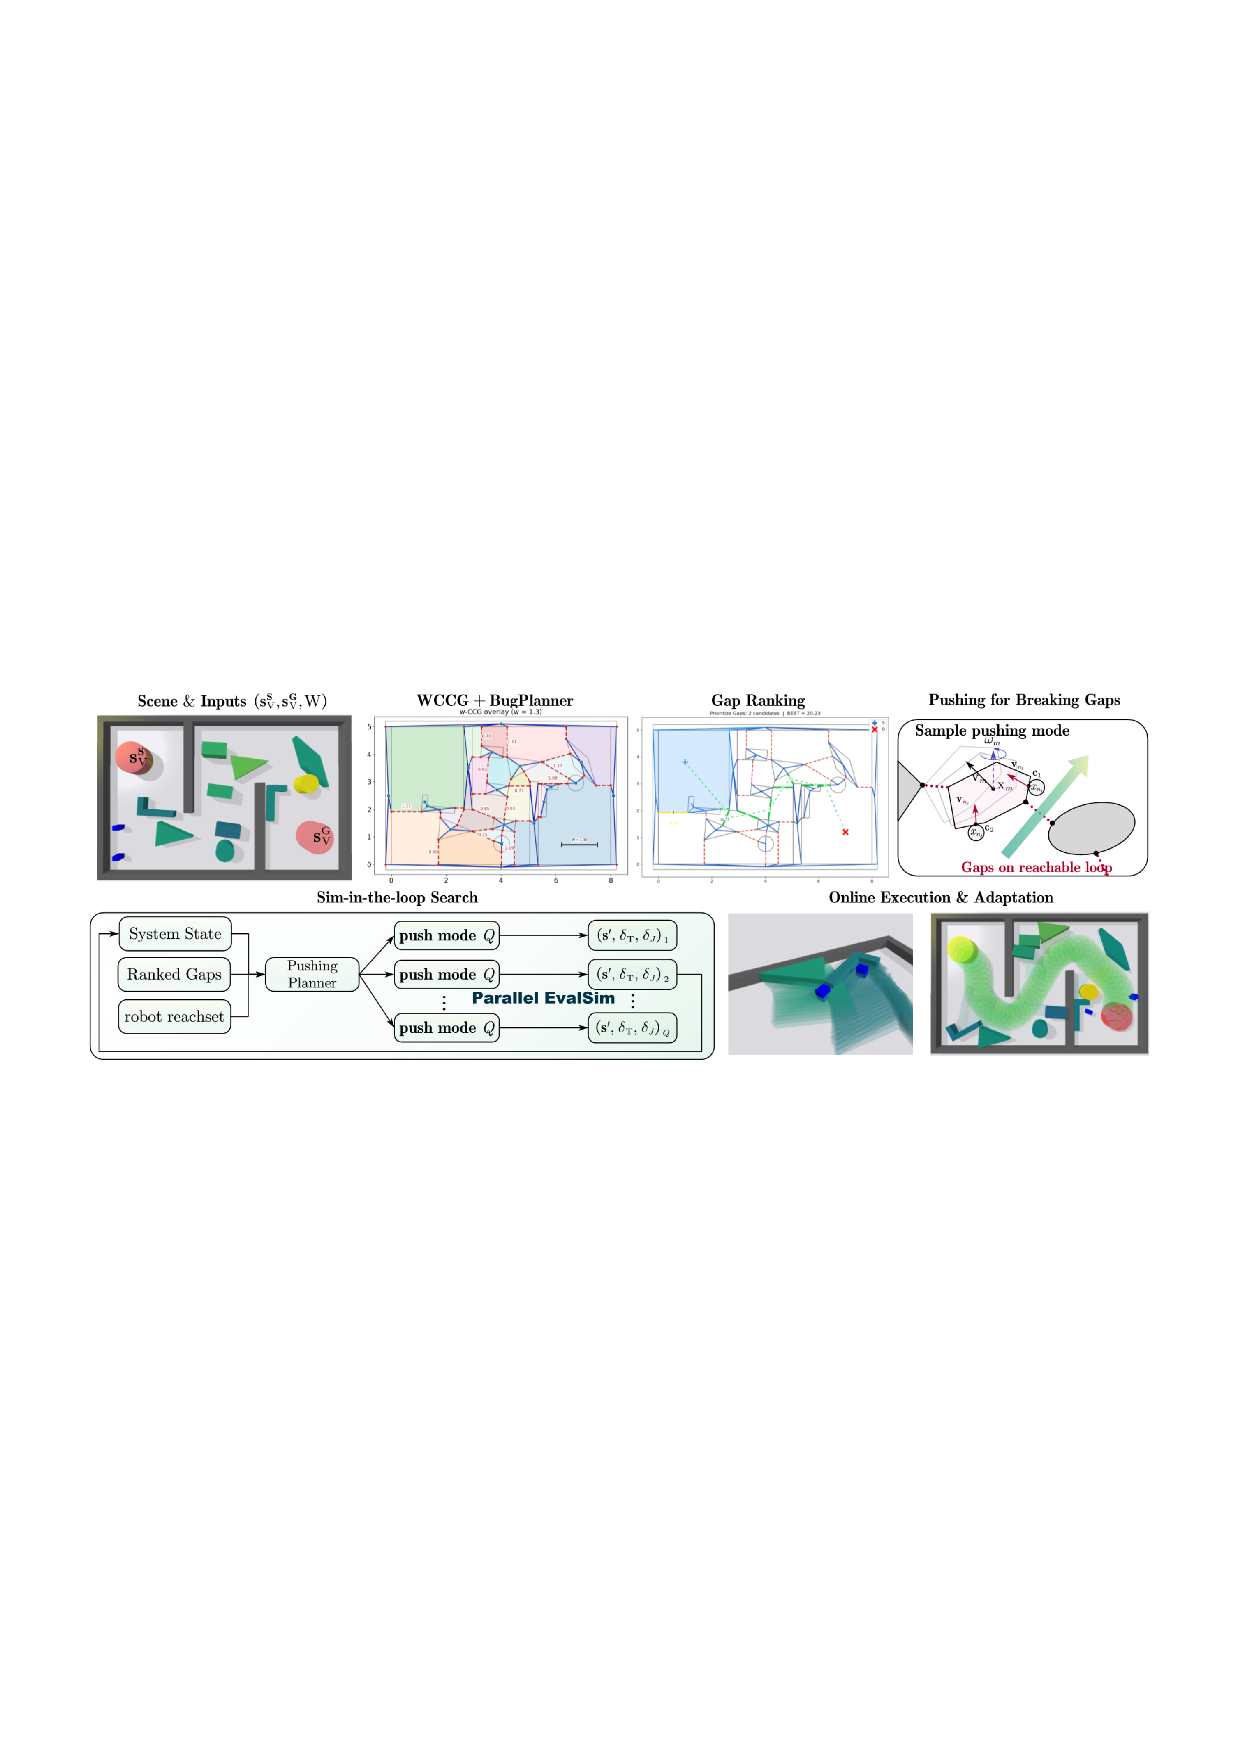
\includegraphics[width=0.84\linewidth]{figures/overall.pdf}
  \vspace{-0.1in}
\caption{Overview of the proposed framework.
\textbf{Top:} Scene inputs, WCCG construction, gap ranking, and sampling of pushing
modes for breaking frontier gaps;
\textbf{Bottom-left:} Sim-in-the-loop hybrid search with parallel validation in simulation;
\textbf{Bottom-right:} Online execution and adaptation during path clearing.}
  \label{fig:overall}
  \vspace{-5mm}
\end{figure*}
%==============================================


Collaborative pushing has been widely studied in multi-robot manipulation:
foundational work on the mechanics of pushing and limit surfaces~\cite{goyal1989limit,lynch1992manipulation}, cooperative transport with robot swarms~\cite{chen2015occlusion}, multi-robot box pushing with reinforcement learning~\cite{wang2006multi}, collaborative pushing of polytopic objects in cluttered scenes~\cite{tang2026pushingbots}, and learning-based loco-manipulation~\cite{feng2025learning}. These studies focus on a prescribed object rather than multi-object corridor clearing.

Physics-informed planning incorporates dynamics models, contact reasoning, or
simulation feedback into motion generation: learned dynamics for humanoid
contact planning~\cite{lin2019efficient}, multi-contact force control~\cite{rouxel2024multi}, demonstration-guided optimal control over contact modes~\cite{xue2023demonstration}, physics simulation interleaved with multi-agent pathfinding~\cite{saxena2023planning,ren2025object}, and learned physical priors~\cite{ni2023progressive,liu2025physics}. \change{These methods consider a prescribed target or few objects, whereas corridor clearing requires rearranging many obstacles to admit a larger vehicle.}


%==============================
\subsection{Our Method}\label{subsec:intro-our}

As shown in Fig.~\ref{fig:overall}, this work introduces \textbf{PushAround},
a physics-informed framework for collaborative multi-robot pushing that
constructs traversable corridors for large vehicles in cluttered environments.
Its central novelty is a hybrid search that jointly determines which obstacles
to displace and how to push them, coupling the high-level clearing sequence
with low-level pushing modes specifying contact points, directions and forces.
The framework integrates a W--clearance connectivity graph (WCCG) that certifies
vehicle passage under width constraints, frontier-gap ranking by estimated
effort, and pushing-mode generation under geometric and actuation constraints.
Guided by the selected gap, the search proposes direct pushes or recursively
clears blocking obstacles, and expands the plan through physics-validated
transitions that account for robot dimensions, object mass, contact geometry
and coupled pushing dynamics. Execution feedback updates connectivity and
triggers replanning when needed.
% \change{We further examine its robustness to physical-model uncertainty relevant to real-world deployment.}



The contributions are twofold: {(I)} it introduces a unified framework that
couples collaborative pushing with physics-informed verification, 
producing executable plans for path clearing in cluttered environments; 
and {(II)} \change{ 
it demonstrates empirical gains in feasibility, efficiency and scalability over evaluated NAMO and
collaborative-clearing baselines, with robustness to execution-side physics
mismatch.
}

%%========================================
\section{Problem Description}\label{sec:problem}
%==============================
\subsection{Workspace and Robots}\label{subsec:ws}
The workspace is a bounded planar region $\mathcal{W}\subset\mathbb{R}^2$
containing immovable structures~$\mathcal{O}\subset\mathcal{W}$ and $M\geq0$
movable rigid polygons
$\boldsymbol{\Omega}\triangleq\{\Omega_1,\cdots,\Omega_M\}\subset\mathcal{W}$.
Each movable obstacle~$\Omega_m$ has mass~$\mathsf{M}_m$,
inertia~$\mathsf{I}_m$, frictional parameters and state
$\mathbf{s}_m(t)\triangleq(\mathbf{x}_m(t),\psi_m(t))$, with
$\mathbf{x}_m(t)\in\mathbb{R}^2$ the centroid position and
$\psi_m(t)\in\mathbb{R}$ the orientation; $\Omega_m(t)$ denotes the region it
occupies at time~$t$. A team of~$N$ robots,
$\mathcal{R}\triangleq\{R_1,\cdots,R_N\}$, operates as a cooperative unit. Each
robot~$R_i$ is a rigid body with state
$\mathbf{s}_{R_i}(t)\triangleq(\mathbf{x}_{R_i}(t),\psi_{R_i}(t))$ and
footprint~$R_i(t)$. The instantaneous free space is given by:
\begin{equation}\label{eq:freespace}
\widehat{\mathcal{W}}(t)\triangleq\mathcal{W}\setminus\Big(
\mathcal{O}\cup\{\Omega_m(t)\}_{m=1}^{M}\cup\{R_i(t)\}_{i=1}^{N}
\Big),
\end{equation}
where~$\widehat{\mathcal{W}}(t)$ excludes regions occupied by immovable
obstacles, movable obstacles, and robots.

%==============================
\subsection{External Vehicle and Clearance Goal}\label{subsec:vehicle}
An external vehicle~$\texttt{V}$ whose footprint is enclosed by a disk of
radius~$W/2>0$ must navigate within the workspace from a start position
$\mathbf{x}_\texttt{V}^{\texttt{S}}\in\mathcal{W}$ to a goal position
$\mathbf{x}_\texttt{V}^{\texttt{G}}\in\mathcal{W}$. Since movable obstacles may
obstruct the way, the clearance goal is to rearrange them so that the workspace
contains a passage from~$\mathbf{x}_\texttt{V}^{\texttt{S}}$ to
$\mathbf{x}_\texttt{V}^{\texttt{G}}$ that can accommodate this enclosing disk,
i.e., a passage of width at least~$W$. At time~$t$, this is expressed by the
admissible reference-center space
$\mathcal{F}_W(t)\triangleq
\{p\in\widehat{\mathcal{W}}(t)\mid
\mathbb{B}_{W/2}(p)\subset\widehat{\mathcal{W}}(t)\}$, where
$\mathbb{B}_{W/2}(p)$ is the disk of radius~$W/2$ centered at~$p$. The
$W$-clearance condition is then given by:
\begin{equation}\label{eq:wclear}
\exists\,\mathcal{P}^W_\texttt{V}\subset\mathcal{F}_W(t):\
\mathbf{x}_\texttt{V}^{\texttt{S}}\leadsto\mathbf{x}_\texttt{V}^{\texttt{G}},
\end{equation}
which certifies a collision-free centerline path for any vehicle footprint
contained in the enclosing disk.
% Since movable obstacles may obstruct the way,
% a direct passage is not always feasible.
% At time~$t$, the admissible center positions of~$\texttt{V}$ are
% \begin{equation}
% \mathcal{F}_W(t)\triangleq
% \{p\in\widehat{\mathcal{W}}(t)\mid \mathbb{B}_{W/2}(p)\subset\widehat{\mathcal{W}}(t)\}.
% \end{equation}
% where $\mathbb{B}_{W/2}$ is a disk of radius~$W/2$.
% The clearance goal is satisfied if there exists a continuous centerline path
% inside~$\mathcal{F}_W(t)$:
% \begin{equation}\label{eq}
% \exists\,\mathcal{P}^W_\texttt{V}\subset\mathcal{F}_W(t):
% \mathbf{x}_\texttt{V}^{\texttt{S}}\leadsto\mathbf{x}_\texttt{V}^{\texttt{G}}.
% \end{equation}
% this therefore certifies a passage with width at
% least~$W$.


%==============================


\subsection{Collaborative Pushing Modes}\label{ss:interaction_mode}
To enlarge blocked gaps, the robots may actively
reconfigure~$\boldsymbol{\Omega}$ by pushing movable obstacles. For obstacle
$\Omega_m\in\boldsymbol{\Omega}$, a pushing mode is denoted by
$\boldsymbol{\xi}_m\triangleq(\mathbf{c}_m,\mathbf{u}_m)$, where
$\mathbf{c}_m=(c_1,\cdots,c_N)$ is an ordered tuple of contact points on
$\partial\Omega_m$, and the ordering specifies the robot-to-contact assignment.
The vector~$\mathbf{u}_m\in\mathbb{R}^{2N}$ stacks the corresponding planar
contact forces, expressed in the body frame of~$\Omega_m$; \change{an inactive
robot carries a null contact $c_i=\varnothing$ with zero force.}
For a contact tuple~$\mathbf{c}_m$, the set of admissible forces
${U}_m(\mathbf{c}_m)\subset\mathbb{R}^{2N}$ collects contact forces
satisfying the robot pushing limits, robot--object friction, and unilateral
contact constraints. The body wrench induced by a mode is defined as:
\begin{equation}
\mathbf{q}_m(\boldsymbol{\xi}_m)
\triangleq
G_m(\mathbf{c}_m)\mathbf{u}_m,
\label{eq:contact_wrench_map}
\end{equation}
where~$G_m(\mathbf{c}_m)\in\mathbb{R}^{3\times 2N}$ is the contact-to-wrench mapping;
and $\mathbf{q}_m(\boldsymbol{\xi}_m)\in\mathbb{R}^3$.
The admissible mode set is state dependent as denoted by~$\Xi_m(\mathbf{s})$.
It contains modes whose contacts are reachable from the
current robot configurations, pre-contact configurations are feasible in
the current clutter, and forces satisfy
$\mathbf{u}_m\in{U}_m(\mathbf{c}_m)$. Hence, applying a feasible
mode~$\boldsymbol{\xi}_m\in\Xi_m(\mathbf{s}(t))$ yields the physical
transition:
\begin{equation}\label{eq:transition}
  \mathbf{s}(t^+)\triangleq
  \Phi\big(\mathbf{s}(t),\,m,\,\boldsymbol{\xi}_m\big),
\end{equation}
where~$\mathbf{s}(t)$ stacks all robot and obstacle states.
\change{
The force vector~$\mathbf{u}_m$ serves as a feasibility variable to certify
wrench generation under the modeled contact and actuation constraints rather
than a directly commanded control input.
}


%==============================
\subsection{Problem Statement}\label{subsec:objective}

The goal is to compute a \emph{hybrid schedule} that reconfigures movable
obstacles to admit a $W$-feasible path for the external vehicle.
The schedule is defined as:
\begin{equation}\label{eq:schedule}
    \pi\triangleq
    \left\{
    \left(
    \Omega_{m_k},
    \mathbf{v}_k,
    \boldsymbol{\xi}_k
    \right)
    \right\}_{k=1}^{K},
\end{equation}
where~$\Omega_{m_k}\in\boldsymbol{\Omega}$ is the manipulated obstacle,
$\mathbf{v}_k$ its pushing direction, $\boldsymbol{\xi}_k\in\Xi_{m_k}$ its
pushing mode. The node cost is:
\begin{equation}\label{eq:problem}
    \mathcal{J}_{\mathrm{clr}}(\pi)
    \triangleq
    T+
    \alpha
    \sum_{k=1}^{K}
    J\left(
    m_k,\boldsymbol{\xi}_k,\mathbf{s}(t_k)
    \right),
\end{equation}
\change{where~$T\triangleq\sum_{k=1}^{K}\Delta t_k$ denotes 
the robotic clearance duration excluding vehicle traversal,  
with $\Delta t_k>0$ the duration that the evaluation in~(13) returns for the $k$-th push,
 and~$J(\cdot)$ is the simulation-estimated manipulation cost. 
 Vehicle traversal enters only through the terminal $W$-clearance condition~\eqref{eq:wclear}. 
 The constraints~\eqref{eq:freespace}--\eqref{eq:transition} 
 enforce valid pushing transitions. 
 Equation~\eqref{eq:problem} defines the realized clearance cost; PIHS samples finitely and does not guarantee optimality.}

% ==============================
\begin{remark}\label{remark:uniqueness}
  \change{The objective couples obstacle selection, pushing-mode generation and switching into one hybrid planning problem, yielding a combinatorial-continuous search space richer than classical NAMO formulations with hand-crafted contact modes~\cite{goyal1989limit,chen2015occlusion,wang2006multi}.}
  \hfill~$\blacksquare$
\end{remark}
% ==============================

%%========================================
% %% ========================================
\section{Proposed Solution}\label{sec:solution}

As shown in Figs.~\ref{fig:overall} and~\ref{fig:pihs_overview}, PushAround first
uses the W-Clearance
Connectivity Graph in Sec.~\ref{subsec:wccg} and gap ranking in
Sec.~\ref{subsec:gap} to identify and prioritize blocking gaps. It then
generates and evaluates physically feasible collaborative pushing modes in
Sec.~\ref{subsec:push}. These components are integrated into the
simulation-in-the-loop hybrid search of Sec.~\ref{subsec:simloop} and the online
execution procedure of Sec.~\ref{subsec:overall}.





% %% ========================================
%==============================================
\subsection{W--Clearance Connectivity Graph}\label{subsec:wccg}

The feasibility of routing the vehicle reduces to whether a~$W$-width corridor
connects~$\mathbf{x}_\texttt{V}^{\texttt{S}}$ and~$\mathbf{x}_\texttt{V}^{\texttt{G}}$.
A W--clearance connectivity graph (WCCG) is introduced here to encode obstacle
adjacencies under clearance~$W$ and enable fast connectivity queries.
\change{Conventional clearance checks either rasterize the workspace into an
inflated occupancy grid or query sampling-based roadmaps, and must therefore fix
a resolution and re-query the map whenever an obstacle
moves~\cite{karaman2011samplingbasedalgorithmsoptimalmotion}.
Built directly from obstacle geometry, the WCCG introduces no grid-resolution parameter in the repeated connectivity queries used during planning.}

%------------------------------
\begin{figure}[t!]
  \centering
  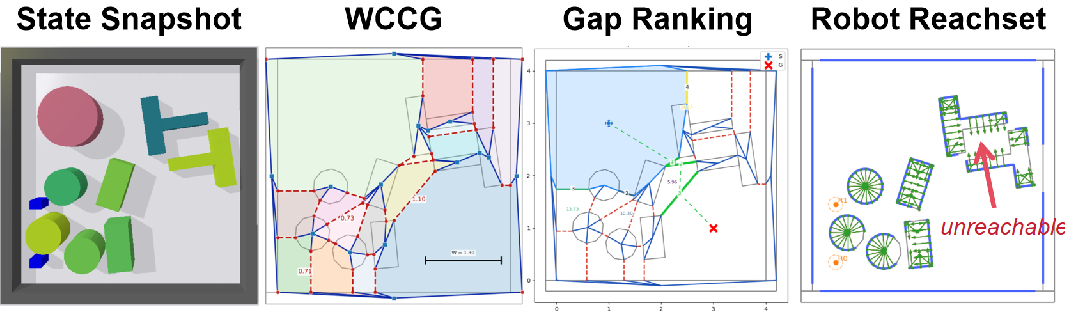
\includegraphics[width=0.9\linewidth]{figures/PIHS_top.pdf}
  \vspace{-2mm}
  \caption{\change{Core components of the physics-informed hybrid search: WCCG
  construction, gap ranking, mode generation, and physics validation.}}
  \label{fig:pihs_overview}
  \vspace{-4mm}
\end{figure}
%------------------------------

\subsubsection{Graph Construction}
The WCCG is built by decomposing all clearance-relevant obstacle and workspace
boundaries into convex components or segments.
From each component~$C$,
a centroid node~$v_c$ is created. When two components~$C_u$ and~$C_v$
have closest points~$p_u\in C_u$ and~$p_v\in C_v$ with distance less than~$W$,
bridge nodes are added at~$p_u$ and~$p_v$. These bridge nodes are
connected by a bridge--bridge edge, annotated with the gap width
$w_{uv}\triangleq\|p_u-p_v\|$, and further linked back to their centroids with
centroid--bridge edges. Narrow passages with~$w_{uv}<W$ are marked
as potential bottlenecks. The resulting graph is given by:
\begin{equation}\label{eq:wccg}
\mathcal{G}_W\triangleq(\mathcal{V},\; \mathcal{E}_c\cup\mathcal{E}_b),
\end{equation}
where~$\mathcal{V}$ are centroid and bridge nodes;
$\mathcal{E}_c$ contains centroid--bridge edges; and~$\mathcal{E}_b$ for
bridge--bridge edges with widths~$w_{uv}$.

\subsubsection{Connectivity Criterion}\label{subsubsec:bugplanner}
Once~$\mathcal{G}_W$ has been constructed, connectivity queries can be
performed without explicitly computing a geometric path. Let
$\textsf{Face}(\mathcal{G}_W)$ denote the set of connected planar faces induced
by the embedded WCCG, i.e., the maximal regions separated by obstacle
components and WCCG bottleneck edges. The criterion for~\eqref{eq:wclear}
is given by:
\begin{equation}\label{eq:wccg_criterion}
\big(\mathbf{x}_\texttt{V}^{\texttt{S}},\mathbf{x}_\texttt{V}^{\texttt{G}}\in
\mathcal{F}_W(t)\big)
\wedge
\big( \exists F\in\textsf{Face}(\mathcal{G}_W):
{\mathbf{x}_\texttt{V}^{\texttt{S}},\mathbf{x}_\texttt{V}^{\texttt{G}}}\in F \big)
\end{equation}
\change{The criterion follows the standard configuration-space inflation interpretation: 
expanding obstacles by a disk of radius $W/2$ turns gaps narrower than $W$ into overlapping barriers. 
Non-convex obstacles are handled through clearance-relevant decomposition, 
after which WCCG records the separating bottlenecks.
The consistency between WCCG connectivity and continuous and
rasterized configuration-space references is further evaluated numerically
in Sec.~\ref{subsec:wccg-validation}}.
A frontier-tracing procedure, similar to the
BugPlanner~\cite{McGuireCroonTuyls2019}, is then used to extract a skeleton
$\Sigma$ as an ordered sequence of centroid and bridge nodes. Starting from
$\mathbf{x}_\texttt{V}^{\texttt{S}}$, it casts a ray toward
$\mathbf{x}_\texttt{V}^{\texttt{G}}$ and follows the encountered frontier loop
until either a valid exit is found or a blocking cycle is returned.








%% \begin{algorithm}[t!]
%% \small
%% \caption{BugPlanner for~$W$-width connectivity (skeleton witness)}
%% \label{alg:bugplanner}
%% \DontPrintSemicolon
%% \SetKwInOut{Input}{In}\SetKwInOut{Output}{Out}
%% \Input{$\mathbf{s}^{\texttt{S}}$,~$\mathbf{s}^{\texttt{G}}$, WCCG}
%% \Output{if connected: skeleton~$\Sigma$; else: frontier loop~$\mathcal{L}$}
%%~$P\leftarrow\mathbf{s}^{\texttt{S}}$,~$\Sigma\leftarrow[\ ]$\;
%% \While{true}{
%%   \If{segment~$P\mathbf{s}^{\texttt{G}}$ hits no edge}{\Return~$\Sigma \cup \{\texttt{straight}(P,\mathbf{s}^{\texttt{G}})\}$}
%%   Build loop~$\mathcal{L}$ by angle-follow from the hit edge; append traversed edges to~$\Sigma$\;
%%   \If{$\mathrm{parity}(\mathcal{L},\,\mathbf{s}^{\texttt{S}}\mathbf{s}^{\texttt{G}})$ is odd}{\Return~$(\emptyset,\mathcal{L})$}
%%   Choose exit~$e$ on~$\mathcal{L}$ (outward normal~$\to\,\mathbf{s}^{\texttt{G}}$); append arc to~$\Sigma$;~$P\leftarrow e$ (tiny bias)\;
%% }
%% \end{algorithm}

% %% ========================================
%==============================================
\subsection{Ranking of Frontier Gaps}\label{subsec:gap}

When the condition in~\eqref{eq:wccg_criterion} fails, the vehicle cannot
reach~$\mathbf{x}_\texttt{V}^{\texttt{G}}$ from
$\mathbf{x}_\texttt{V}^{\texttt{S}}$ through a~$W$--clear path
$\mathcal{P}^W_\texttt{V}$.
In this case, the planner must prioritize
\emph{blocking gaps} on the reachable frontier of~$\mathcal{G}_W$
according to their predicted downstream cost, and feed the ranked list to the
hybrid search as local clearance targets.

\subsubsection{Frontier Extraction and Candidate Gaps}
A BugPlanner query on~$\mathcal{G}_W$ above
either confirms connectivity or returns a counter--clockwise frontier loop
$\mathcal{L}$ that separates the two endpoints. The bridge--bridge edges on
$\mathcal{L}$ define the first--hop candidate set
$\Gamma_\mathcal{L}\triangleq\{g_1,\cdots,g_K\}$,
where each gap~$g_k$ is represented by its two closest boundary points, its
width~$w_{g_k}<W$, and the adjacent obstacles that can potentially be moved.
These candidates are then ranked by predicted downstream cost and passed to the
hybrid search as local clearance targets.

\subsubsection{Evaluation for Immediate Cost}
Each candidate~$g\in\Gamma_\mathcal{L}$ is evaluated by combining the
cost for the robots to reach the gap and the effort required to widen it.
Let~$\mathbf{s}_{\mathcal{R}}$ be the current robot positions,
and~$\mathbf{o}_g$ as the outside insertion point of gap~$g$. The
resulting one--hop cost is given by:
\begin{equation}\label{eq:step_cost}
\mathsf{C}\big(g \mid \mathcal{L}, \mathbf{s}_{\mathcal{R}}\big)
=\lambda_\texttt{t}\,\mathsf{C}_\texttt{t}\!\left(\mathbf{s}_{\mathcal{R}},\mathbf{o}_g\right)
+\lambda_\texttt{p}\,\big( \mathsf{C}_\texttt{dp}(g) + \mathsf{C}_\texttt{rp}(g)\big)
\end{equation}
where~$\lambda_\texttt{t},\lambda_\texttt{p}>0$ weight the costs and $\mathsf{C}_\texttt{t}$, $\mathsf{C}_\texttt{dp}$, $\mathsf{C}_\texttt{rp}$ are the transition, direct and recursive terms.

%------------------------------
\begin{figure}[t!]
  \centering
  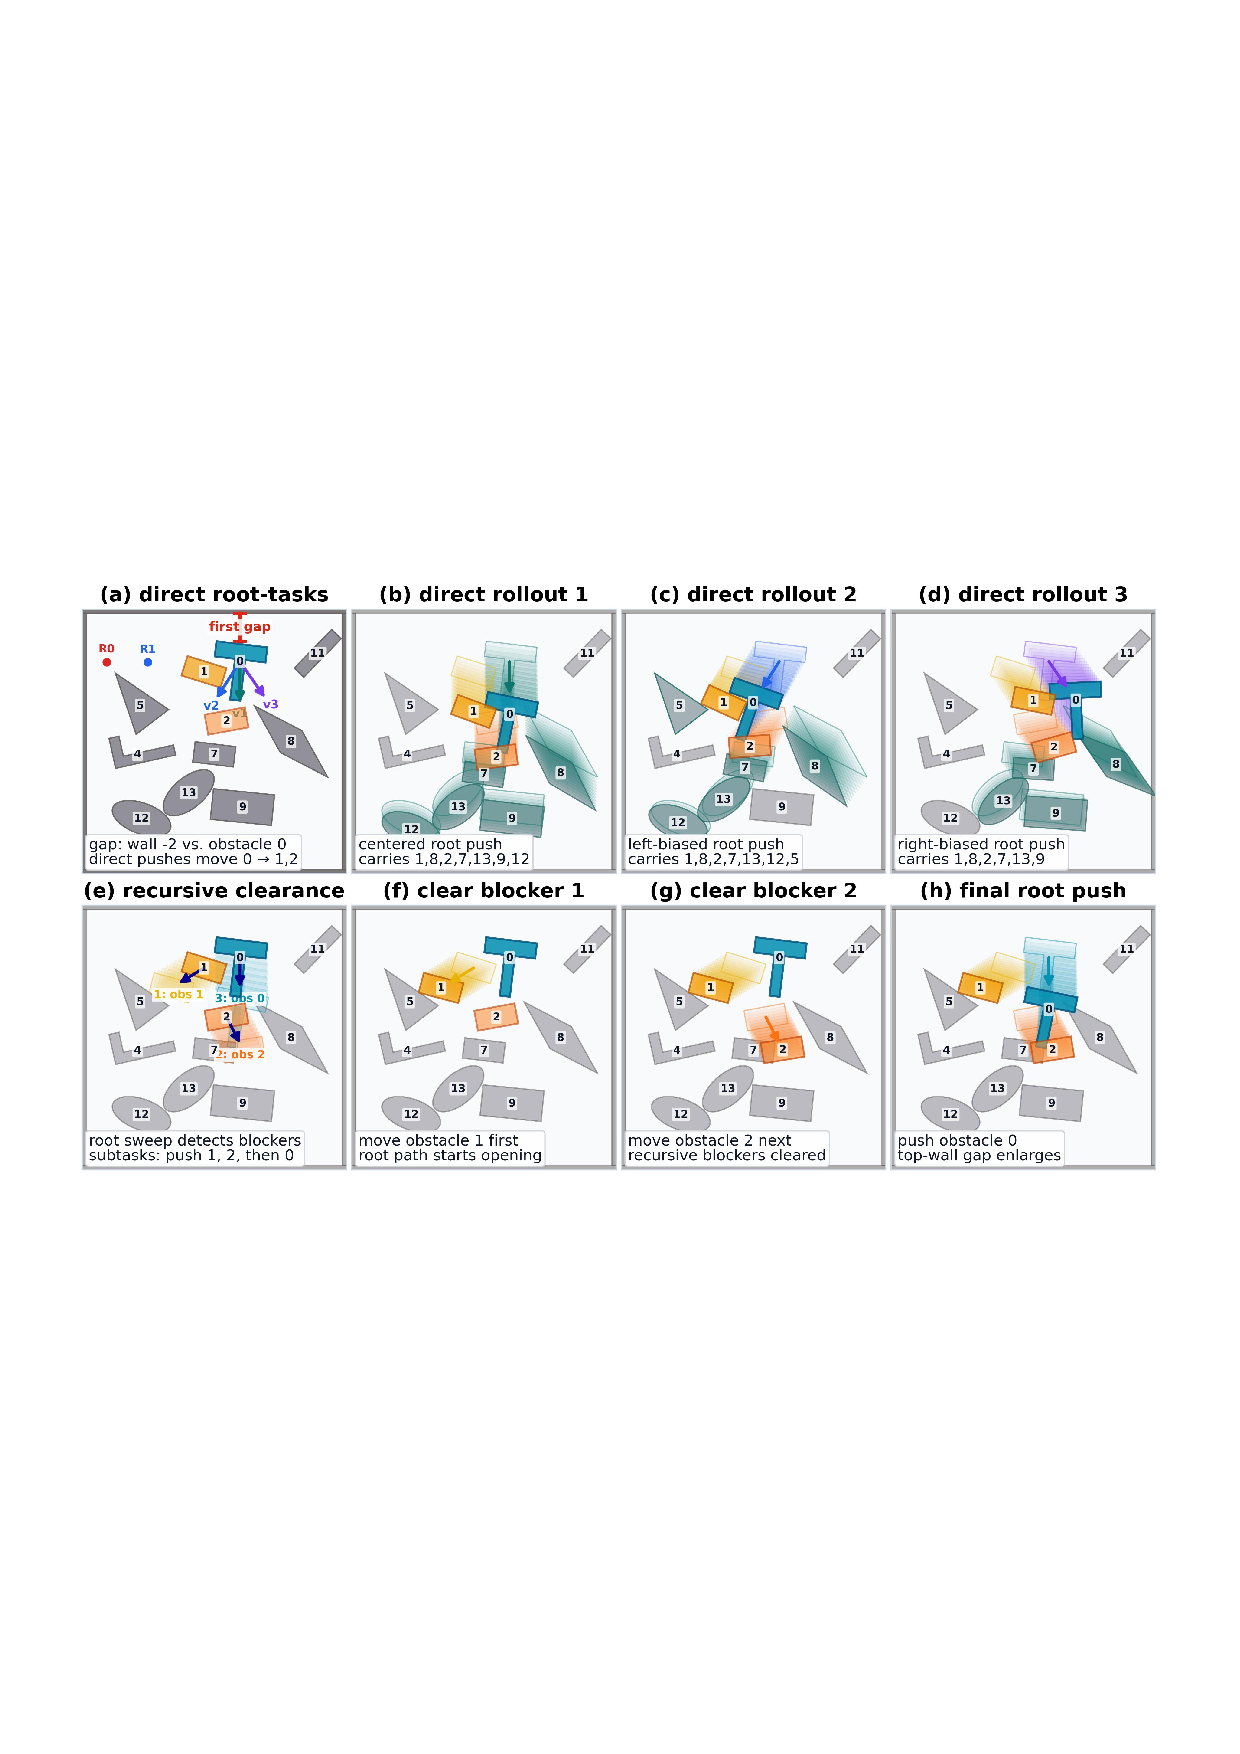
\includegraphics[width=0.85\linewidth]{figures/direct_recursive_push.pdf}
  \vspace{-0.1in}
  \caption{\change{
  \textbf{Direct} pushing moves a gap-side blocker along a gap-opening direction,
  whereas \textbf{recursive} pushing first clears movable blockers in the swept
  region and then returns to the root gap-opening task.}}
  \label{fig:direct_recursive_push}
  \vspace{-4mm}
\end{figure}

%------------------------------

\subsubsection{Long-term Cost w.r.t. Goal}
Furthermore, to prioritize gaps closer to the goal, a heuristic is added to the evaluation,
i.e.,
$h(g)=\eta\,\big\|\mathbf{o}(g)-\mathbf{x}_\texttt{V}^{\texttt{G}}\big\|$,
with the scaling constant~$\eta>0$.
Lastly, a short A$^\star$-style presearch is adopted to cross
each candidate gap, recompute the next frontier, and continue for a limited
width and depth. The \emph{cost-to-connect} is predicted by:
\begin{equation}\label{eq:pred_cost}
\widehat{\mathsf{Cost}}(g)\triangleq
\mathsf{C}\!\big(g \mid \mathcal{L},\mathbf{s}_{\mathcal{R}}\big)
+\!\!\!\sum_{g'\in\Pi^\star(g)}\!\!\!\big{\{}\mathsf{C}(g' \mid \cdot)+h(g')\big{\}},
\end{equation}
where~$\Pi^\star(g)$ is the sequence of subsequent gaps discovered after virtually crossing~$g$. Consequently, the final output of this module is the ranked list of candidate gaps, i.e.,
$\textsf{Rank}\big(\Gamma_\mathcal{L}\big)
\triangleq \textbf{argsort}_{g\in\Gamma_\mathcal{L}}\widehat{\mathsf{Cost}}(g)$,
in ascending predicted cost. This
ordered set is passed to the hybrid search module, such that only the
promising gaps are expanded first.



% %% ========================================
%==============================================
\subsection{Pushing Mode Generation and Evaluation}\label{subsec:push}
For a selected frontier gap~$g$, this subsection constructs candidate
pushing strategies
$\Xi_g\triangleq\{(\Omega_m,\mathbf{v},\boldsymbol{\xi})\}$,
where $\mathbf{v}=(v_x,v_y,\omega)\in\mathbb{R}^3$ is a short-horizon pushing
direction for~$\Omega_m$, and $\boldsymbol{\xi}=(\mathbf{c}_m,\mathbf{u})$
is its mode in~\eqref{eq:transition}.
\change{Wrench feasibility screens contact configurations that can realize
the required motion within actuation limits. The forces certify feasibility
rather than serving as hardware setpoints; candidate motion is then checked
by rollout or quick-pass reuse.}



%==============================================
\subsubsection{Direct and Recursive Pushing Tasks}
For \emph{direct push}, let~$\Omega_m$ denote one of the two movable obstacles adjacent to~$g$. For
each such obstacle, a small set of candidate body velocities
$\{\mathbf{v}_m^k\}_{k=1}^{K_m}$ is sampled with a bias toward enlarging the
gap~$g$, while a few angular components are included to account for local
geometry. If the swept region of a direct push intersects movable blockers,
\emph{recursive push} tasks are required instead: for each out-layer
blocker~$\Omega_m$, the nominal direction moves it away from both the swept
region and the reference gap sequence~$\Pi^\star(g)$. Recursion therefore
creates a bounded dependency chain which prioritizes the final
blocker~$\Omega_m$, as shown in Fig.~\ref{fig:direct_recursive_push}.






%==============================================
% \subsubsection{Pushing Mode Generation}
% For each sampled direction~$\mathbf{v}_m^k$ and obstacle~$\Omega_m$, the
% quality of a candidate mode is measured in the body frame. Let
% $\mathbf{v}_m^{k,\mathrm{B}} \in \mathbb{R}^3$ denote~$\mathbf{v}_m^k$
% expressed in the body frame of~$\Omega_m$. For a mode~$\boldsymbol{\xi}$,
% define the primary and multi-directional feasibility losses by:
% \begin{equation}\label{eq:mode-feasibility}
% \begin{aligned}
%   \mathrm{J}_{\texttt{F}}^m
%   (\boldsymbol{\xi},\mathbf{v}_m^{k,\mathrm{B}})
%   &\triangleq
%   \underset{\mathbf{q}_{m,\boldsymbol{\xi}} \in
%   \mathrm{Q}_{m,\boldsymbol{\xi}}}{\textbf{min}}
%   \left\|
%   \mathbf{q}_{m,\boldsymbol{\xi}} +
%   Q_\mu^m(\mathbf{v}_m^{k,\mathrm{B}})
%   \right\|_1,\\
%   \mathrm{J}_{\texttt{MF}}^m
%   (\boldsymbol{\xi},\mathbf{v}_m^{k,\mathrm{B}})
%   &\triangleq
%   \sum_{\mathbf{v}_d \in \mathcal{D}} w_d \cdot
%   \mathrm{J}_{\texttt{F}}^m(\boldsymbol{\xi},\mathbf{v}_d);
% \end{aligned}
% \end{equation}
% where~$\mathbf{q}_{m,\boldsymbol{\xi}} \in \mathbb{R}^3$ is the generalized
% body wrench induced by mode~$\boldsymbol{\xi}$;
% $\mathrm{Q}_{m,\boldsymbol{\xi}} \subseteq \mathbb{R}^3$ is the corresponding
% set of admissible body wrenches under the contact and friction constraints;
% $Q_\mu^m(\mathbf{v}_m^{k,\mathrm{B}}) \in \mathbb{R}^3$ denotes the
% quasi-static friction wrench of~$\Omega_m$ at direction~$\mathbf{v}_m^{k,\mathrm{B}}$;
% $\mathcal{D} \subset \mathbb{R}^3$ is a finite
% set of basis velocities containing the desired direction;
% and~$w_d > 0$ is the
% weight associated with~$\mathbf{v}_d \in \mathcal{D}$. Thus,
% small~$\mathrm{J}_{\texttt{F}}^m(\boldsymbol{\xi},\mathbf{v}_m^{k,\mathrm{B}})$ is
% necessary for force feasibility, while small
% $\mathrm{J}_{\texttt{MF}}^m$ indicates a robust mode.
% Accordingly, the associated mode
% $\boldsymbol{\xi}_m^k \triangleq (\mathbf{c}_m^k,\mathbf{u}_m^k)$ is generated
% by sparse optimization over the reachable part of~$\partial\Omega_m$. The
% reachable boundary is discretized into candidate contacts, and a sparse linear
% program (LP) is solved to minimize
% $\mathrm{J}_{\texttt{MF}}^m(\boldsymbol{\xi},\mathbf{v}_m^{k,\mathrm{B}})$
% under the local friction and wrench constraints.
% Detailed derivations are omitted here for brevity,
% and referred to~\cite{tang2024collaborative,tang2025pushingbots}.
% The resulting nonzero contacts provide~$\mathbf{c}_m^k$, and the corresponding forces
% yield~$\mathbf{u}_m^k$. Only the best few
% pairs~$(\mathbf{v}_m^k,\boldsymbol{\xi}_m^k)$ are retained and collected
% into~$\Xi_g$.

\subsubsection{Pushing Mode Generation}
At a search state~$\mathbf{s}$, a pushing mode is generated for each candidate
direction~$\mathbf{v}_m^k$ and obstacle~$\Omega_m$. In this subsubsection,
contact tuples, object velocities, forces, and wrenches are expressed in the
body frame of~$\Omega_m$. For a contact tuple~$\mathbf{c}$, its
multi-directional force feasibility is:
\begin{equation}\label{eq:mode-feasibility}
\mathrm{J}_{\texttt{MF}}^m(\mathbf{c},\mathbf{v}_m^k)
\triangleq
\sum_{\mathbf{v}_d\in\mathcal{D}_m^k} w_d
\underset{\mathbf{u}\in{U}_m(\mathbf{c})}{\textbf{min}}
\|
\mathbf{q}_m(\mathbf{c},\mathbf{u})
+\mathbf{q}_m^\mu(\mathbf{v}_d)
\| ,
\end{equation}
where~$\|\cdot\|$ is a weighted $\ell_1$ wrench norm, the finite set
$\mathcal{D}_m^k$ perturbs~$\mathbf{v}_m^k$, and
$\mathbf{q}_m^\mu(\mathbf{v}_d)$ is the quasi-static friction wrench; the inner
minimization is a small LP over the admissible forces ${U}_m(\mathbf{c})$.
A state- and direction-dependent contact set
$\mathcal{A}_m^k(\mathbf{s})\subset\partial\Omega_m$ is drawn from the
robot-reachable boundary of~$\Omega_m$ by velocity--force compatibility
filtering (Fig.~\ref{fig:mode_generation}), keeping a contact only if its
robots reach collision-free pre-contact poses. Starting from cached layouts or
random initializations, the tuple is refined by sequential greedy replacement:
at step~$\ell$, let $\mathbf{c}_{r,c}^{\ell}$ replace contact~$r$
with~$c$; select:
\begin{equation}
c^\star
=
\underset{c\in\mathcal{A}_m^k(\mathbf{s})}{\textbf{argmin}}\;
\mathrm{J}_{\texttt{MF}}^m
\bigl(\mathbf{c}_{r,c}^{\ell},\mathbf{v}_m^k\bigr),
\label{eq:greedy_mode_update}
\end{equation}
swept over contact slots until $\mathrm{J}_{\texttt{MF}}^m$ no longer
decreases or a bounded evaluation budget is reached.
The best tuple over initializations gives
$\mathbf{c}_m^{k,\star}$, from which $\mathbf{u}_m^k$ follows from the inner
minimization in~\eqref{eq:mode-feasibility}, yielding
$\boldsymbol{\xi}_m^k=(\mathbf{c}_m^{k,\star},\mathbf{u}_m^k)$; each mode is
cached as a warm start. \change{If the sequential replacement cannot assign a
contact to every robot, a bounded backtracking search over robot--contact
combinations (with a bounded budget) attempts the full-team assignment. If no feasible full-team mode is found
within this budget, for instance on small faces or under the pairwise
pusher-clearance constraint, one robot is temporarily left inactive and the
assignment is repeated with the remaining team. Reduced-team modes
carry a ranking penalty, so a feasible full-team mode is preferred, and the
inactive robot returns for the next task.} The best few admissible pairs are kept for gap~$g$ and
passed to simulation; $\mathbf{u}_m^k$ certifies wrench feasibility while
hardware tracks the contact geometry from pose/velocity commands.

% The best refined mode over all initializations is denoted by
% $\boldsymbol{\xi}_m^k=(\mathbf{c}_m^k,\mathbf{u}_m^k)$.
% It is admitted only if its rollout is validated in simulation.
% Accepted modes are stored in a persistent \textsc{mode-cache},
% indexed by discretized shape, mass, available robot force, and pushing direction,
% and reused as warm starts.
%------------------------------
\begin{figure}[t!]
  \centering
  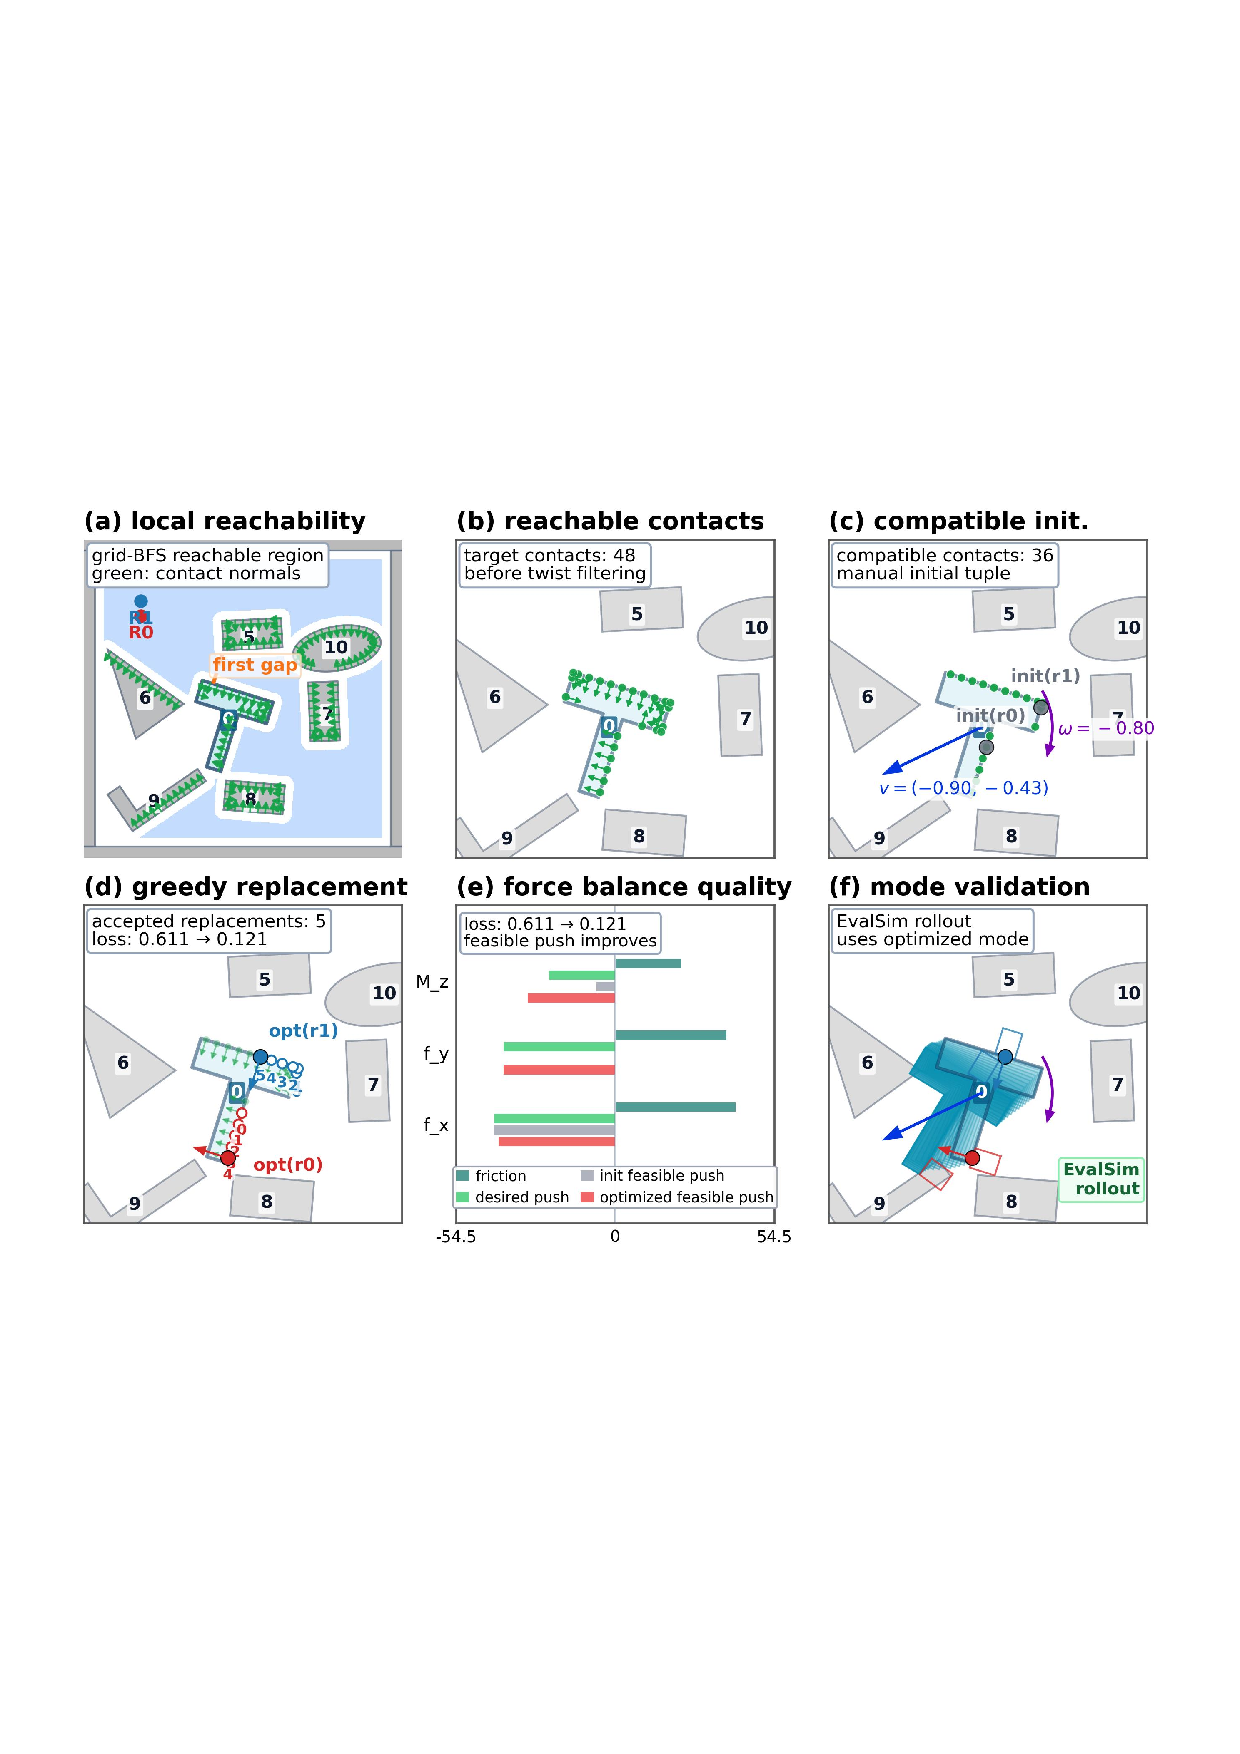
\includegraphics[width=0.85\linewidth]{figures/mode_generation.pdf}
  \vspace{-4mm}
  \caption{\change{Mode generation for a gap-opening task: (a) local reachability,
  (b) the reachable contact candidates after twist filtering, (c) a compatible
  initial contact tuple, (d) greedy replacement of individual contacts, (e) the
  force balance of the optimized push, and (f) rollout validation of the mode.}}
    \label{fig:mode_generation}
   \vspace{-4mm}
\end{figure}

%------------------------------
%==============================================
\subsubsection{Pushing Strategy Evaluation}

For a current state~$\mathbf{s}$ and candidate strategy
$(\Omega_m,\mathbf{v},\boldsymbol{\xi})\in\Xi_g$, a short-horizon rollout
evaluates the transition in~\eqref{eq:transition} under the selected mode.
As shown in Fig.~\ref{fig:mode_generation}, a strategy is accepted if the
robots reach the pre-contact poses, maintain stable contact and induce
obstacle motion above threshold. The simulation returns:
\begin{equation}
    (\mathbf{s}',\,\delta_{\texttt{T}},\,\delta_{\texttt{J}})
    \triangleq
    \mathsf{EvalSim}
    \big(
    \mathbf{s},(\Omega_m,\mathbf{v},\boldsymbol{\xi})
    \big),
    \label{eq:sim}
\end{equation}
where $\mathbf{s}'$ contains the resulting robot and object configurations,
$\delta_{\texttt{T}}>0$ is duration and $\delta_{\texttt{J}}$ control effort.
\change{Joint rollout captures contact-induced interactions among all bodies.
\minorchange{For quick-pass, a mode-table entry can store a validated body-frame state
sequence and cost increments. Under uniform, isotropic nominal dynamics,
translation invariance permits reuse for matching relative states, contacts,
twist, duration and physical properties (shape, mass, inertia, friction and
robot force limits), after reachability and robot--object swept-clearance
checks. Transforming the endpoint gives $\mathbf{s}'$ and cached increments
give $\delta_{\texttt{T}}$, $\delta_{\texttt{J}}$; uninvolved bodies remain
unchanged. Small parameter differences make reuse approximate.}}
%------------------------------
\begin{figure}[t!]
  \centering
  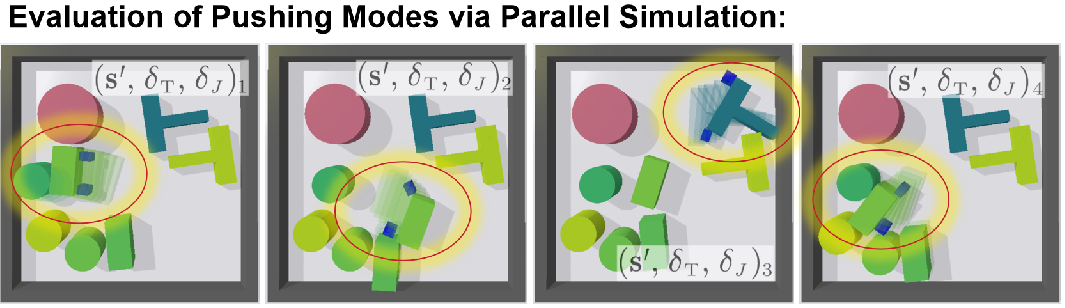
\includegraphics[width=0.95\linewidth]{figures/PIHS_bottom.pdf}
  \vspace{-2mm}
  \caption{\change{Sampled push tasks are evaluated via parallel simulation,
  producing updated states for search expansion.}}
    \label{fig:PIHS}
   \vspace{-4mm}
\end{figure}

%------------------------------

% %% ========================================
%==============================================
\subsection{Physics-Informed Hybrid Search}\label{subsec:simloop}

\change{The physics-informed hybrid search (PIHS) selects blocking gaps and
evaluates pushing strategies in parallel
(Fig.~\ref{fig:PIHS}, Alg.~\ref{alg:pihs}), \minorchange{using short-horizon simulation or
the nominal-model quick-pass reuse of Sec.~\ref{subsec:push}.}
Equation~\eqref{eq:problem} defines the evaluated clearance cost of a partial
schedule, used as the accumulated-cost term in the node priority
of~\eqref{eq:priority}.
Finite sampling gives no global optimality or completeness guarantee.}
\subsubsection{Tree and Initialization}
The search tree~$\mathcal{T}$ holds nodes
$\nu\triangleq(\mathbf{s},\pi)$, where~$\mathbf{s}$ is the system state of all
robots and movables in~\eqref{eq:transition} and~$\pi$ the partial pushing
strategy in~\eqref{eq:schedule}. Two global functions are maintained:
$\mathsf{Rank}(\nu)$ stores the ranked candidate
gaps~$\Gamma_{\mathcal{L}_\nu}$ of the frontier loop~$\mathcal{L}_\nu$ together
with their exploration costs by~\eqref{eq:pred_cost}, and~$\chi(\nu)$ returns
the cumulative execution cost from the root to~$\nu$. The root is
$\nu_0\triangleq(\mathbf{s}_0,\emptyset)$.
% At initialization,~$\chi(\nu_0)=0$, and
% $\mathsf{Rank}(\nu_0)$ is constructed by computing~$\Gamma_{\mathcal{L}_{\nu_0}}$
% for state~$\mathbf{s}_0$.

\subsubsection{Node Selection}
At each iteration, the node with minimum best-first priority is selected from
the queue. Priority balances realized cost and estimated remaining effort:
\begin{equation}\label{eq:priority}
  f(\nu)\triangleq \chi(\nu)+\underset{g\in \textsf{Rank}(\nu)}{\textbf{min}}
  \widehat{\mathsf{Cost}}(g),
\end{equation}
where~$\chi(\nu)$ is the cumulative execution cost so far, and the second term
is the minimum predicted remaining cost among the unexplored gaps of~$\nu$.
\change{The remaining-cost term is a heuristic and is not required to be admissible. The score prioritizes nodes by realized cost and promising future actions, but it does not provide an A* optimality guarantee.}



\begin{figure*}[t!]
  \centering
  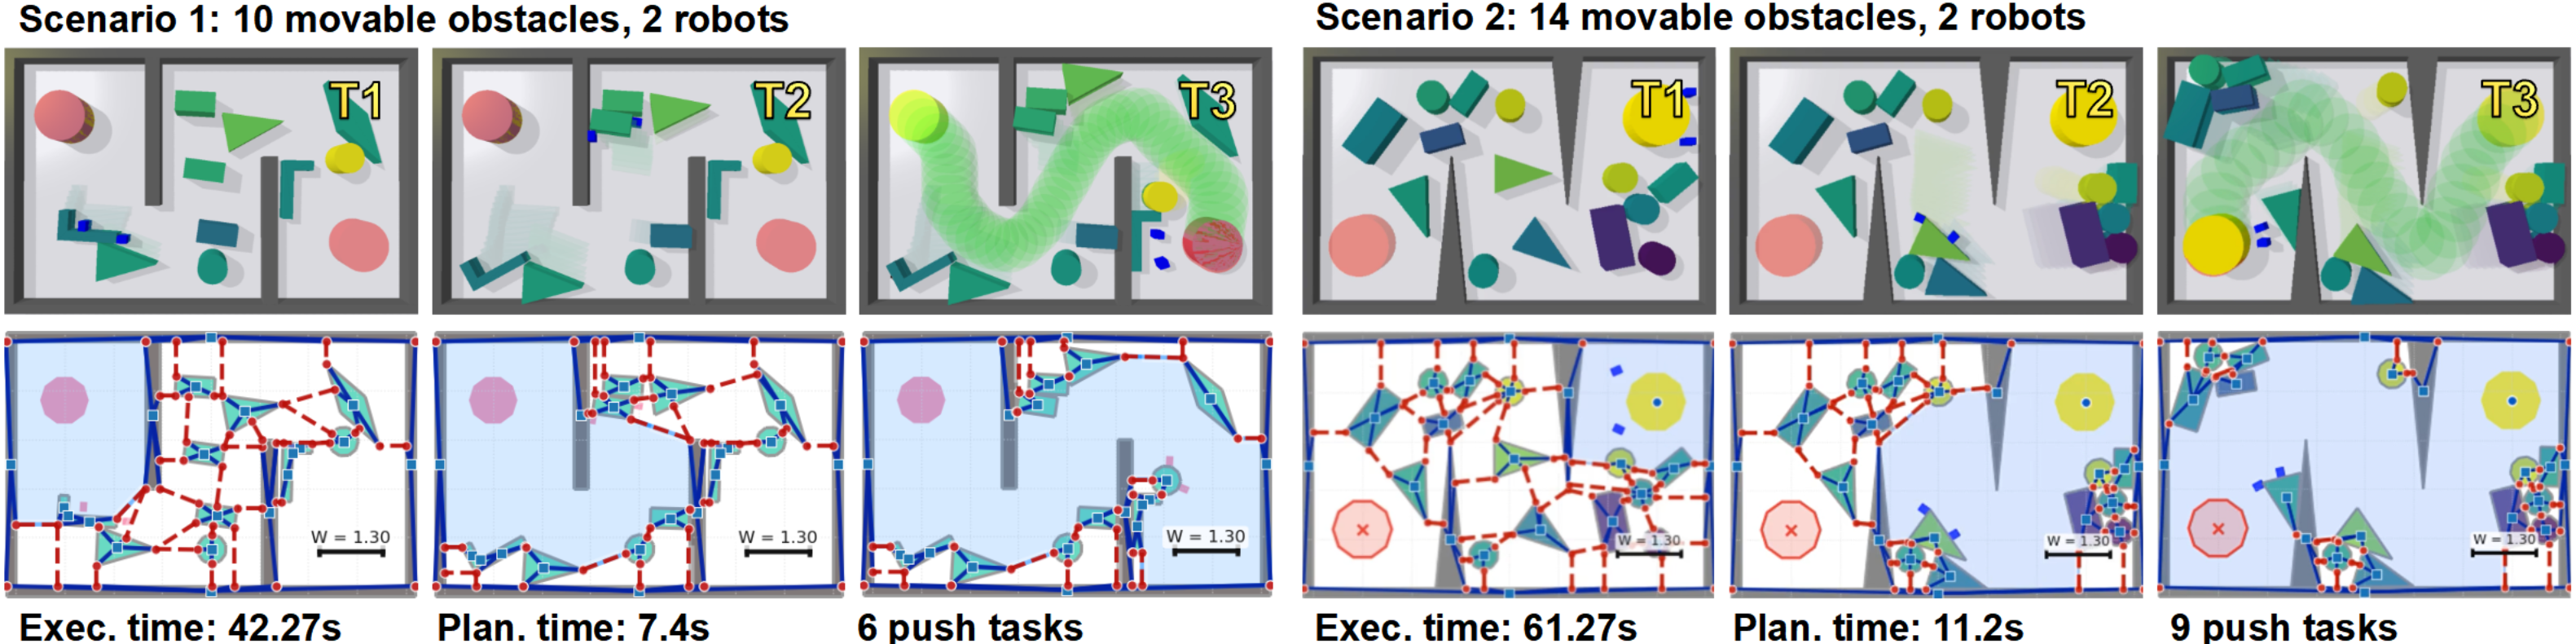
\includegraphics[width=0.95\linewidth]{figures/sim_fixed.png}
  \vspace{-2mm}
  \caption{\change{Execution and planning alignment in Scenario 1 (\textbf{Left})
    and  Scenario 2 (\textbf{Right}).
\textbf{Top:} simulated snapshots during path clearing.
\textbf{Bottom:} corresponding WCCG overlays with the start face in blue.
The executed pushes progressively expand the reachable $W$--clearance region until the goal is connected.}}
\vspace{-6mm}
\label{fig:main_result}
\end{figure*}
% ========================================

% ========================================
\subsubsection{Node Expansion with Parallel Simulation}
Let the selected node be~$\nu \triangleq (\mathbf{s},\pi)$. For each ranked gap
$g \in \mathsf{Rank}(\nu)$,
its predicted gap sequence~$\Pi^\star(g)$ in~\eqref{eq:pred_cost}
is first derived. Then, the mode optimization by~\eqref{eq:mode-feasibility}
provides a candidate strategy set
$\Xi_g \triangleq \{(\Omega_m,\mathbf{v},\boldsymbol{\xi})\}$,
including both the direct push of the adjacent movable obstacles,
and recursive push of out-layer obstacles.
Thus, expansion is prioritized first by the gap ordering in
$\mathsf{Rank}(\nu)$, and then by the candidate ordering within~$\Xi_g$.
\minorchange{Each candidate is evaluated by~\eqref{eq:sim}, using quick-pass reuse
or a rollout as described in Sec.~\ref{subsec:push}.}
A successful evaluation yields
$(\mathbf{s}',\delta_{\texttt{T}},\delta_{\texttt{J}})$, from which a child
node~$\nu' \triangleq (\mathbf{s}',\pi')$ is created with
$\pi' \triangleq \pi \cup \{\tau\}$, appending
$\tau \triangleq (\Omega_m,\mathbf{v},\boldsymbol{\xi})$ to the current partial
schedule~$\pi$.
The cumulative cost is updated by:
$\chi(\nu') \triangleq \chi(\nu) + \widehat{\mathsf{C}}(\nu,\tau)$,
where~$\widehat{\mathsf{C}}(\nu,\tau)\triangleq
\delta_{\texttt{T}} + \alpha\,\delta_{\texttt{J}}$
\change{is the evaluated incremental cost.}
Thereby, one expansion can yield several validated successors.


{
\SetAlFnt{\small}
\SetAlgoSkip{0pt}
%==============================================
\begin{algorithm}[t!]
\caption{Physics-Informed Hybrid Search}\label{alg:pihs}
\SetAlgoLined
\KwIn{$\mathbf{s}_0$,~$\alpha$,~$\mathsf{EvalSim}(\cdot)$,~$W$--criterion by~\eqref{eq:wccg_criterion}}
\KwOut{Clearing schedule $\pi^\star$, or failure}
$\nu_0\gets(\mathbf{s}_0,\emptyset),\;\chi(\nu_0)=0$\;
Init~$\mathcal{Q}$ by~\eqref{eq:priority}\;
\While{$\mathcal{Q}\ne\emptyset$ and budget remains}{
 $\nu=(\mathbf{s},\pi)\gets\mathcal{Q}.\texttt{pop\_min}()$ by~\eqref{eq:priority}\;
 \If{$\mathbf{s}$ admits~$\mathcal{P}^W_{\texttt{V}}$ by~\eqref{eq:wccg_criterion}}{
  \Return $\pi$\;
 }
  \ForEach{$g\in\mathsf{Rank}(\nu)$}{
    Compute~$\Pi^\star(g)$, generate~$\Xi_g$\;
    \ForEach{$(\Omega_m,\mathbf{v},\boldsymbol{\xi})\in\Xi_g$}{
      $\tau=(\Omega_m,\mathbf{v},\boldsymbol{\xi})$ \tcp{Direct or recur.}
      $(\mathbf{s}',\delta_\texttt{T},\delta_\texttt{J})\gets\mathsf{EvalSim}(\nu,\tau)$
      by~\eqref{eq:sim}\;
    \If{success}{
     $\pi'\gets\pi\cup\{\tau\}$\;
     $\nu'\gets(\mathbf{s}',\pi')$\;
     $\chi(\nu')\gets\chi(\nu)+\delta_\texttt{T}+\alpha\,\delta_\texttt{J}$\;
     Add $\nu'$ to $\mathcal{Q}$\;
      }
    }
  }
}
\Return failure;
\end{algorithm}
%==============================================
}
%==============================

\subsubsection{Termination}
Termination occurs when a node~$\nu$ reaches a state~$\mathbf{s}$ for which a
$W$--clear path~$\mathcal{P}^W_\texttt{V}$ exists from
$\mathbf{x}_\texttt{V}^{\texttt{S}}$ to~$\mathbf{x}_\texttt{V}^{\texttt{G}}$
by~\eqref{eq:wccg_criterion}. \change{Thus, $\pi$ encodes both the gaps to clear
and the strategies that realize them, satisfying nominal clearance and
evaluated pushing transitions. This does not imply global minimization
of~$\mathcal{J}_{\mathrm{clr}}$. The objective covers clearing only;
vehicle traversal follows afterwards.}

\begin{remark}\label{remark:simloop}
\change{Gap-lookahead reduces unproductive branches, \textsc{mode-cache}
warm-starts optimization, \minorchange{and quick-pass reuses validated transitions
to avoid redundant rollouts.}}
\hfill$\blacksquare$
\end{remark}

% %%========================================
%==============================
\subsection{Overall Analyses}\label{subsec:overall}

\subsubsection{Execution and Online Adaptation}\label{subsec:execute}
The hybrid search returns a pushing schedule
$\pi = \{\tau_1,\cdots,\tau_K\}$, with
$\tau_k \triangleq (\Omega_k,\mathbf{v}_k,\boldsymbol{\xi}_k)$.
The schedule is executed in a receding-horizon manner: for each $\tau_k$ the
robots reach the mode~$\boldsymbol{\xi}_k$ and follow the pushing
direction~$\mathbf{v}_k$ from the current state, as in~\eqref{eq:sim}.
\change{On the hardware the optimized contact forces certify feasibility rather
than being commanded: a mode is retained only if its object wrench lies within
the robots' actuation limits, and over each control interval $\mathsf{EvalSim}$ predicts a short forward
object-motion reference (the expected displacement and rotation of the object),
which the velocity-level controller tracks with motion-capture feedback, and each
executed push returns an observed state that re-enters the planner.} During transitions,
robots are reassigned by preserving the circular order of contact points along
the obstacle boundary~\cite{tang2026pushingbots}, reducing path crossings under
sufficient clearance. After each push the state is updated from observation,
the WCCG is rebuilt from the current configuration, and execution continues
until a $W$-clear path
$\mathcal{P}^W_\texttt{V}$ connects~$\mathbf{x}_\texttt{V}^{\texttt{S}}$ and
$\mathbf{x}_\texttt{V}^{\texttt{G}}$.
Replanning is triggered by observed execution discrepancies -- failed contact
establishment, stalled pushing, or invalidated WCCG connectivity -- in which
case Alg.~\ref{alg:pihs} is called from the current state to derive the
updated schedule.

%----------------------------------------------
\subsubsection{Computational Complexity}\label{subsubsec:complexity}

Given~$M$ movable obstacles, the computational cost of one node
expansion in Alg.~\ref{alg:pihs} is dominated by candidate generation and
physics validation. The WCCG update and gap ranking incur
$\mathcal{O}(M\log M+|\mathcal{V}|+|\mathcal{E}_c|+|\mathcal{E}_b|)$ and
$\mathcal{O}(|\Gamma_{\mathcal{L}_\nu}|
\log|\Gamma_{\mathcal{L}_\nu}|)$ costs, respectively.
\change{The dominant simulation cost
$\mathcal{O}\big(\sum_{g\in\mathsf{Rank}(\nu)}|\Xi_g|\,\big(C_{\mathrm{LP}}+\rho_\nu T_{\mathrm{sim}}/n_{\texttt{w}}\big)\big)$
grows with the number of validated candidates and is reduced by the
$n_{\texttt{w}}$ parallel workers, so scalability is set by validated
candidates rather than by the enumeration of contact assignments.} \change{Robot-team size mainly affects mode
generation: the greedy stage evaluates at most $N|\mathcal{A}|$ single-contact
substitutions instead of the exhaustive $|\mathcal{A}|^N$ assignment, and when it
fails, a bounded-backtracking search over robots and candidates expands at most
$B{=}2000$ partial assignments, a fixed budget independent of the team size; the
subset fallback repeats this search for at most one excluded robot. The number
of LP feasibility checks per task is therefore at most
$(N|\mathcal{A}|{+}2B)$, each over the $2N$ admissible contact forces, rather
than growing as $|\mathcal{A}|^N$.}
%% %----------------------------------------------
%% \subsubsection{Generalization}\label{subsec:general}
%% The framework admits several extensions:
%% (I) \textit{Heterogeneous teams.} Per-robot gain tuning and robot-specific mode
%% priors enable cooperation among diverse robots;
%% (II) \textit{Concurrent pushing.} Multi-object mode generation and conflict-aware
%% transition planning allow multiple obstacles to be pushed simultaneously;
%% (III) \textit{Dynamic environments.} Periodic $W$--connectivity checks and
%% on-demand replanning handle disturbances such as object drift or unmodeled
%% contacts during execution.

% %%========================================

%%========================================
% ============================================================
\section{Experiments}
\label{sec:experiments}
We evaluate PIHS in simulation and hardware (see accompanying video).
The algorithms are implemented in \texttt{Python3} and \texttt{PyBullet}~\cite{coumans2019}
on a machine with an Intel i9-14900KF and an RTX 4080.
\subsection{Numerical Simulations}
\label{subsec:sim}
% ========================================
\begin{table}[t]

\centering

\caption{\change{WCCG connectivity validation and mean runtime.}}

\label{tab:wccg-validation}

\vspace{-2.0mm}

\footnotesize

\setlength{\tabcolsep}{3.8pt}
\setlength{\belowrulesep}{0.30ex}
\renewcommand{\arraystretch}{0.86}

\change{
\begin{tabular}{
 @{}
 l
 cc
 @{\hspace{8pt}}
 ccc
 @{}
}

\toprule

&
\multicolumn{2}{c}{Validation}
&
\multicolumn{3}{c}{Runtime (ms)}
\\[-0.6ex]

\cmidrule(lr){2-3}
\cmidrule(lr){4-6}

Type
& CC $=$ FR
& FP/FN$^\dagger$
& CC
& FR
& WCCG
\\

\midrule

Convex
& 100/100
& 0/0
& 1.23
& 282.9
& \textbf{0.86}
\\

Non-convex
& 98/100
& 0/0
& 1.51
& 204.1
& \textbf{1.30}
\\

Mixed
& 98/100
& 0/0
& 1.33
& 242.4
& \textbf{1.05}
\\

\midrule

Total
& 296/300
& \textbf{0/0}
& 1.36
& 243.1
& \textbf{1.07}
\\

\bottomrule

\end{tabular}
}

\vspace{0.5mm}

{\scriptsize
\change{
$^\dagger$WCCG errors relative to the continuous configuration-space reference (CC).
All runtimes use the same 300-scene harness with the compiled WCCG backend.
}
}

\vspace{-5.5mm}

\end{table}

\subsubsection{Setup and Configuration}\label{subsec:sim-setup}

The simulation runs at a step size of $\Delta t=1/240$\,s with a control period
of $1/40$\,s; robots are disk or box pushers consistent with the $W$-clearance
definition, and movable obstacles have masses $[5,15]$\,kg in Scenarios~1--2, $[20,30]$\,kg in the generalization studies. A trial
succeeds when the external vehicle reaches its goal through a $W$-clear path. The
nominal scenario is an $8\times5$\,m workspace with bottleneck-forming bar
obstacles, where two robots clear $10$--$15$ movable obstacles under
minimum-separation constraints. Unless stated otherwise, comparisons and
ablations use Scenario~1 ($10$ movable obstacles, $40$ trials), and Scenario~2
($14$ obstacles) provides an additional cluttered case
(Fig.~\ref{fig:main_result}). \change{All methods share the robot footprints,
obstacle configurations, collision and reachability checks, and execution
simulator, with the same $800$\,s planning cap, $20{,}000$-step ($500$\,s) execution cap and $8$ workers. Unless stated otherwise, times average over successful trials, failures counting only in the success rate; the scalability curves instead cap failures.}



% ========================================
\begin{table}[t]
 \centering
 \begin{threeparttable}
 \caption{Performance comparison and ablations on Scenario~1 over $40$ randomized trials.\tnote{a}}
 \label{tab:main_ablation}
 \setlength{\tabcolsep}{2.7pt}
 \renewcommand{\arraystretch}{0.92}
 \begin{tabular}{lccccc}
 \toprule
 Method / Variant & Succ.(\%) & PT (s) & ET (s) & \#Sims & \#Pushes \\
 \midrule
 DFS-WCCG & 25.0 & $>$100.0 & 51.2 & $>$500 & 8.0 \\
 SL-Push (offline) & 62.5 & 0.06 & 44.1 & 0.0 & 7.3 \\
 SL-Push (sim) & 75.0 & 18.2 & 64.6 & 20.0 & 10.2 \\
 Rec-NAMO & 37.5 & 13.3 & 42.4 & 0.0 & 7.8 \\
 \textbf{PushAround (ours)}
 & \textbf{97.5} & \textbf{10.3} & \textbf{28.6}
 & \textbf{121.5} & \textbf{6.0} \\
 \midrule
 w/o gap-lookahead & 82.5 & 16.9 & 35.2 & 178.3 & 7.2 \\
 w/o mode-cache & 92.5 & 17.1 & 33.4 & 164.6 & 6.5 \\
 w/o quick-pass & 90.0 & 23.6 & 41.9 & 208.2 & 6.1 \\
 w/o reinsertion & 85.0 & 12.8 & 31.1 & 151.7 & 7.8 \\
 \bottomrule
 \end{tabular}
 \begin{tablenotes}\scriptsize
 \item[a] Times are averaged over successful trials; failures count in the
 success rate only. For DFS-WCCG, $PT$ and
 \#Sims are not comparable and are given as lower bounds ($>$).
 \end{tablenotes}
 \end{threeparttable}
 \vspace{-4.0mm}
\end{table}

% ========================================
% ========================================
\begin{figure}[t!]
 \centering
 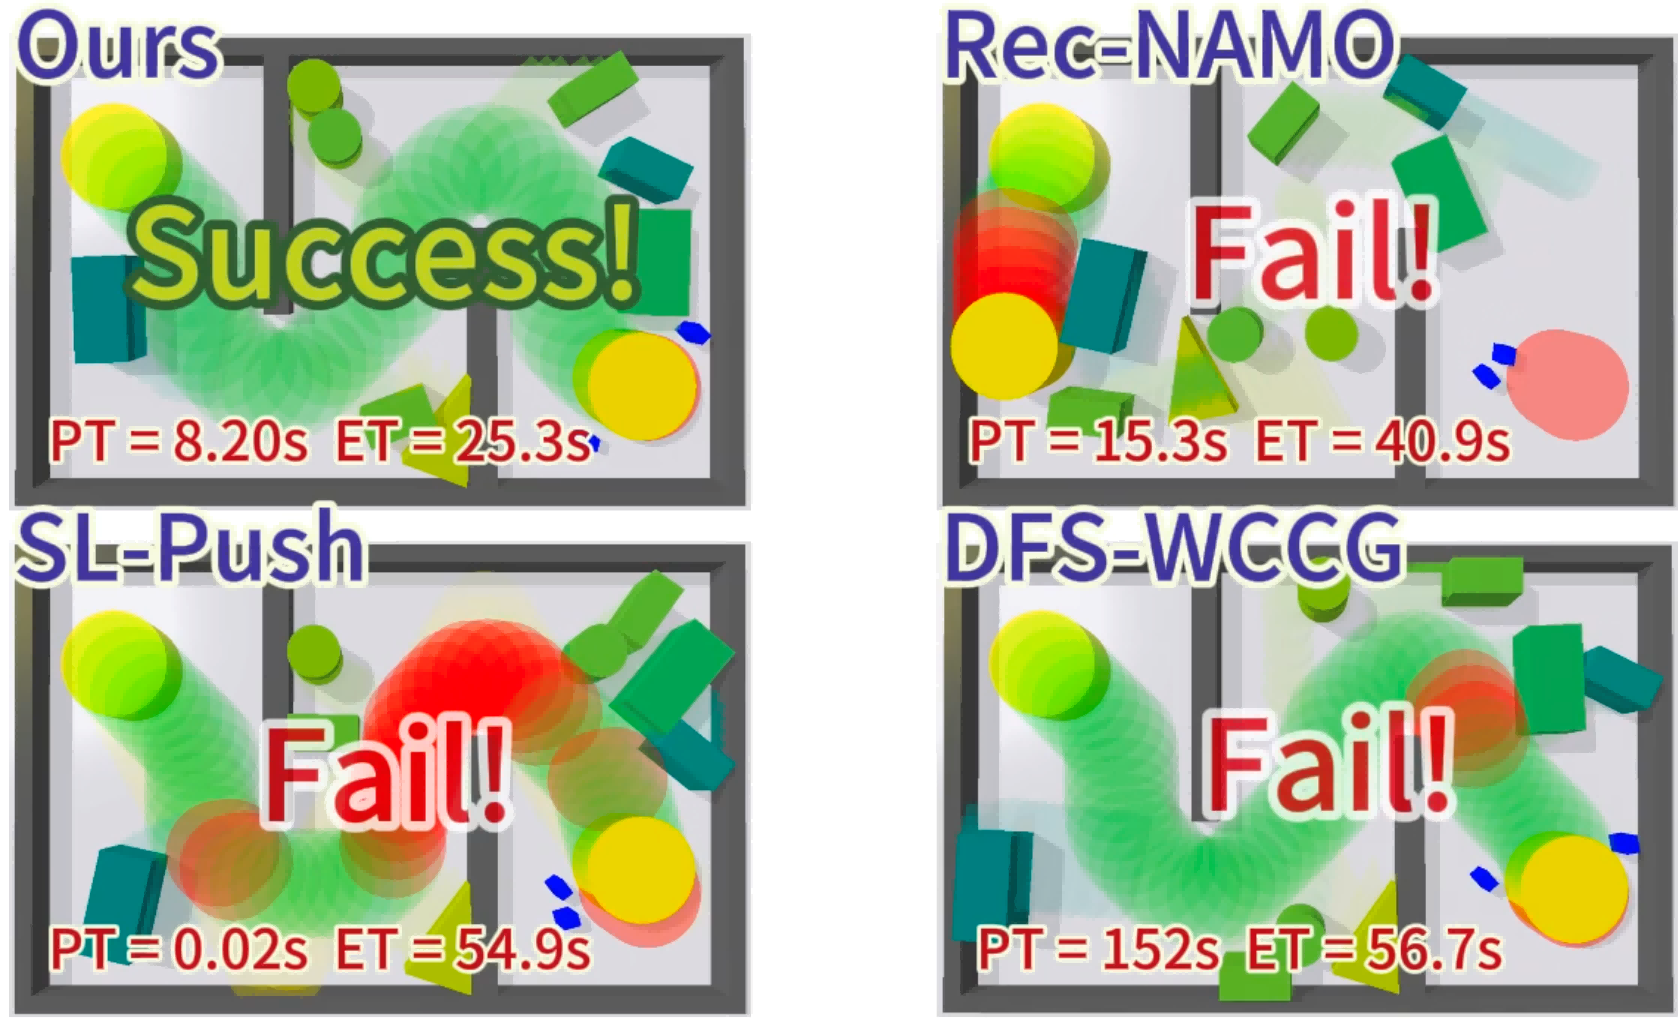
\includegraphics[width=0.7\columnwidth]{figures/compare.png}
 \vspace{-3.0mm}
 \caption{Failure cases by baselines Rec-NAMO, SL-Push and DFS-WCCG.}
 \label{fig:baseline}
 \vspace{-6.0mm}
\end{figure}

% ========================================
%==============================
\subsubsection{Results}
\change{
Across the $40$ Scenario~1 trials, PushAround achieves a $97.5\%$ success rate,
with mean planning and execution times of $10.3$\,s and $28.6$\,s, respectively,
and $6.0$ pushes per successful trial, as shown in Table~\ref{tab:main_ablation}.
Fig.~\ref{fig:main_result} shows representative runs in both scenarios.
In Scenario~1 with $10$ movable obstacles and two robots, PushAround generates
a $6$-push plan in $7.4$\,s and completes execution in $42.3$\,s. In
Scenario~2 with $14$ obstacles, it generates a $9$-push plan in $11.2$\,s,
with $61.3$\,s of execution.
Planning effort is dominated by simulation-based validation: a successful
trial uses $121.5$ simulations on average for $6.0$ executed pushes. The
ablations indicate that mode caching, quick-pass, gap lookahead, and reinsertion
mainly affect this validation load rather than plan length. Execution takes
longer because each selected push is physically carried out and observed,
whereas inter-push repositioning is handled by geometric reachability checks.
}

\change{
\subsubsection{WCCG Connectivity Validation}
\label{subsec:wccg-validation}

WCCG is compared against two references on $300$ random scenes (convex,
non-convex and mixed; Table~\ref{tab:wccg-validation}). The continuous reference (CC) resolves collisions geometrically after inflating boundaries by~$W/2$, with no grid discretization~\cite{lozano1983spatial}; the fine-raster reference (FR) discretizes the workspace on a $0.01$\,m occupancy grid. CC and FR disagree in $4$ of $300$ cases, all near narrow contacts and rasterization-related, whereas WCCG matches CC on all $300$ scenes without false positives or negatives. A query costs $1.07$\,ms ($0.67$\,ms query, $0.40$\,ms construction)
against $1.36$\,ms (CC) and $243$\,ms (FR). It also supplies the gap graph for PIHS. Rebuilt after every simulated or executed push, it is negligible next to the physics rollouts.
}




\subsubsection{Comparisons}\label{subsec:comparisons}
Four baseline variants run on Scenario~1 over $40$ randomized trials under the same $W$-clearance criterion, distribution and simulator:
\textbf{DFS-WCCG} (WCCG-guided search with fixed pushes), \textbf{SL-Push}
(offline and simulation-validated variants), and \textbf{Rec-NAMO} (recursive
NAMO)~\cite{stilman2007manipulation,yao2024local,saxena2023planning,ren2025search}.
Table~\ref{tab:main_ablation} shows that PushAround reaches the highest success
rate, $97.5\%$, at the lowest combined planning-and-execution time among
successful trials ($38.9$\,s).
DFS-WCCG exhibits rapid branching growth, offline SL-Push produces displacements that fail in execution, and Rec-NAMO often fails to connect the $W$-clear corridor in clutter (Fig.~\ref{fig:baseline}).


%==============================
\begin{table}[t]

\caption{\change{Scalability and robustness.}}
\label{tab:generalization}
\vspace{-2.0mm}
\centering
\footnotesize

\renewcommand{\arraystretch}{0.95}
\setlength{\tabcolsep}{3.5pt}

\change{
\begin{tabular}{
 @{}
 l
 c
 c
 r@{\;}c@{\;}l
 @{\hspace{10pt}}
 r@{\;}c@{\;}l
 @{}
}
\hline

Case
& Trials
& Succ.(\%)
& \multicolumn{3}{c@{\hspace{10pt}}}{$PT$ (s)}
& \multicolumn{3}{c}{$ET$ (s)}
\\

\hline

\multicolumn{9}{l}{
 \emph{Obstacle density} (PushAround, $N=2$, nominal)
}
\\

$M=15$
& 10 & 100
& 2.5 & $\pm$ & 0.9
& 37.1 & $\pm$ & 21.0
\\

$M=30$
& 10 & 100
& 11.7 & $\pm$ & 3.7
& 100.9 & $\pm$ & 34.7
\\

$M=45$
& 10 & 100
& 53.4 & $\pm$ & 24.5
& 272.7 & $\pm$ & 97.4
\\

\hline

\multicolumn{9}{l}{
 \emph{Robot-team size} ($M=30$, nominal; 10 trials per cell)
}
\\

PushAround, $N=3$
& 10 & 100
& 30.0 & $\pm$ & 12.7
& 97.3 & $\pm$ & 42.1
\\

PushAround, $N=4$
& 10 & 100
& 29.2 & $\pm$ & 8.9
& 110.1 & $\pm$ & 33.1
\\

SL-Push (sim), $N=3$
& 10 & 80
& 30.0 & $\pm$ & 46.3
& 193.3 & $\pm$ & 111.3
\\

SL-Push (sim), $N=4$
& 10 & 80
& 23.4 & $\pm$ & 18.2
& 171.7 & $\pm$ & 61.2
\\

DFS-WCCG, $N=3$
& 10 & 100
& 142.6 & $\pm$ & 183.1
& 178.1 & $\pm$ & 72.1
\\

DFS-WCCG, $N=4$
& 10 & 90
& 101.9 & $\pm$ & 103.9
& 175.9 & $\pm$ & 113.6
\\

\hline

\multicolumn{9}{l}{
 \emph{Physics mismatch} ($M=30$, $N=2$)
}
\\

Nominal
& 10 & 100
& 16.8 & $\pm$ & 3.4
& 104.7 & $\pm$ & 37.4
\\

Mass $\times 0.6$--$1.4$
& 40 & 100
& 16.8 & $\pm$ & 5.4
& 105.9 & $\pm$ & 44.6
\\

Lateral fric. $\times 0.6$--$1.4$
& 40 & 97.5
& 16.5 & $\pm$ & 5.7
& 114.0 & $\pm$ & 48.5
\\

Spin fric. $\times 0.6$--$1.4$
& 40 & 97.5
& 15.2 & $\pm$ & 3.6
& 100.1 & $\pm$ & 35.7
\\

Force limit $\times 0.6$--$1.4$
& 40 & 95.0
& 18.9 & $\pm$ & 10.9
& 115.9 & $\pm$ & 58.5
\\

All perturbed
& 160 & 97.5
& 16.9 & $\pm$ & 7.0
& 108.9 & $\pm$ & 47.4
\\

\hline

\end{tabular}
}

\vspace{0.5mm}

\begin{flushleft}
\footnotesize
\change{
Each perturbed row scales one parameter; the others stay nominal. Times and budget
are as in Table~\ref{tab:main_ablation}.
}
\end{flushleft}

\vspace{-6.0mm}

\end{table}

%==============================

%==============================
\subsubsection{Ablation Studies}
Four internal ablations are conducted: \textbf{w/o gap-lookahead} (gaps ranked
without downstream costs), \textbf{w/o mode-cache} (no warm start from validated
modes), \textbf{w/o quick-pass} (all candidates evaluated by rollout), and
\textbf{w/o reinsertion} (failed nodes not reconsidered).
Table~\ref{tab:main_ablation} shows that gap-lookahead and reinsertion mainly
improve robustness (success drops by more than $10\%$ when either is removed),
whereas quick-pass also lowers success to $90.0\%$ and mode-cache mainly changes
the simulation count.


\change{

\subsubsection{Scalability and Robustness Analysis}
\label{subsec:generalization}

Generalization studies use an $8\times8$\,m workspace
(Table~\ref{tab:generalization}, Figs.~\ref{fig:scalability_scenes}--\ref{fig:density_scaling}).
\minorchange{Density runs query a precomputed mode table (preparation excluded from $PT$);
mismatch and team-size runs optimize modes greedily. At $M{=}30$, $N{=}2$,
nominal $PT$ is $11.7$, $16.8$ and $23.9$\,s, respectively; the team-size
study uses a different scene realization of the same seeds.}
\textbf{(I) Obstacle density:} with two robots, $10$ trials per density,
PushAround keeps $100\%$ success at all tested densities ($M{=}15$ to $45$), planning in $2.5$--$53.4$\,s; at $M{=}45$ none of the evaluated baselines solves any trial
and the no-recursion ablation solves $7/10$.
\textbf{(II) Robot-team size:} at $M{=}30$, PushAround solves all ten trials at
$N{=}2$, $3$, and $4$ using the same mode-generation
procedure with a full-team-first fallback that may leave one robot temporarily inactive.
Across the clutter sweep, branching stays near six while expansions rise
from $3.5$ to $24.5$. A solved trial needs a median of $10$ expansions and
$48$ visited snapshots and about $60$ simulations at $165$\,ms each,
against $22$\,ms per generated mode. Across $N{=}2$--$4$, search effort remains similar
($10$ expansions, $60$--$63$ simulations), while aggregate mode-generation
time rises from $15.8$ to $46.4$\,s.
\textbf{(III) Physics mismatch:} the planner keeps the nominal model and only
the execution simulator is perturbed, one parameter at a time.
PushAround solves $156/160$ perturbed trials ($97.5\%$); under $\pm40\%$
perturbations SL-Push (sim) solves $13/40$ and DFS-WCCG $23/40$.
Averaging successful-trial $PT$ over conditions with successes gives $31.5$
and $229.1$\,s, versus $18.4$\,s for PushAround.
\minorchange{These paired, single-parameter trials reuse ten base seeds (five for
baselines), whose nominal success is $3/5$ versus $10/10$ for PushAround.
Comparisons reflect end-to-end performance rather than normalized
degradation; joint parameter errors are untested.}

}



% ========================================
\begin{figure}[t!]
 \centering
 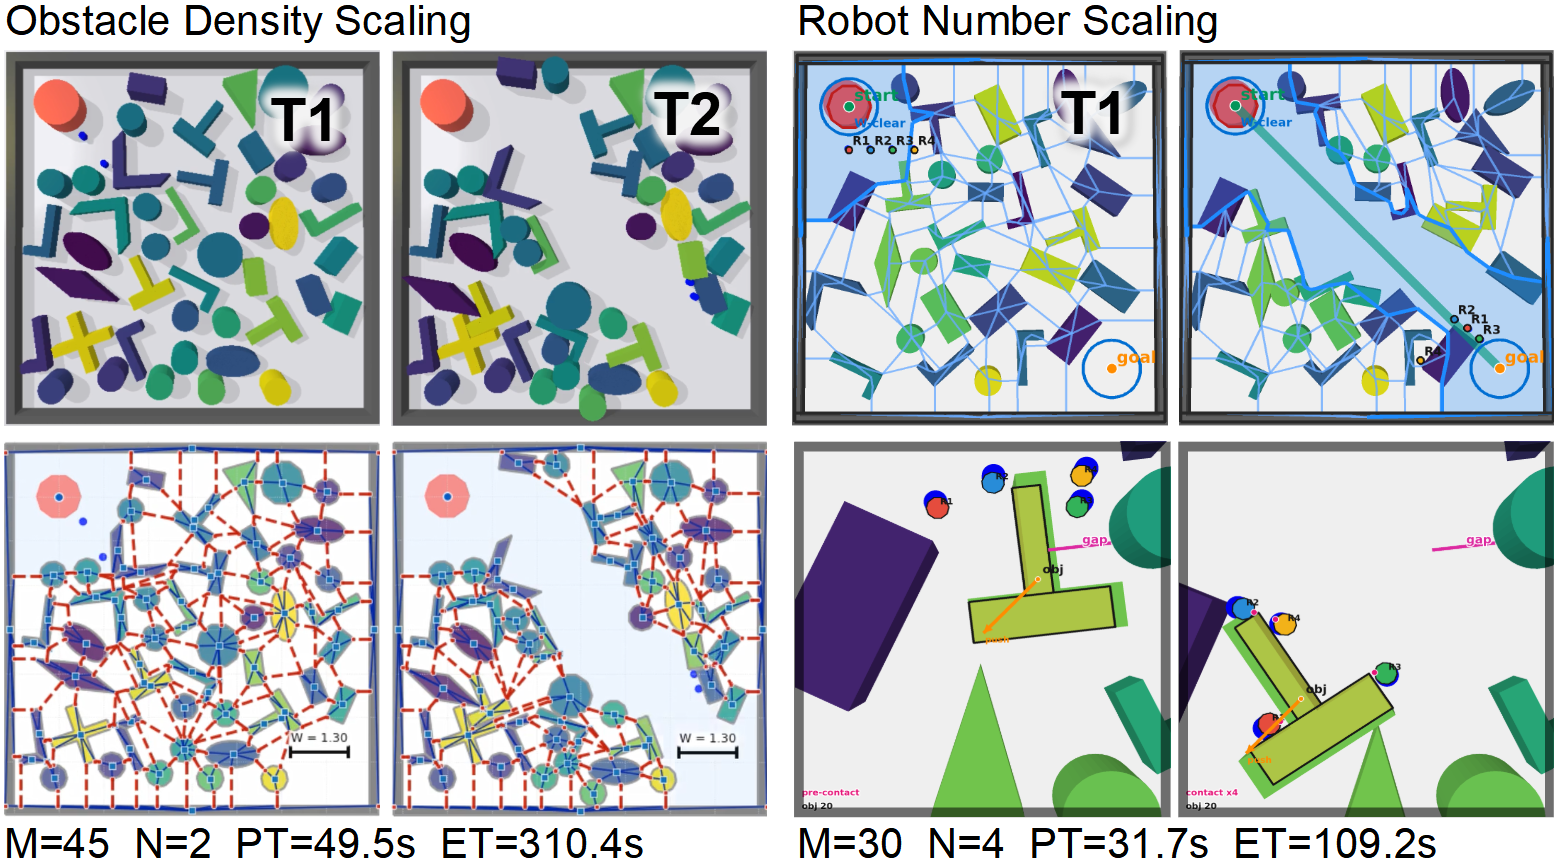
\includegraphics[width=0.9\columnwidth]{figures/obs_rob_scale.png}
 \vspace{-2mm}
 \caption{\change{
 Scalability of the clearing process. \textbf{Left:} density scaling ($M{=}45$, two robots): snapshots during clearing (\textbf{top}) and WCCG overlays with the start face in blue (\textbf{bottom}). \textbf{Right:} team scaling ($M{=}30$, four robots): initial and final states (\textbf{top}) and one push before contact and during execution (\textbf{bottom}).}}
 \label{fig:scalability_scenes}
 \vspace{-3mm}
\end{figure}

% ========================================
% ========================================
\begin{figure}[t!]
 \centering
 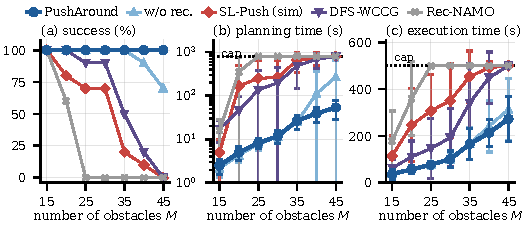
\includegraphics[width=0.95\columnwidth]{figures/density_comparison.pdf}
 \vspace{-2.0mm}
 \caption{\change{
 Obstacle-density scaling ($8\times 8$\,m, $10$ seeds per density). Times are
 budget-capped (planning $800$\,s, execution $20{,}000$ steps $=500$\,s; dotted).}}
 \label{fig:density_scaling}
 \vspace{-4.0mm}
\end{figure}

% ========================================
% ========================================
% ========================================
\begin{figure*}[!t]
 \centering
 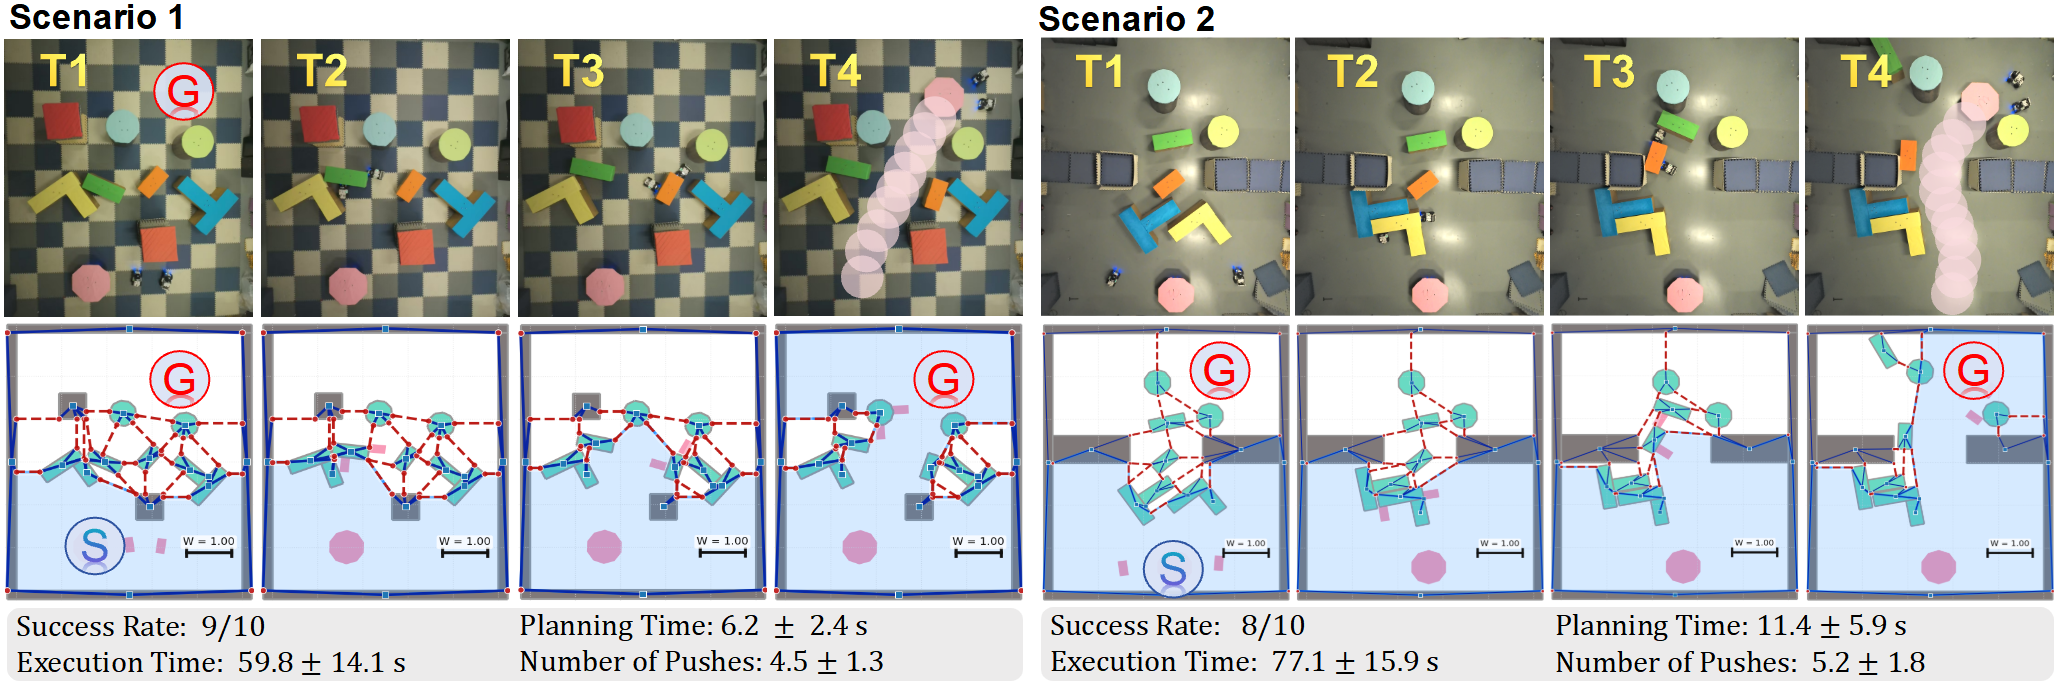
\includegraphics[width=0.95\linewidth]{figures/hardware.png}
 \vspace{-2.0mm}
 \caption{\change{Real-world pushing experiments with execution--planning alignment (over~$20$ runs, $2$ scenarios).
 \textbf{Top:} two robots pushing obstacles in a \(5{\times}6\,\mathrm{m}\)
 workspace. \textbf{Bottom:} WCCG overlays with the start face in blue.}}
 \vspace{-5.0mm}
 \label{fig:hardware}
\end{figure*}

\subsection{Hardware Experiments}\label{subsec:hardware}

\subsubsection{System Description}\label{subsec:exp-description}
Experiments use a $5\times6$\,m workspace of interlocking $0.6\times0.6$\,m foam mats (Fig.~\ref{fig:hardware}), $2$ UGVs and $6$ cardboard boxes; robots and movables carry motion-capture markers streamed to \texttt{PyBullet} in real time.
\change{The UGVs are velocity-controlled, and the optimized contact forces are used only for feasibility evaluation, not for motor control.
\minorchange{Motion-capture poses are compared with $\mathsf{EvalSim}$ predictions:
position or orientation errors above $0.3$\,m or $\pi/4$ trigger replanning,
as do the failures in Sec.~\ref{subsec:execute}.}}

\subsubsection{Results}\label{subsec:exp-results}
Two representative real-world runs are shown in Fig.~\ref{fig:hardware}.
In hardware Scenario~1, PIHS considers five candidate gaps and plans a four-task schedule in $6.5$\,s ($12$ node expansions, $49$ visited snapshots, search depth $6$); the robots then execute it, first rotating the yellow L-shaped object to open a gap near an
immovable obstacle and then separating the green and orange objects until a $W$--clear path is established at $t=52\,$s.
In hardware Scenario~2, PushAround succeeds in $8/10$ trials with an average of $5.2$
pushes and $11.4$\,s of planning; the first direct push on the blue L-shaped
object also moves the adjacent T-shaped block and opens the first gap.
\change{This neighboring-object motion is not a separately encoded action but
an emergent outcome of the coupled rigid-body rollout in $\mathsf{EvalSim}$,
whose snapshot updates the WCCG and execution continues.}
\change{\minorchange{Execution takes $77.1\pm15.9$\,s (mean $\pm$ standard deviation);}
online replanning compensates for deviations due to force limits,
drifting and wheel slippage.}

%%========================================
\section{Conclusion} \label{sec:conclusion}
\change{This work presents PushAround, a multi-robot framework that jointly plans
obstacle selection, contact points and pushing forces through a hybrid search,
and demonstrates hardware feasibility with state-feedback replanning. Future work
targets obstacle-state estimation without external sensing, uncertain masses and
limited robot visibility.}

%%========================================


%========================================
\bibliographystyle{IEEEtran}
\bibliography{contents/references}

\end{document}
